\documentclass[11pt,a4paper]{article}
\usepackage[margin=1in]{geometry}
\usepackage{lmodern}
\usepackage[protrusion=true,expansion=true]{microtype}
\usepackage{titling}
\usepackage{enumitem}
\usepackage{longtable}
\usepackage{booktabs}
\usepackage{graphicx}
\usepackage{tabularx}
\usepackage{caption}
\usepackage{pgfgantt}
\usepackage{tocloft}
\usepackage{float}
\usepackage{amsmath}
\usepackage{amssymb}
\usepackage{hyperref}
\usepackage{fancyhdr}
\usepackage{pgfplots}
\pgfplotsset{compat=1.18}
\usepackage{subcaption}
\graphicspath{{figures/}}

% Configure Table of Contents spacing
\setlength{\cftbeforesecskip}{8pt}
\setlength{\cftbeforesubsecskip}{4pt}

% Configure hyperref
\hypersetup{
    colorlinks=true,
    linkcolor=black,
    citecolor=black,
    urlcolor=black,
    pdfborder={0 0 0},
    pdftitle={Smart Healthcare Robot},
    pdfauthor={Almoulla Talal Almaawali, Abdulmunim Khamis Albusaidi}
}

% Configure page headers and footers (Academic Thesis Style)
\pagestyle{fancy}
\fancyhf{} % Clear all headers and footers
\fancyhead[L]{\small\textit{\leftmark}} % Left side: Section name
\fancyhead[R]{\small\textit{Smart Healthcare Robot}} % Right side: Document title
\fancyfoot[C]{\thepage} % Page number centered in footer
\renewcommand{\headrulewidth}{0.4pt}
\renewcommand{\footrulewidth}{0pt}
\renewcommand{\sectionmark}[1]{\markboth{#1}{}} % Properly set section marks

% Different style for chapter intro pages (no header, only page number)
\fancypagestyle{plain}{
    \fancyhf{}
    \fancyfoot[C]{\thepage}
    \renewcommand{\headrulewidth}{0pt}
}

\begin{document}

% ============================================================
% TITLE PAGE
% ============================================================
\begin{titlepage}
\centering
\vspace*{0.5cm}

% University Logo

\includegraphics[width=0.75\textwidth]{squ-logo-new.png}\\[0.5cm]

% University Header
{\Large\textbf{SULTAN QABOOS UNIVERSITY}}\\[0.4cm]
{\large College of Engineering}\\[0.3cm]
{\large Department of Electrical and Computer Engineering}\\[0.2cm]

\vspace{2cm}

% Project Title
{\Huge\textbf{Smart Healthcare Robot}}\\[0.8cm]
{\LARGE Bringing Care Closer to Patients in Oman}

\vspace{1.5cm}

% Authors
{\large\textbf{Almoulla Talal Almaawali \& Abdulmunim Khamis Albusaidi}}\\[0.3cm]
{\normalsize 135591 \& 133225}

\vspace{1cm}

% Supervisor
{\large\textbf{Supervisor:}}\\[0.3cm]
{\large Ahmed Chehib Ammari}

\vspace{1.5cm}

% Degree Statement
{\normalsize A Final Year Project Report submitted to the Department of}\\
{\normalsize Electrical and Computer Engineering, Sultan Qaboos University}\\
{\normalsize in partial fulfilment of the requirements for the Degree of}

\vspace{0.5cm}

{\large\textbf{BACHELOR OF ENGINEERING}}\\
{\normalsize in}\\
{\large\textbf{ELECTRICAL \& COMPUTER ENGINEERING}}

\vfill

% Date
{\large Academic Year 2025--2026}\\[0.4cm]
{\normalsize December 2025}

\end{titlepage}

% ============================================================
% STUDENTS DECLARATION STATEMENT
% ============================================================
\newpage
\thispagestyle{empty}
\section*{Students Declaration Statement}
\addcontentsline{toc}{section}{Students Declaration Statement}

We certify that Mr. Almoulla Talal Almaawali (Student ID: 135591) and Mr. Abdulmunim Khamis Albusaidi (Student ID: 133225) that this project is our own work, based on our personal study and that we have acknowledged all material and sources used in its preparation, whether they be books, articles, reports, lecture notes, and any other kind of document, electronic or personal communication.

We also certify that this report does not include any violation of anyone's copyrights or otherwise plagiarised the work of other persons.

\vspace{2cm}

\noindent
\begin{tabular}{@{}p{0.4\textwidth}p{0.5\textwidth}@{}}
. . . . . . . . . . . . . . . . . . . . . & . . . . . . . . . . . . . . . . . . . . . \\
Date: December 13, 2025 & Students's Names \\
& Almoulla Talal Almaawali \\
& Abdulmunim Khamis Albusaidi
\end{tabular}

% ============================================================
% DECLARATION OF AI USE
% ============================================================
\newpage
\thispagestyle{empty}
\section*{Declaration of Generative AI and AI-Assisted Technologies}
\addcontentsline{toc}{section}{Declaration of AI Use}

During the preparation of this work, the students Almoulla Talal Almaawali (Student ID: 135591) and Abdulmunim Khamis Albusaidi (Student ID: 133225) used generative AI tools including ChatGPT, Claude, and Google Gemini in order to assist with literature review synthesis, technical writing refinement, code documentation. After using these tools, the students reviewed and edited the content as needed and take full responsibility for the accuracy, integrity, and originality of the content presented in this Final Year Project report.

% ============================================================
% ABSTRACT
% ============================================================
\newpage
\thispagestyle{empty}
\section*{Abstract}
\addcontentsline{toc}{section}{Abstract}

This project develops a smart healthcare robot for Omani hospitals to assist medical staff with routine tasks. The robot uses ROS~2 for autonomous navigation, LiDAR-based SLAM for mapping, and Google Gemini 3 flash for natural language interaction. It can deliver items, guide patients, and provide information through a tablet interface.

Three platform alternatives were evaluated using AHP decision matrices. A hybrid architecture was selected, combining a commercial robot base with custom AI layers. The system includes seven subsystems: Mobility, Navigation, Perception, Intelligence, Task Management, Interface, and Power Management. The design addresses healthcare workforce challenges while maintaining patient safety and ease of use.

\vspace{0.5cm}
\noindent\textbf{Keywords:} Healthcare Robotics, Autonomous Mobile Robots, ROS 2, LiDAR SLAM, Human--Robot Interaction, Large Language Models

% ============================================================
% GRAPHICAL ABSTRACT
% ============================================================
\newpage
\thispagestyle{empty}
\section*{Graphical Abstract}
\addcontentsline{toc}{section}{Graphical Abstract}
\begin{figure}[H]
    \centering
    \includegraphics[width=0.95\textwidth]{visual-abstract-1765608906756.png}
    \caption*{Graphical abstract of the proposed autonomous mobile robot for hospital logistics and its evidence-based benefits in clinical environments.}
\end{figure}

% ============================================================
% ACKNOWLEDGEMENT
% ============================================================
\newpage
\thispagestyle{empty}
\section*{Acknowledgement}
\addcontentsline{toc}{section}{Acknowledgement}

We acknowledge our supervisor, Dr. Ahmed Chehib Ammari, for his guidance throughout this project.

We thank the Department of Electrical and Computer Engineering at Sultan Qaboos University for providing the necessary facilities and resources.

% ============================================================
% ACRONYMS
% ============================================================
\newpage
\thispagestyle{empty}
\section*{Acronyms}
\addcontentsline{toc}{section}{Acronyms}

\begin{tabular}{@{}ll@{}}
\toprule
\textbf{Acronym} & \textbf{Description} \\
\midrule
AHP & Analytic Hierarchy Process \\
AI & Artificial Intelligence \\
AMR & Autonomous Mobile Robot \\
API & Application Programming Interface \\
BMS & Battery Management System \\
EHR & Electronic Health Record \\
GDPR & General Data Protection Regulation \\
HIPAA & Health Insurance Portability and Accountability Act \\
HIS & Hospital Information System \\
HRI & Human--Robot Interaction \\
IMU & Inertial Measurement Unit \\
LiDAR & Light Detection and Ranging \\
LLM & Large Language Model \\
ROS & Robot Operating System \\
SLAM & Simultaneous Localization and Mapping \\
ToF & Time of Flight \\
UWB & Ultra-Wideband \\
WBS & Work Breakdown Structure \\
\bottomrule
\end{tabular}

% ============================================================
% TABLE OF CONTENTS
% ============================================================
\newpage
\tableofcontents
\newpage

% ============================================================
% LIST OF FIGURES
% ============================================================
\listoffigures
\newpage

% ============================================================
% LIST OF TABLES
% ============================================================
\listoftables
\newpage

% ============================================================
% MAIN CONTENT
% ============================================================
\setcounter{page}{1}

% Chapter intro page macro (book-like divider)
\newcommand{\chapterintro}[3]{%
\clearpage
\thispagestyle{empty}%
\vspace*{2cm}%
\begin{center}
    {\fontsize{72}{72}\selectfont \textbf{#1}}\\[0.6cm]
    {\LARGE\bfseries #2}\\[0.6cm]
    \rule{0.75\textwidth}{0.6pt}\\[0.6cm]
    \parbox{0.75\textwidth}{\large #3}
\end{center}
\vfill
\clearpage
}

% Chapter 1: Introduction
\chapterintro{1}{Introduction}{This chapter establishes the project context, problem statement, motivation, objectives, methodology overview, and the project management plan that frames execution for the rest of the report.}
\section{Introduction}
\label{sec:introduction}

\subsection{Project Context}
Modern healthcare systems worldwide face an urgent mandate to deliver safe, accessible, and high-quality care to growing populations. However, the post-pandemic era has highlighted critical vulnerabilities: the risk of infection during routine contact, the strain on medical staff, and the logistical burden of managing hospital wards \cite{frontiers2024}.

In modern hospitals, a significant portion of nursing time is spent on non-clinical logistics. This manual workload not only reduces patient care time but also increases staff exposure to hazardous waste and infectious diseases. This project introduces an autonomous robotic solution designed to automate these routine tasks, ensuring safety and efficiency in healthcare facilities.


\subsection{Problem Statement}
Oman's healthcare system strives to reach all citizens, with government local health services reaching 100\% of urban families and 90\% of rural families \cite{alsheikhly2006}, yet geographic distances and resource constraints create barriers to timely and accessible care for the remaining underserved populations. Existing telepresence solutions often rely on manual control and lack the ability to engage patients in even basic diagnostic dialogue. This results in increased workloads for healthcare providers and a less personalized, less effective experience for patients, particularly those in rural areas or with mobility limitations.


\subsection{Motivation}
Every day in Oman, patients need medical attention that could be provided remotely if the right tools existed. Children in hospitals need comfort when parents cannot be present. Elderly patients need medication reminders and someone to check on their well-being. Rural communities need access to specialist consultations without long journeys.

The global demand for remote healthcare solutions is growing rapidly, with the telepresence robot market expected to experience significant growth. More importantly, Oman's Vision 2040 calls for healthcare innovation that serves all citizens equally, regardless of location \cite{alhinai2024}. Recent studies have shown that telemedicine adoption in Oman's primary healthcare settings demonstrates both promise and areas for improvement \cite{alsalmani2023}, while infrastructure requirements for effective telemedicine networks continue to be refined \cite{alshishtawy2013}. The aim of the project is to design and implement a smart telepresence robot with autonomous indoor navigation and on-device basic triage dialogue for ward corridors and bedside spaces in hospitals in Oman.

\subsection{Objectives}

\begin{itemize}[leftmargin=*]
    \item To develop a robust autonomous navigation system capable of dynamic obstacle avoidance and Simultaneous Localization and Mapping (SLAM) in crowded hospital corridors.

    \item To engineer a secure telepresence interface that enables real-time, low-latency audio/visual consultations for remote doctors.

    \item To integrate an AI-driven interaction layer (using Large Language Models) to provide basic triage, visitor guidance, and patient reassurance.

    \item To validate the system in a pilot scenario, demonstrating successful autonomous delivery (Nurse Station $\rightarrow$ Bed) and remote consultation cycles.
\end{itemize}


\subsection{Methodology}
The project begins with a systematic requirements analysis informed by a literature review and a healthcare facility needs assessment. Following this, we evaluate and select optimal design alternatives for both the hardware platform and software architecture using the Analytic Hierarchy Process (AHP) methodology. The development follows an iterative prototyping cycle, beginning with establishing reliable remote teleoperation, advancing to implementing and refining the autonomous navigation system, and culminating in integrating the conversational AI dialogue capabilities. Finally, the system undergoes real-world validation in simulated and pilot clinical settings to measure performance metrics such as navigation reliability, telepresence quality of service, and overall user experience for both patients and clinical staff.


\subsection{Project Management Plan}
The project timeline spans two academic semesters, from September 2025 to May 2026. The first semester focuses on research, requirements analysis, and conceptual design, while the second semester is dedicated to implementation, testing, and final evaluation.

\begin{figure}[H]
    \centering
    \resizebox{\textwidth}{!}{%
    \begin{ganttchart}[
        vgrid={*1{draw=black!40, line width=1.2pt}},
        hgrid={*1{draw=black!10, dotted}},
        x unit=1.5cm,
        y unit chart=0.8cm,
        time slot format=isodate-yearmonth,
        time slot unit=month,
        title/.style={draw=none, fill=none},
        title label font=\bfseries\small,
        title label node/.append style={below=7pt},
        include title in canvas=false,
        bar label font=\small\color{black!80},
        bar/.append style={fill=blue!40, draw=none, rounded corners=2pt},
        bar height=0.5,
        bar top shift=0.25,
        group right shift=0,
        group top shift=0.7,
        group height=.3,
        group peaks width={0.2},
        milestone/.append style={fill=red!70, draw=none, rounded corners=2pt},
        milestone label font=\small\itshape
    ]{2025-09}{2026-05}
    \gantttitlecalendar{year, month=shortname} \\
    
    % Semester 1
    \ganttgroup{Semester 1: Planning \& Design}{2025-09}{2025-12} \\
    \ganttbar{Project Initiation}{2025-09}{2025-09} \\
    \ganttbar{Literature Survey}{2025-10}{2025-10} \\
    \ganttbar{Requirements Specs}{2025-11}{2025-11} \\
    \ganttbar{Conceptual Design}{2025-12}{2025-12} \\
    \ganttmilestone{Interim Report}{2025-12} \\

    % Semester 2
    \ganttgroup{Semester 2: Implementation}{2026-02}{2026-05} \\
    \ganttbar{Hardware Assembly}{2026-02}{2026-02} \\
    \ganttbar{Software Dev (Nav, UI, LLM)}{2026-02}{2026-03} \\
    \ganttbar{System Integration}{2026-04}{2026-04} \\
    \ganttbar{Testing \& Validation}{2026-04}{2026-05} \\
    \ganttmilestone{Final Report}{2026-05}
    \end{ganttchart}
    }
    \caption{Project Gantt Chart (Sep 2025 - May 2026)}
    \label{fig:gantt_chart}
\end{figure}

\subsubsection{Work Breakdown Structure (WBS)}
The detailed tasks and responsibilities are outlined in Table \ref{tab:wbs}.

\begin{table}[H]
\centering
\caption{Work Breakdown Structure (WBS)}
\label{tab:wbs}
\renewcommand{\arraystretch}{1.3}
\begin{tabularx}{\textwidth}{@{}l X l l@{}}
\toprule
\textbf{Phase} & \textbf{Task Description} & \textbf{Deliverables} & \textbf{Assigned To} \\
\midrule

\textbf{Phase 1} & Project Initiation & Problem Statement & Both \\
\textit{(Sep 2025)} & Methodology Definition & Methodology Section & Both \\
\addlinespace[0.5em]

\textbf{Phase 2} & Literature Review & Literature Survey & Both \\
\textit{(Oct 2025)} & Research Gap Analysis & Gap Identification & Both \\
\addlinespace[0.5em]

\textbf{Phase 3} & Requirements Analysis & Requirements Doc & Both \\
\textit{(Nov 2025)} & Constraints Analysis & Eng. Constraints & Both \\
\addlinespace[0.5em]

\textbf{Phase 4} & Conceptual Design & Design Alternatives & Both \\
\textit{(Dec 2025)} & Functional Decomposition & System Architecture & Both \\
\addlinespace[0.5em]

\textbf{Phase 5} & Implementation: Hardware & Assembled Robot & Almoulla \\
\textit{(Feb-Mar)} & Implementation: Navigation & Autonomous Nav & Almoulla \\
 & Implementation: UI & Clinician/Patient GUI & Abdulmunim \\
 & Implementation: LLM & Voice Interaction & Almoulla \\
\addlinespace[0.5em]

\textbf{Phase 6} & Testing \& Finalization & Integrated System & Both \\
\textit{(Apr-May)} & Final Report Writing & Final Thesis & Both \\

\bottomrule
\end{tabularx}
\end{table}


% Chapter 2: Literature Review
\chapterintro{2}{Literature Review}{This chapter surveys consumer, industrial, and healthcare robotics; documents benefits and challenges of AMRs in hospitals; analyzes core technologies (navigation, RF localization, SLAM, LLMs); and motivates the platform choices and project needs.}
\section{Literature Review}
\label{sec:literature-review}
\subsection{Motivation and State of the Field}

The integration of robotics and artificial intelligence into healthcare is advancing rapidly, driven by challenges such as aging populations, rising healthcare costs, and medical staff shortages. Researchers have developed various robotic solutions, including telepresence robots for remote consultations, autonomous robots for logistics, and socially assistive robots (SARs) for patient engagement. While each type has proven useful, they often function in isolation, addressing only part of patients' and clinicians' overall needs. The goal is to show that although the components for such a system already exist, combining them into a single, user-friendly, and autonomous platform remains an underexplored area with high potential, especially for improving healthcare accessibility in regions like Oman.

Telepresence robots, often described as a mobile screen, are widely used for remote medical consultations. Systems such as InTouch Health RP-VITA and the VGo robot have been used successfully in "telestroke" care, allowing neurologists to assess patients remotely, reduce diagnosis time, and improve outcomes \cite{garingo2016}. These systems support remote rounds, specialist consultations, and family visits, cutting travel costs and reducing infection risks. However, studies also note several drawbacks. A review by Kristoffersson et al. found that telepresence robots, though functional, often feel impersonal and difficult to control \cite{kristoffersson2013}. Clinicians report high cognitive load when navigating cluttered hospital spaces. Patients, especially the elderly and children, also find these robots less engaging than in-person visits due to limited physical embodiment and lack of expressive cues \cite{sabanovic2013}. This "presence gap" limits their effectiveness beyond basic video conferencing, reducing their ability to offer comfort and reassurance during care.

This literature review builds a comprehensive case for an integrated, autonomous healthcare robotics platform. It begins by examining success stories from consumer and industrial robotics, demonstrating that autonomous navigation technology has reached maturity and widespread adoption. The review then analyzes healthcare-specific applications, including telepresence, socially assistive robots, and hospital logistics systems, alongside their underlying technical components such as navigation systems, mobile platforms, conversational AI, and user interfaces. By systematically evaluating these technologies and their implementations, this survey identifies a critical research gap: the absence of a unified system that synthesizes clinical telepresence, social interaction, and autonomous mobility into a single platform.

\subsubsection{Success Stories: Consumer, Industrial, and Quadruped Robotics}

\begin{enumerate}[leftmargin=*]
    \item \textbf{Consumer Market: The Robotic Vacuum Revolution.}\newline
    The most successful deployment of autonomous mobile robots to the general public has been robotic vacuum cleaners, which dominate the consumer robotics market without serious competition from traditional cleaning methods. The global robotic vacuum cleaner market has experienced explosive growth, with projections indicating expansion from \$9.07 billion in 2024 to \$31.79 billion by 2033, representing a compound annual growth rate (CAGR) of 16.97\% \cite{imarc2024}. Global shipments reached 15.35 million units in the first half of recent years, demonstrating a 33\% year-over-year growth \cite{scmp2024}.

\begin{figure}[H]
\centering
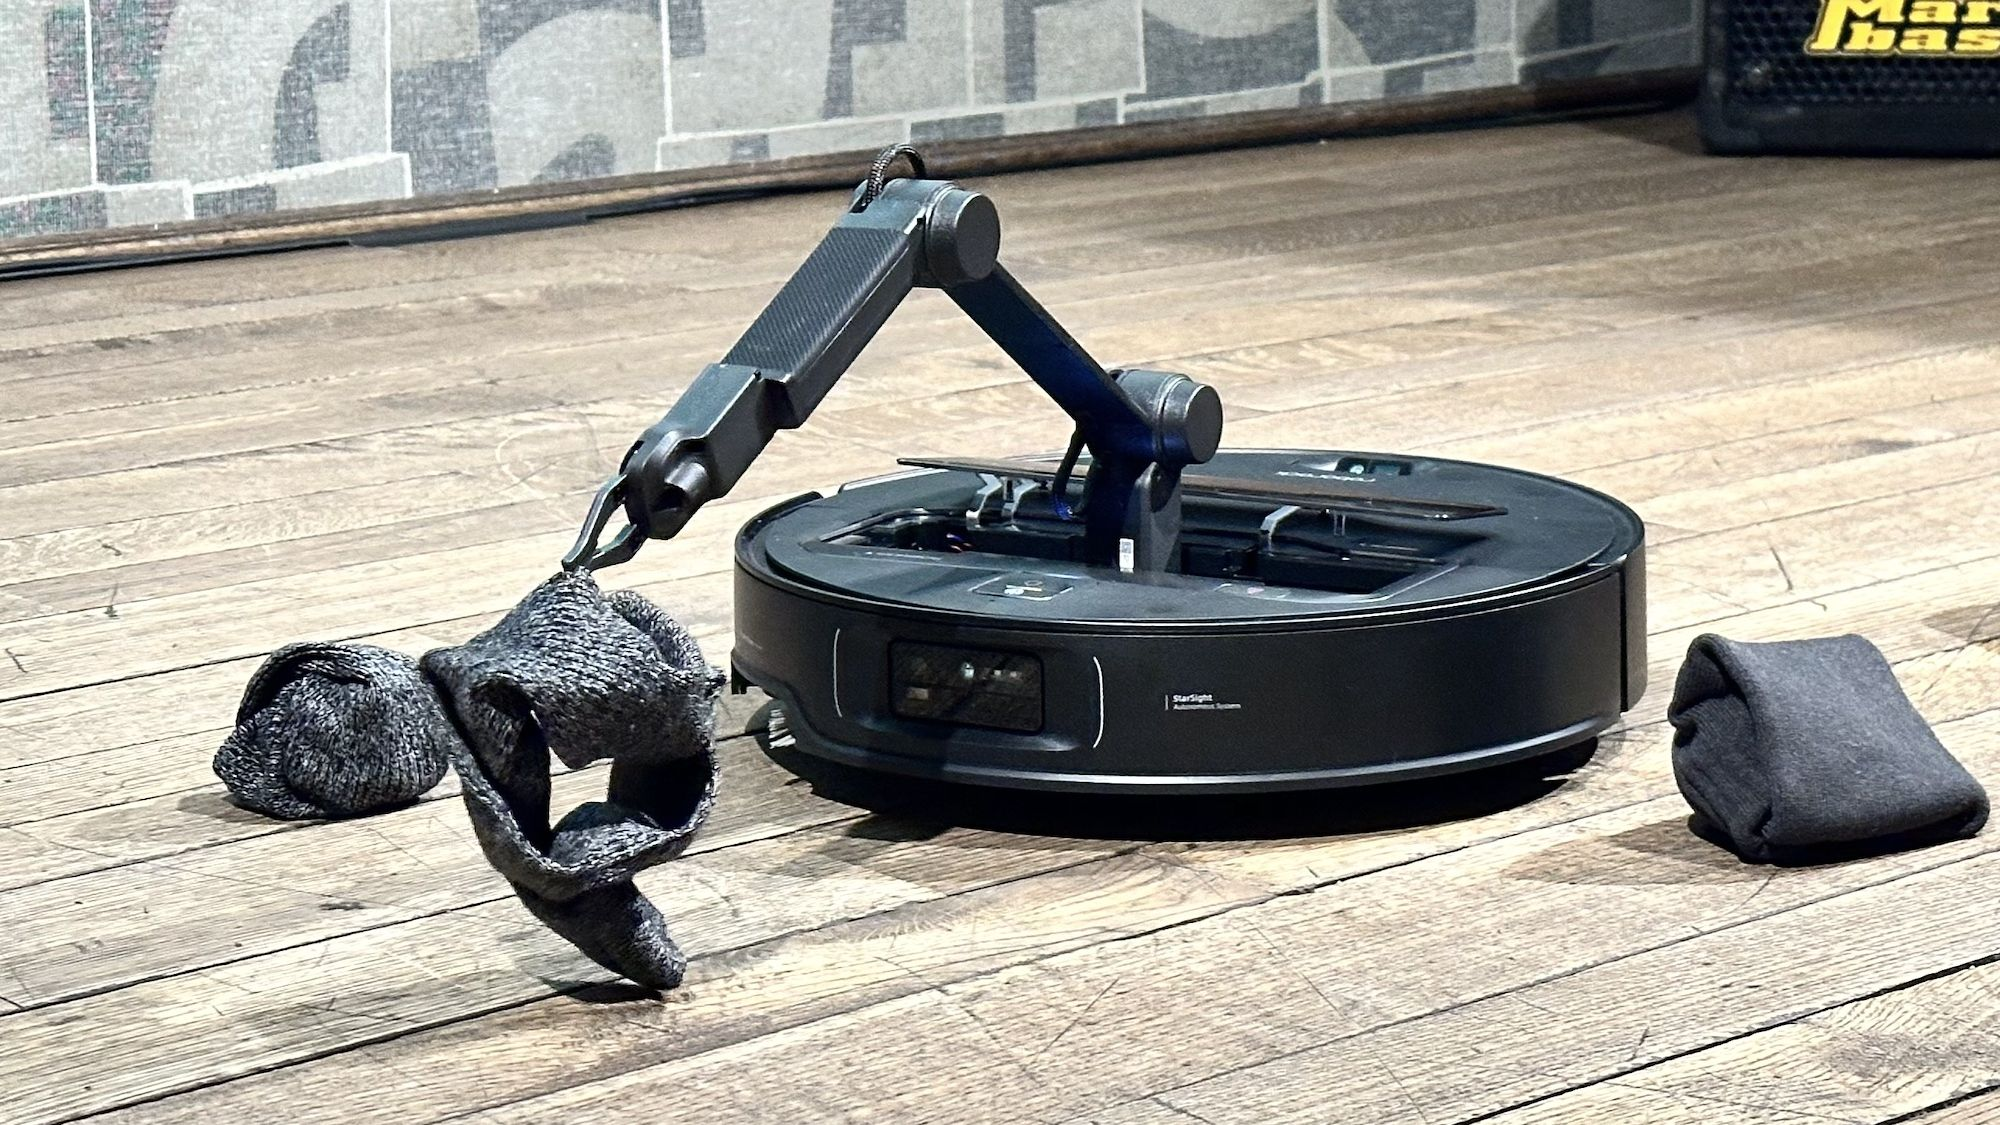
\includegraphics[width=0.6\textwidth]{figures/vacuum-cleaner.jpg}
\caption{Modern robotic vacuum cleaners utilize SLAM and localization technologies to autonomously navigate residential spaces, representing the most successful consumer robotics application to date.}
\label{fig:vacuum}
\end{figure}

The key to their success lies in the sophisticated implementation of SLAM (Simultaneous Localization and Mapping) and localization technologies. Modern robotic vacuum cleaners employ LiDAR sensors (Light Detection and Ranging), visual SLAM (VSLAM), and advanced mapping algorithms to create real-time maps of residential environments, enabling efficient path planning and obstacle avoidance \cite{neato2025}. This technology has proven so reliable that robotic vacuums have achieved nearly 40\% of the service robot market share \cite{trendforce2024}, demonstrating that autonomous navigation, when properly implemented, is mature enough for widespread consumer adoption.

    \item \textbf{Industrial Market: Amazon's Warehouse Robotics Dominance.}\newline
    In the industrial sector, the most successful large-scale application of AMRs (Autonomous Mobile Robots) has been warehouse automation, with Amazon leading the field. Amazon reports more than 750,000 to over one million robots across its fulfillment network, including drive units, mobile manipulators, and next-generation platforms such as Pegasus and Xanthus \cite{amazon2024ai, amazon2022}. These fleets demonstrate reliable fleet management, safe human–robot collaboration, and 24/7 uptime in highly dynamic environments.

\begin{figure}[H]
\centering
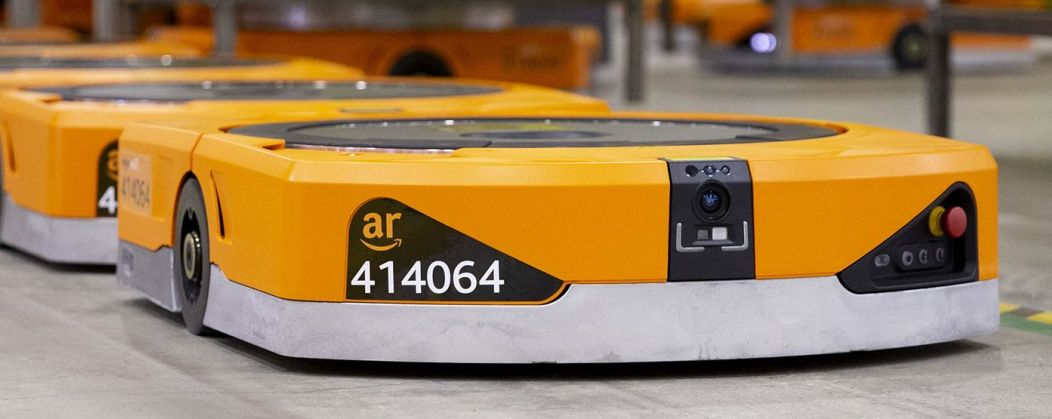
\includegraphics[width=0.9\textwidth]{figures/Amazon-Pegasus.jpg}
\caption{Amazon Pegasus drive unit used in high-throughput fulfillment centers.}
\label{fig:amazon-pegasus}
\end{figure}

    \item \textbf{Quadruped Robotics: Unitree Go2 as a Robust Mobility Platform.}\newline
    State-of-the-art quadruped robots such as Unitree Go2 demonstrate robust mobility on unpredictable terrain using reinforcement learning for locomotion policy optimization, advanced multi-sensor perception (3D LiDAR + depth/RGB cameras), and high-performance onboard compute for real-time planning and control. These capabilities enable operation on stairs, slopes, and uneven surfaces, with compelling applications in inspection, security, and emergency response \cite{unitreeGo2spec, unitreeRL2024}. Although not our primary target platform, Unitree’s capabilities illustrate complementary directions for rugged environments using RL and advanced multi-sensor perception, and inspire future extensions. 

\begin{figure}[H]
\centering
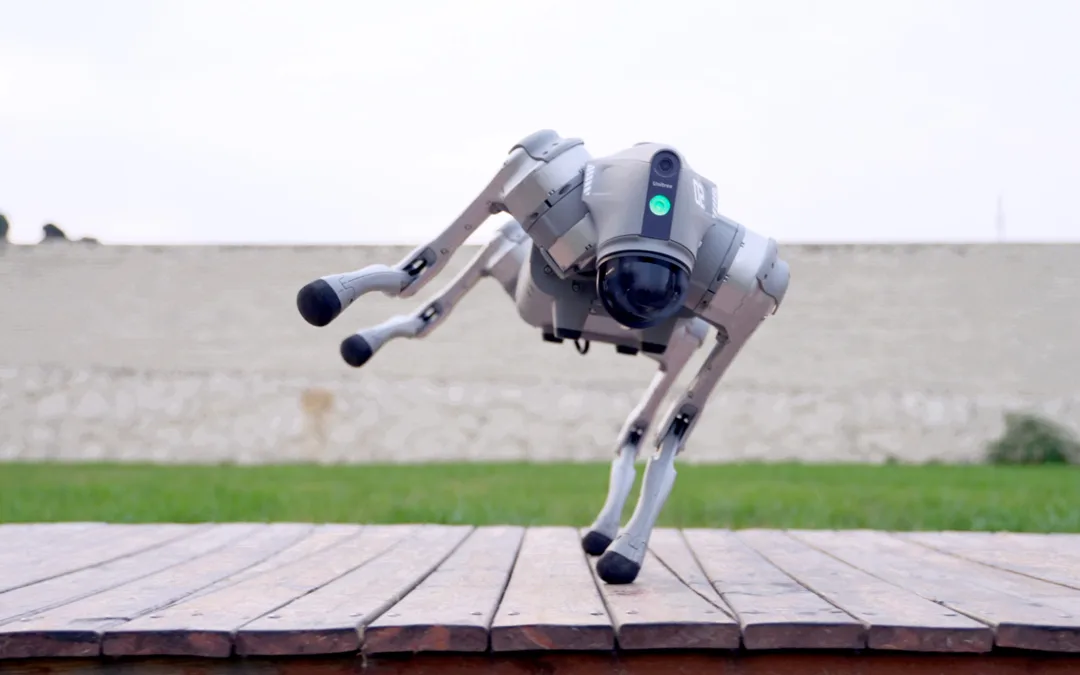
\includegraphics[width=0.9\textwidth]{figures/Unitree-Go2-6-copy-1080x675.png}
\caption{Unitree Go2: quadruped platform featuring RL locomotion, multi-sensor perception, and high-performance compute.}
\label{fig:unitree-go2}
\end{figure}
\end{enumerate}

\subsubsection{Benefits of Autonomous Mobile Robots in Healthcare Settings}

Recent literature and deployment data reveal multiple evidence-based benefits of AMRs in hospital environments:

\paragraph{Infection Control and Reduced Human Contact.}
AMRs significantly minimize human-to-human contact, reducing cross-contamination risks a critical advantage demonstrated during the COVID-19 pandemic \cite{intel2024, frontiers2024}. Autonomous delivery robots eliminate the need for multiple staff members to handle potentially contaminated materials, reducing occupational exposure and conserving personal protective equipment. UV-C (ultraviolet-C) disinfection robots have been shown to achieve 99.9\% pathogen kill rates on environmental surfaces, helping reduce hospital-acquired infections (HAIs) \cite{sciencedirect2021}.

\paragraph{Wayfinding and Visitor Guidance.}
Intelligent hospital guidance robots provide accurate navigation assistance to visitors and patients, reducing confusion and staff burden \cite{pmc2024nursing}. These robots can escort visitors to patient rooms, provide multilingual directions, and answer frequently asked questions about hospital facilities, allowing staff to focus on clinical care.

\paragraph{Material Transport and Delivery.}
AMRs excel at routine delivery tasks including medications, meals, linens, laboratory specimens, and medical supplies. This automation frees nursing staff from non-clinical transport duties, allowing them to spend more time on direct patient care. Studies indicate that delivery robots can reduce staff time spent on logistics by up to 30\% \cite{mdpi2024}.

\paragraph{Psychological Support and Patient Morale.}
Research consistently demonstrates that pediatric patients exhibit positive emotional responses to robot interactions \cite{beran2013}. Socially interactive robots reduce anxiety, provide distraction during painful procedures, and improve treatment compliance in children. Studies show that patients perceive robotic companions as non-judgemental, reducing psychological barriers to seeking help or expressing concerns \cite{ahu2024}.

\paragraph{Autonomous Disinfection and Cleaning.}
Cleaning and disinfection robots can be equipped with UV-C light systems at relatively low cost, providing continuous environmental sanitation \cite{intel2024}. These robots operate during off-peak hours without human supervision, ensuring consistent hygiene standards while minimizing disruption to clinical workflows.

\paragraph{Telepresence and Virtual Presence.}
AMRs with integrated telepresence capabilities enable remote consultations, family visits, and specialist rounds without requiring travel \cite{garingo2016}. This technology proved invaluable during pandemic restrictions and continues to provide value for rural healthcare access and specialist consultations.

\paragraph{Waste Collection and Handling.}
Some advanced AMR systems are deployed for biohazardous waste collection and disposal, reducing staff exposure to potentially infectious materials \cite{mdpi2024}. In China and other Asian markets, robots have been successfully implemented for collecting and transporting medical waste from patient rooms to centralized disposal areas, demonstrating significant improvements in operational efficiency and staff safety.

\subsubsection{Challenges in Hospital AMR Deployment}

Despite the significant benefits, several challenges remain:

\paragraph{Cost and Return on Investment.}
Hospital-grade AMRs represent substantial capital investments, typically ranging from \$50,000 to \$150,000 per unit depending on capabilities. Healthcare administrators require clear Return on Investment (ROI) demonstration through labor savings, efficiency gains, and improved outcomes to justify procurement \cite{mdpi2024}.

\paragraph{System Integration Complexity.}
Integrating AMRs with existing hospital information systems (HIS), electronic health records (EHR), elevator controls, automatic doors, and staff communication systems presents significant technical challenges. Interoperability standards are still evolving, requiring custom integration work for each deployment \cite{frontiers2024}.

\paragraph{Safety, Privacy, and Trust.}
Regulatory compliance (HIPAA, GDPR), patient data security, and physical safety in crowded environments remain critical concerns. Healthcare facilities must ensure that robots can safely navigate around patients, visitors, and medical equipment while maintaining patient privacy and data security \cite{jmir2024}. Building trust among staff and patients requires careful change management and demonstration of reliability.

\paragraph{Regulatory and Liability Issues.}
Medical device regulations, liability frameworks for autonomous systems, and insurance considerations create additional barriers to widespread adoption. Healthcare organizations must navigate complex approval processes and establish clear accountability frameworks for robot operations.

\subsubsection{Overview of Existing Robots in Healthcare}
The hospital robotics market has matured significantly, with several manufacturers deploying autonomous mobile robots at scale. Table~\ref{tab:competitive} presents a comprehensive comparison of leading hospital robot platforms currently deployed in eastern markets. Note that prices are approximate estimates and can vary significantly depending on region, configuration, volume, and additional features.

\begin{table}[H]
\centering
\small
\begin{tabular}{|l|p{2.5cm}|p{2cm}|p{1.5cm}|p{2.5cm}|p{4cm}|}
\hline
    \textbf{Rank} & \textbf{Manufacturer \& Model} & \textbf{Est. Deploy-ments} & \textbf{Est. Price (USD)} & \textbf{Key Hospital Applications} & \textbf{Features \& Notes} \\
\hline
1 & Pudu Robotics – PuduBot 2 \cite{pudubot2} & 15,000–20,000 units (~5,000 healthcare) & ~\$12,000 & Medication/meal delivery, linen transport, waste collection & Multi-floor navigation (elevator integration), VSLAM+LiDAR, 40 kg payload, 6–8 hr battery. Deployed in 100+ hospitals globally (China, Singapore, U.S.); customizable trays, infection-resistant coating. \\
\hline
2 & Keenon Robotics – M2 Medical Robot \cite{m2medical} & 8,000–10,000 units (healthcare-focused) & ~\$47,500 & UV-C disinfection, medication/lab sample delivery, patient room cleaning & UV sterilization (99.9\% pathogen kill rate), 40 kg payload, voice interaction, 10 hr runtime. Used in 100+ Chinese hospitals during COVID; exported to U.S./Europe (HIPAA-compliant). \\
\hline
3 & Pudu Robotics – PUDU CC1 \cite{puducc1} & 5,000–7,000 units (healthcare + hospitality) & ~\$16,800 & Floor cleaning, disinfection, material transport & Autonomous scrubbing (1,500 m²/hr), self-charging, obstacle avoidance. Popular in Chinese/U.S. hospitals for large-scale sanitation; integrates with PuduBot for hybrid tasks. \\
\hline
4 & Keenon Robotics – Peanut Medical \cite{peanutmedical} & 3,000–5,000 units & ~\$12,700 & Medication/meal delivery, patient guidance, telepresence & Compact (59 cm wide), multi-modal navigation, 30 kg payload. Deployed in Asia-Pacific hospitals; supports remote doctor-patient interaction via screen. \\
\hline
\end{tabular}
\caption{Competitive analysis of leading hospital AMR platforms by global deployment and capabilities.}
\label{tab:competitive}
\end{table}

\begin{figure}[H]
\centering
\begin{minipage}{0.45\textwidth}
\centering
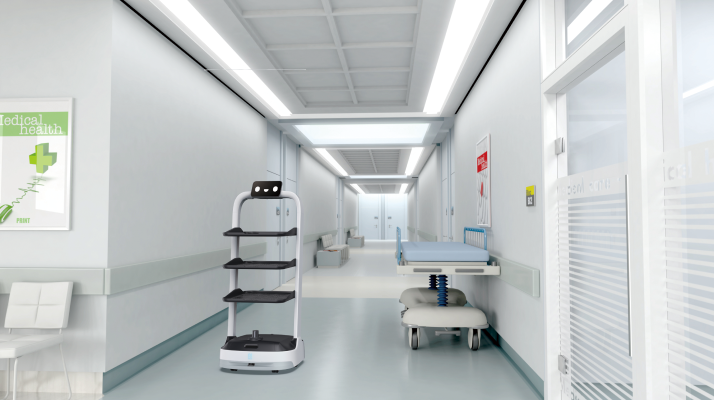
\includegraphics[width=\textwidth]{figures/pudubot-sante.png}
\caption{Pudu Robotics PuduBot 2}
\label{fig:pudubot}
\end{minipage}\hfill
\begin{minipage}{0.45\textwidth}
\centering
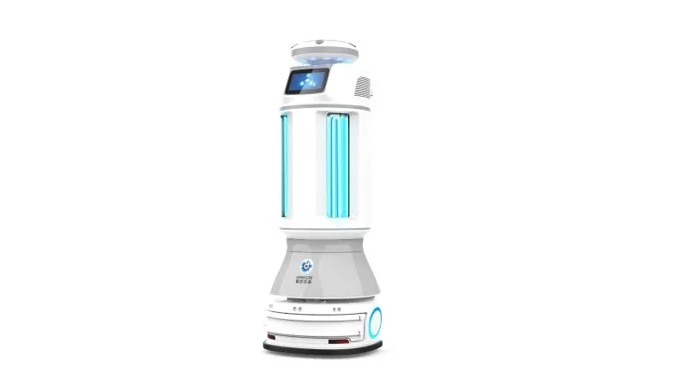
\includegraphics[width=\textwidth]{figures/KEENON-M2-Disinfection-Robot.jpg}
\caption{Keenon M2 Medical Robot}
\end{minipage}

\vspace{0.5cm}

\begin{minipage}{0.45\textwidth}
\centering
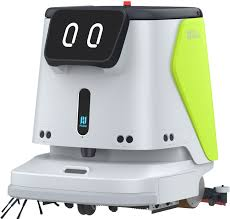
\includegraphics[width=\textwidth]{figures/pudu-cc1.jpeg}
\caption{Pudu Robotics PUDU CC1}
\label{fig:cc1}
\end{minipage}\hfill
\begin{minipage}{0.45\textwidth}
\centering
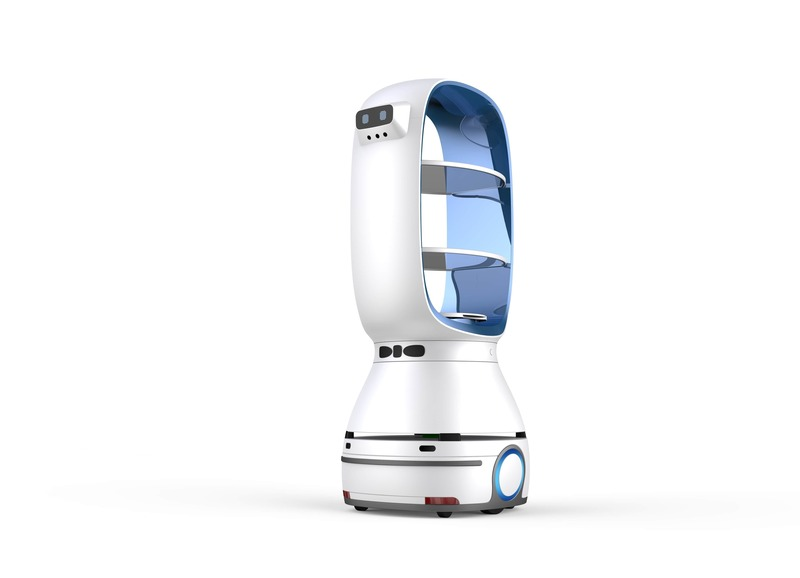
\includegraphics[width=\textwidth]{figures/peanut.jpg}
\caption{Keenon Peanut Medical}
\label{fig:peanut}
\end{minipage}
\end{figure}

In parallel, the field of Socially Assistive Robotics (SAR) has focused on the psycho-social aspects of patient care. These robots are designed not to perform physical tasks but to engage, encourage, and comfort patients through social interaction. For pediatric patients, robots like NAO and PARO (a therapeutic baby seal robot) have been shown to significantly reduce pain perception and anxiety during painful medical procedures such as vaccinations and chemotherapy \cite{beran2013}. The robot acts as a coach and a distractor, creating a more positive and cooperative atmosphere. For elderly populations, SARs have been explored for companionship to combat loneliness, provide cognitive stimulation for dementia patients, and deliver medication reminders to improve treatment adherence \cite{broekens2009}. These studies confirm that a robot's ability to interact socially is a powerful tool for improving patient well-being and clinical outcomes. The primary limitation of SARs, however, is that they are typically specialized, non-mobile or semi-autonomous platforms that lack the high-fidelity telepresence capabilities needed for direct clinical consultation.

\subsection{Technical Building Blocks}
This section deconstructs the essential technologies that form the foundation of an advanced autonomous healthcare robot. It examines navigation systems including Radio Frequency (RF) localization and SLAM-based sensor fusion, mobile robot platform specifications and selection criteria, Conversational AI and Large Language Models (LLMs) for intelligent interaction, and User Interface (UI) and Human-Robot Interaction (HRI) design paradigms for clinical integration.

\subsubsection{Navigation System}
The challenge of manual navigation highlighted in telepresence research is being addressed by autonomous mobile robots (AMRs). Modern AMRs employ a combination of SLAM, path planning, and obstacle avoidance to navigate complex environments without human intervention. The core navigation stack typically includes Radio Frequency (RF) Localization Technologies and SLAM-Based Sensor Fusion Techniques.

\paragraph{Radio Frequency (RF) Localization Technologies}
Radio frequency (RF) refers to electromagnetic waves (3 kHz--300 GHz) used for wireless communication. RF-based localization is essential where GPS is unreliable, such as indoors or through obstacles. Technologies like Wi-Fi, RFID, Bluetooth Low Energy (BLE), ZigBee, and Ultra-Wideband (UWB) are used, each selected based on coverage, scalability, battery life, accuracy, and cost. UWB, for example, enables multi-node scalability and multi-year tag battery life, but at higher cost (e.g., up to \$20,000 for a 5000~m$^2$ facility). Accuracy ranges from about 20~cm to over 1~m, with performance degrading in cluttered or metallic environments \cite{chen2022}. The general structure of these systems is to use static reference sensor locations, or anchors, within an environment, along with beacons or tags fixed to the objects with desired tracking. The location of the tracked object can be estimated using readings from the anchors. Mathematically, this estimation is commonly called multilateration (also called trilateration) when using distance measurements. Figure~\ref{fig:uwb} shows an example UWB anchor--tag geometry, while figure~\ref{fig:multilateration} illustrates the multilateration technique.
\begin{figure}[H]
\centering
\begin{minipage}{0.45\textwidth}
\centering
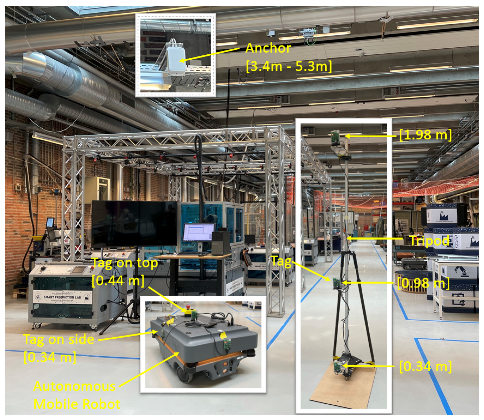
\includegraphics[width=\textwidth]{figures/uwb.png}
\caption{UWB anchor--tag geometry for ranging and multilateration-based localization in indoor environments.}
\label{fig:uwb}
\end{minipage}\hfill
\begin{minipage}{0.50\textwidth}
\centering
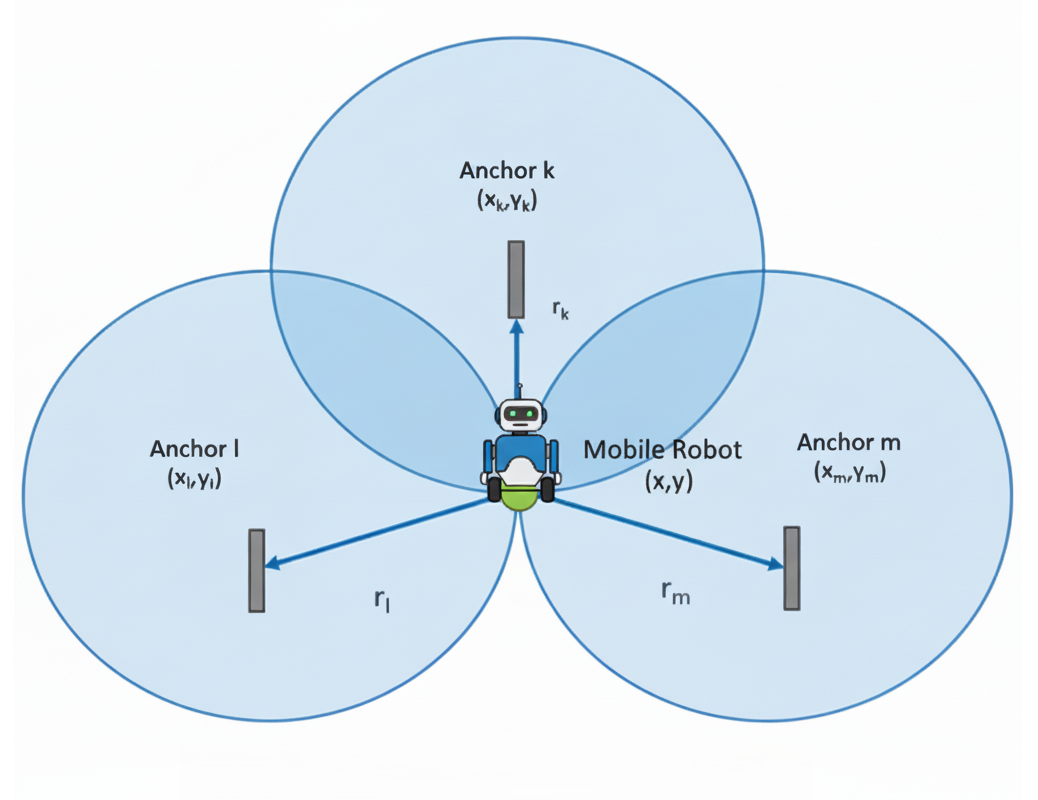
\includegraphics[width=\textwidth]{figures/Multilateration.png}
\caption{Illustration of multilateration technique. Each known anchor forms a circle with radius equal to its distance to the robot, and the robot’s estimated position is where these circles intersect.}
\label{fig:multilateration}
\end{minipage}
\end{figure}
Angle of Arrival (AoA) is a localization technique that determines the direction or angle from which a radio signal is received. An antenna array senses time differences across elements and applies signal-processing algorithms such as MUSIC or ESPRIT to convert those differences into an angle. AoA (often via BLE 5.1+ or UWB Direction Finding) estimates a target's angle using a beacon or tag and a robot-mounted antenna array, reducing reliance on dense static infrastructure. BLE-based tags offer excellent battery life (years). Limitations include line-of-sight sensitivity and variable accuracy; hybrid AoA + RSSI filtering can improve precision, achieving mean errors on the order of 12 cm in simulation even in cluttered settings \cite{weinmann2023}. AoA could be used to implement a solution that does not depend on localization or positioning infrastructure in the environment, instead having the robot home in on a beacon worn by the user. This would be similar to how some Bluetooth trackers work for finding lost items. The robot would use the angle of arrival data to determine the direction to move towards the beacon signal, allowing it to autonomously navigate to the user's location. This approach could be particularly useful in dynamic environments like hospitals where fixed infrastructure may not be feasible. Figure~\ref{fig:amr-stack} illustrates a proposed setup where a Bluetooth homing controller on the robot uses AoA data from a wearable beacon to guide navigation towards the target. Multiple anchors could be used to implement waypoints following navigation paths through the environment. 

\begin{figure}[H]
\centering
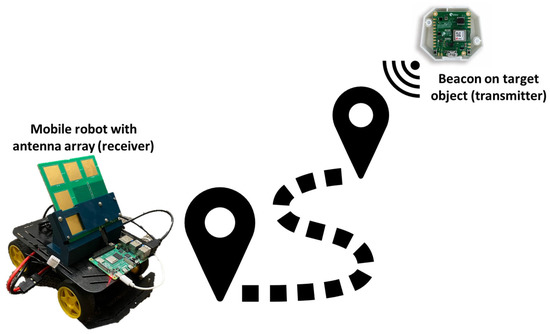
\includegraphics[width=0.5\textwidth]{figures/config.jpg}
\caption{Configuration of proposed setup of Bluetooth homing controller.}
\label{fig:amr-stack}
\end{figure}

\paragraph{SLAM-Based Sensor Fusion Techniques}
Simultaneous Localization and Mapping (SLAM) is a critical technology for autonomous navigation, enabling robots to build maps of unknown environments while simultaneously keeping track of their own location. Its effectiveness hinges on robust sensor fusion techniques that integrate data from various sources such as camera(s), IMU, wheel odometry, or RF ranging. Beyond external RF systems, autonomous navigation heavily relies on SLAM with multi-sensor fusion for robustness. A common stack fuses 2D LiDAR with an IMU and wheel odometry. IMU and odometry constrain motion, correcting LiDAR motion distortion and mitigating slip-induced drift. Studies report substantial gains when integrating IMU and wheel odometry, for example, approximately 27\% improvement in rotation error and greater than 67\% reduction in position error relative to LiDAR only SLAM, at the expense of added system complexity and compute \cite{doduc2024}.

VSLAM (Visual Simultaneous Localization and Mapping) is a method that uses cameras to help robots figure out where they are and build maps of their surroundings at the same time. VSLAM uses cameras like monocular (single), stereo (two), or RGB-D (depth-sensing) for positioning and mapping. It provides low-cost, lightweight hardware and better scene understanding. Challenges include poor performance in texture-less or repetitive areas, and scale issues in monocular systems (e.g., early ORB-SLAM 2.0). Modern approaches prefer hybrid Visual–Inertial–Ranging–LiDAR (VIRAL) SLAM for improved reliability in complex environments \cite{tourani2022}. Figure~\ref{fig:slam} shows the combination of visual/laser data with inertial and odometric inputs for stable estimation. Tools like Google Cartographer build 3D maps in real-time, using LiDAR, IMU, and odometry. 
\begin{figure}[H]
\centering
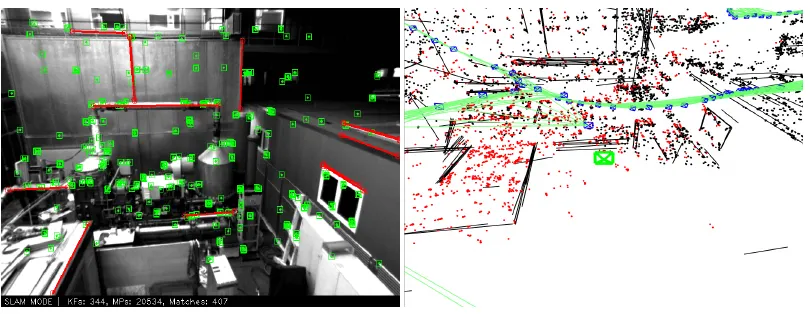
\includegraphics[width=0.75\textwidth]{figures/slam.png}
\caption{Illustration of SLAM fusion: visual/laser perception integrated with inertial and odometric constraints for robust state estimation.}
\label{fig:slam}
\end{figure}

\paragraph{Navigation Systems Across Hospital Robotics Platforms.}
Table~\ref{tab:robot_nav} summarizes the navigation technologies and sensor configurations employed by leading hospital robotics platforms mentioned in table \ref{tab:competitive}.

\begin{table}[H]
\centering
\small
\begin{tabular}{|l|p{2.5cm}|p{2.5cm}|p{3.5cm}|}
\hline
\textbf{Robot Model} & \textbf{Primary Localization} & \textbf{Mapping Technology} & \textbf{Key Sensors} \\
\hline
PuduBot 2 \cite{pudubot2} & SLAM (LiDAR-based) & Real-time 2D/3D mapping & 2D LiDAR, depth camera, IMU \\
\hline
M2 Medical Robot \cite{m2medical} & SLAM (LiDAR-based) & Real-time 2D mapping & 2D LiDAR, RGB camera, encoders \\
\hline
PUDU CC1 \cite{puducc1} & SLAM (LiDAR-based) & Real-time 2D mapping & 2D LiDAR, ultrasonic sensors, encoders \\
\hline
Peanut Medical \cite{peanutmedical} & Hybrid (SLAM + RF) & Real-time 2D mapping & LiDAR, depth sensors, optional UWB \\
\hline
\end{tabular}
\caption{Navigation systems and sensor technologies across leading hospital robotics platforms.}
\label{tab:robot_nav}
\end{table}

\subsubsection{Mobile Robot Platform specifications}

The selection of an appropriate mobile robot platform is a critical decision that directly impacts system reliability, development time, and operational costs. For a healthcare telepresence robot operating in hospital corridors and patient rooms, the platform must satisfy several essential technical and operational requirements while remaining within practical budget constraints.

\paragraph{Platform Requirements.}
The system requires a wheeled mobile robot platform with the following capabilities:

\begin{itemize}[leftmargin=*]
    \item \textbf{Autonomous docking and charging} with high-level API commands (\texttt{dock()}, \texttt{return\_to\_charge()})
    \item \textbf{ROS/ROS 2 compatibility} for navigation packages (Nav2, SLAM Toolbox, AMCL)
    \item \textbf{Payload capacity} of 5--10~kg for telepresence screen, onboard computer, and camera system
    \item \textbf{Indoor navigation sensors} including LiDAR (2D or 3D) and depth cameras
    \item \textbf{Safety and reliability} features (cliff detection, bumpers, emergency stop)
\end{itemize}

\paragraph{Project Constraints.}
Budget constraints significantly influence platform selection. The target budget for the mobile base, charging dock, and core sensors is approximately \$1,000--\$1,500 USD, recognizing that higher-cost industrial platforms (\$5,000+) exceed the scope of an educational research project. Additional constraints include global availability (shipping to Oman), vendor support and documentation quality, and community resources for troubleshooting and development.

\paragraph{Platform Comparison.}
Table~\ref{tab:platforms} presents a comparative analysis of commercially available mobile robot platforms. 

\begin{table}[H]
\centering
\footnotesize
\begin{tabular}{|p{3.2cm}|l|c|c|c|p{4.5cm}|}
\hline
\textbf{Platform} & \textbf{Price (USD)} & \textbf{Dock} & \textbf{ROS} & \textbf{Payload} & \textbf{Notes} \\
\hline
\multicolumn{6}{|c|}{\textit{Budget Tier (\$500--\$1,000)}} \\
\hline
iRobot Create 3 \cite{irobot2024create3} & \$549 & Yes & ROS 2 & 9~kg & Roomba-based, proven docking, ideal for education \\
\hline
Yahboom ROSMASTER X3 \cite{yahboom2024} & \$699 & DIY & ROS 1 & 5--8~kg & Mecanum wheels, requires custom docking solution \\
\hline
Elephant Robotics MyAGV 2023 \cite{elephantrobotics2024} & \$899 & DIY & ROS 1 & 8~kg & Mecanum wheels, 2D SLAM ready, Python/ROS compatible \\
\hline
\multicolumn{6}{|c|}{\textit{Mid-Tier (\$1,000--\$2,000)}} \\
\hline
SLAMTEC Apollo \cite{slamtec2024} & \$1,200 & Yes & ROS 1/2 & 50~kg & Same platform as Pudu/Keenon hospital robots \\
\hline
TurtleBot 4 Standard \cite{turtlebot2024} & \$1,400 & Yes & ROS 2 & 9~kg & Research-grade, Nav2 pre-configured, Lidar included \\
\hline
Husarion ROSbot 2R \cite{husarion2024} & \$1,600 & Optional & ROS 2 & 10~kg & Mecanum wheels, hospital navigation demos available \\
\hline
AgileX LIMO Pro \cite{agilex2024} & \$1,799 & Optional & ROS 2 & 10~kg & 4-mode steering, Jetson Nano, research platform \\
\hline
\end{tabular}
\caption{Comparative analysis of mobile robot platforms for healthcare telepresence applications.}
\label{tab:platforms}
\end{table}


\subsubsection{Conversational AI and Large Language Models (LLMs)}
\label{sec:llm}
The field of large language models (LLMs) has witnessed transformative advancements, establishing them as a core technology for conversational AI. An LLM is a sophisticated artificial intelligence system trained on vast datasets of text and code, enabling it to understand, generate, and interact with human language in a nuanced manner. These models have rapidly transitioned from research prototypes to industrial-scale technologies, resulting in a proliferation of models with distinct strengths and commercial terms.

The LLM landscape is broadly divided into two categories: open-source and proprietary. Open-source models, such as Meta's Llama series and the DeepSeek series, offer significant flexibility, allowing for deep customization and fine-tuning to meet specific application needs, often at a lower cost \cite{civo2024}. However, they may require more complex setup and can sometimes lag behind proprietary counterparts in raw performance. In contrast, privately-owned models like OpenAI's GPT series and Google's Gemini series typically offer state-of-the-art performance and are adept at handling highly complex tasks. This performance comes with trade-offs, including higher operational costs and potential data privacy concerns, which are critical considerations in healthcare applications \cite{musick2025}. The selection of an LLM depends on a careful balance between performance requirements, budget, customizability, and data governance policies. Table~\ref{tab:llm_comparison} provides a comparative overview of leading LLM options.

\begin{table}[H]
\centering
\small
% Use tabularx to make the table fit the text width. X columns will wrap text.
% The >{\...} commands are for text alignment within the columns.
\begin{tabularx}{\textwidth}{| >{\raggedright\arraybackslash}X | l | >{\raggedright\arraybackslash}X | >{\centering\arraybackslash}X | >{\centering\arraybackslash}X | >{\centering\arraybackslash}X |}
\hline
\textbf{Model (Version)} & \textbf{Org.} & \textbf{License} & \textbf{Max Context (tokens)} & \textbf{Input API Cost (\$/M)} & \textbf{Output API Cost (\$/M)} \\
\hline
OpenAI GPT-5.2 \cite{openai2025pricing} & OpenAI & Proprietary & 128,000 & \$1.75 & \$14.00 \\
\hline
Google Gemini 3 Flash \cite{google2025pricing} & Google & Proprietary & 1,000,000 & \$0.50 & \$3.00 \\
\hline
Google Gemini 2.5 Pro \cite{google2025pricing} & Google & Proprietary & 1,000,000 & \$1.25--\$2.50 & \$10.00--\$15.00 \\
\hline
Google Med-Gemma 2B & Google & Open Weight (Apache 2.0) & 8,192 & \$0.00 (Self-hosted) & \$0.00 (Self-hosted) \\
\hline
Meta Llama 4 Maverick \cite{llama2025} & Meta & Llama Community License & 10,000,000 & \$0.19--\$0.49 & \$0.19--\$0.49 \\
\hline
DeepSeek V3.1 \cite{deepseek2025} & DeepSeek & MIT (Code) / DeepSeek Model & 128,000 & \$0.14 & \$0.28 \\
\hline
\end{tabularx}
\caption{Comparative analysis of leading Large Language Models with December 2025 pricing and specifications.}
\label{tab:llm_comparison}
\end{table}

\paragraph{LLM Discussion and Cost Considerations.}
Table~\ref{tab:llm_comparison} summarizes key characteristics of leading LLM options as of December 2025. OpenAI's GPT-5.2 offers strong performance with a 128k token context window at \$1.75/\$14.00 per million input/output tokens. Google's Gemini 3 Flash provides exceptional value with a 1M token context and competitive pricing at \$0.50/\$3.00, with free tier available for development (up to 500 requests per day). Google's Gemini 2.5 Pro offers higher capabilities for complex tasks at \$1.25--\$2.50 input and \$10.00--\$15.00 output per million tokens. Google's Med-Gemma represents a family of specialized open-weight models (available in 2B, 7B, and 27B parameter variants) fine-tuned specifically on medical literature, clinical guidelines, and healthcare datasets \cite{medgemini2024}. While Med-Gemma demonstrates state-of-the-art performance on medical benchmarks (MedQA, MedMCQA, PubMedQA) and would be highly relevant for advanced clinical decision support or medical question answering, it is considered overkill for the basic conversational interactions required in this project (patient guidance, wayfinding, simple information queries). Meta's Llama 4 Maverick stands out with an unprecedented 10M token context window and industry-leading cost efficiency (\$0.19--\$0.49 per million tokens), making it highly suitable for long-context healthcare applications. DeepSeek V3.1 offers the most economical option at \$0.14/\$0.28 per million tokens, particularly beneficial for cost-sensitive deployments. For this project's conversational requirements (patient guidance, wayfinding, simple information queries), either Gemini 3 Flash (free tier) or DeepSeek V3.1 (lowest cost) would be appropriate choices, with Llama 4 Maverick offering future-proof long-context capabilities if advanced document processing becomes necessary.

\subsubsection{User Interface and Human-Robot Interaction}
For autonomous healthcare robots operating in clinical environments, the user interface (UI) and human-robot interaction (HRI) design directly impacts adoption, user satisfaction, and clinical workflow integration. The interface must balance accessibility for diverse user groups (clinicians, administrative staff, patients) with robust control mechanisms suitable for dynamic hospital environments. Common UI paradigms employed in hospital robotics include:

\paragraph{Onboard Touchscreen Interface.}
A dedicated touchscreen mounted on the robot body provides direct, localized control and real-time status feedback. Common in systems like Pudu Robotics' PuduBot 2 and Keenon Robotics' M2 Medical Robot, these interfaces typically run Android OS and display navigation status, task queues, and emergency controls. Advantages include intuitive interaction without external devices and immediate feedback. Limitations include reliance on the robot's physical proximity and potential hygiene concerns in sterile environments \cite{m2medical}.

\paragraph{Mobile Application (iOS/Android).}
Native mobile applications running on clinicians' and administrators' smartphones or tablets enable remote operation and fleet monitoring from anywhere within hospital networks. This approach is ubiquitous across commercial systems (PuduBot 2, M2, Peanut Medical) and supports features such as route customization, real-time tracking, task scheduling, and status notifications. Mobile apps offer flexibility and integrate seamlessly with existing hospital workflows, though they require network connectivity and depend on user device management \cite{pudubot2}.

\paragraph{Web-Based Dashboard.}
Cloud-hosted or on-premises web portals provide centralized fleet management, historical analytics, and administrative controls for hospital operators and IT administrators. Systems like Keenon Robotics and Pudu Robotics include web dashboards for route optimization, performance metrics, and multi-robot coordination. Web interfaces support remote monitoring across multiple locations and facilitate integration with hospital information systems (HIS). Trade-offs include network dependency, data security considerations, and potential latency in real-time control \cite{puducc1}.

\paragraph{Voice Control and Natural Language Interfaces.}
Voice-based interaction leveraging conversational AI and LLMs (as discussed in Section~\ref{sec:llm}) represents an emerging paradigm for hands-free operation in clinical settings. Systems like Keenon's M2 support voice commands, allowing clinicians to interact with robots while maintaining hygiene and workflow continuity. Voice interfaces reduce cognitive load and support more natural, intuitive interactions, but require robust speech recognition, noise handling (hospital environments are loud), and contextual understanding \cite{musick2025}.

\paragraph{Hospital Integration via APIs.}
Integration with existing hospital IT infrastructure through RESTful APIs or DICOM/HL7 standards allows robots to receive task assignments directly from electronic health records (EHR) or hospital management systems. This approach minimizes manual input and ensures tasks are coordinated with clinical workflows. Examples include systems capable of receiving delivery requests directly from hospital pharmacies or labs \cite{puducc1}.

\paragraph{Robot UI Usage Across Hospital Platforms.}
Table~\ref{tab:robot_ui} summarizes the UI and interaction modalities employed by leading hospital robotics platforms, illustrating the diversity of approaches and trade-offs in current systems.

\begin{table}[H]
\centering
\small
\begin{tabular}{|l|p{2cm}|p{2.5cm}|p{2.5cm}|p{2.5cm}|}
\hline
\textbf{Robot Model} & \textbf{Onboard Screen} & \textbf{Mobile App} & \textbf{Web Dashboard} & \textbf{Voice/AI Interface} \\
\hline
PuduBot 2 \cite{pudubot2} & Android tablet & iOS/Android & Yes & Limited \\
\hline
M2 Medical Robot \cite{m2medical} & Android display & iOS/Android & Yes & Yes (voice control) \\
\hline
PUDU CC1 \cite{puducc1} & Android panel & iOS/Android & Yes & No \\
\hline
Peanut Medical \cite{peanutmedical} & Optional & iOS/Android & Yes & Limited \\
\hline
\end{tabular}
\caption{UI and interaction modalities across leading hospital robotics platforms.}
\label{tab:robot_ui}
\end{table}

\clearpage

\subsection{Conclusion}

The literature presents a clear picture:
\begin{enumerate}
    \item \textbf{Telepresence robots} are effective for remote diagnosis but are limited by manual control and an impersonal user experience.
    \item \textbf{Socially assistive robots} have proven their value in patient engagement and comfort but lack clinical telepresence and advanced mobility.
    \item \textbf{Autonomous mobile robots} have mastered navigation in hospitals but are used for logistics, not patient interaction.
    \item \textbf{Conversational AI} offers intelligent dialogue but lacks the physical embodiment needed for meaningful healthcare encounters.
    \item \textbf{Consumer and industrial robotics} have demonstrated that autonomous navigation technology is mature, reliable, and cost-effective for real-world deployment, as evidenced by millions of robotic vacuum cleaners in homes and over one million AMRs in Amazon warehouses.
    \item \textbf{Current hospital AMRs} are predominantly focused on material transport and disinfection, with limited integration of social interaction, advanced telepresence, and conversational AI capabilities.
\end{enumerate}

The critical research gap lies at the intersection of these domains. There is a demonstrable need for a single, integrated platform that combines the \textbf{clinical access} of a telepresence robot, the \textbf{patient-centric engagement} of a SAR, the \textbf{operational independence} of an autonomous navigator, and the \textbf{interactive intelligence} of modern conversational AI. The proven success of autonomous navigation in consumer (robotic vacuums) and industrial (Amazon warehouses) applications demonstrates that the core technology is mature and ready for advanced healthcare applications.

This project directly addresses this gap by designing a holistic system that synthesizes these strengths, creating a smart healthcare robot capable of not only connecting doctors and patients but also navigating its environment independently and engaging with patients in a helpful and empathetic manner. By learning from the successes of consumer robotics, warehouse automation, and existing hospital AMR deployments, this project aims to advance the state-of-the-art in healthcare robotics toward truly integrated, intelligent, and patient-centered care.

\clearpage


% Chapter 3: Requirements Specifications
\chapterintro{3}{Requirements Specifications}{This chapter defines customer and engineering requirements for the smart healthcare robot, establishing quantifiable specifications for navigation, telepresence, AI interaction, power management, and safety that guide system design and validation.}
\section{Requirements Specifications}
\label{sec:requirements}
\subsection{Introduction}

The success of any engineering project hinges on a clear, comprehensive understanding of the requirements that guide design, implementation, and evaluation. This chapter formalizes the requirement specification for the smart healthcare robot project, translating stakeholder needs and technical constraints into measurable, verifiable criteria. The requirements are systematically categorized into customer requirements, engineering requirements, and engineering constraints, ensuring alignment between user expectations and technical feasibility.

Customer requirements capture the high-level needs and expectations of primary stakeholders--hospital administrators, clinical staff, patients, and support personnel. These requirements reflect the functional and operational capabilities that directly impact system value and user satisfaction. Engineering requirements translate customer needs into quantifiable, testable technical specifications that guide system architecture and component selection. Engineering constraints define the boundaries within which the system must operate, including budget limitations, timeline restrictions, regulatory compliance, and environmental conditions specific to hospital deployment in Oman.

This chapter also presents a structured analysis of design alternatives, trade-offs, and selection criteria through comparative tables with metrics and scores. These analyses document the rationale for key architectural decisions, including mobile platform selection, sensor configuration, computing architecture, and AI integration strategy. The systematic evaluation ensures that design choices are transparent, justified, and optimized for the project's objectives and constraints.

By establishing a rigorous requirement framework, this chapter provides the foundation for subsequent design, implementation, and validation activities, ensuring that the final system meets stakeholder needs while remaining technically feasible and economically viable.

\subsection{Customer Requirements}

Customer requirements represent the high-level needs and expectations of the robot's primary users and stakeholders in hospital environments. These requirements are derived from literature review findings (Chapter 2), observations of existing hospital robotics deployments, and anticipated use cases in Omani healthcare facilities.

\begin{itemize}
    \item \textbf{CR1: Autonomous Navigation and Mobility.} The robot must autonomously navigate hospital corridors, patient rooms, and common areas without human intervention, avoiding static and dynamic obstacles. 
    
    \item \textbf{CR2: Remote Telepresence Capabilities.} The robot must enable high-quality remote video and audio communication between healthcare providers and patients, supporting remote consultations, rounds, and family visits. Telepresence has been validated as effective for remote diagnosis, specialist consultations, and reducing travel costs \cite{garingo2016}. The robot must provide a mobile "presence" for clinicians who are not physically at the patient's bedside.
    
    \item \textbf{CR3: Patient Engagement and Social Interaction.} The robot must engage with patients through natural language conversation, providing information, companionship, and emotional support, particularly for pediatric and elderly populations.
    
    \item \textbf{CR4: Infection Control and Hygiene.} The robot must be designed with materials and surfaces that are easy to clean and disinfect, minimizing cross-contamination risks. Hospital-acquired infections (HAIs) are a critical concern. Robots must be compatible with standard hospital cleaning protocols and potentially integrate UV-C disinfection capabilities \cite{intel2024, sciencedirect2021}.
    
    \item \textbf{CR5: User-Friendly Interface.} The robot must provide intuitive interfaces (touchscreen, mobile app, voice control) accessible to users with varying technical expertise. Ease of use directly impacts adoption rates and operational efficiency. Interfaces must accommodate diverse user groups including elderly patients, clinicians with minimal robotics experience, and administrative staff.
    
    \item \textbf{CR6: Continuous Operation and Autonomous Charging.} The robot must operate throughout the day with minimal downtime, autonomously returning to a charging dock when battery levels are low.
\end{itemize}

\subsection{Engineering Requirements}

Engineering requirements translate customer needs into quantifiable, testable technical specifications that directly inform system design and validation. Each engineering requirement is mapped to one or more customer requirements, ensuring traceability and alignment. The requirements are organized into five categories, presented in tabular format for clarity and traceability.

\subsubsection{Navigation and Mobility Requirements}

\begin{table}[H]
\centering
\small
\begin{tabularx}{\linewidth}{|l|>{\raggedright\arraybackslash}X|l|>{\raggedright\arraybackslash}X|>{\raggedright\arraybackslash}X|}
\hline
\textbf{Req. ID} & \textbf{Specification} & \textbf{Mapped to CR} & \textbf{Standards} & \textbf{Verification Method} \\
\hline
ER1.1 & Position accuracy of $\pm$20~cm in mapped indoor environments & CR1 & ISO 13482:2014 \cite{iso13482:2014} (Safety requirements for personal care robots - mobile servant robots) & Experimental validation using ground-truth positioning system \\
\hline
ER1.2 & Maximum linear velocity of 0.5--1.0~m/s in hospital corridors & CR1 & ISO 13482:2014 \cite{iso13482:2014} (Speed limits for safe human-robot interaction) & Speed measurement tests in controlled environments and hospital corridors \\
\hline
ER1.3 & Detect and avoid static and dynamic obstacles with minimum detection range of 3~m and reaction time $<$1~s & CR1 & ISO 13855 \cite{iso13855} (Safety of machinery - Positioning of safeguards) & Obstacle avoidance tests with various object types and approach angles \\
\hline
ER1.4 & Minimum payload of 5~kg to accommodate onboard computers, sensors, and delivery items & CR2 & --- & Load testing with representative payload configurations \\
\hline
\end{tabularx}
\caption{Navigation and mobility engineering requirements.}
\label{tab:er_navigation}
\end{table}

\subsubsection{Telepresence and Communication Requirements}

\begin{table}[H]
\centering
\small
\begin{tabularx}{\linewidth}{|l|>{\raggedright\arraybackslash}X|l|>{\raggedright\arraybackslash}X|>{\raggedright\arraybackslash}X|}
\hline
\textbf{Req. ID} & \textbf{Specification} & \textbf{Mapped to CR} & \textbf{Standards} & \textbf{Verification Method} \\
\hline
ER2.1 & Minimum 720p (1280$\times$720) video resolution at 30~fps & CR2 & ITU-T H.264 / H.265 \cite{itut_h264_h265} (Advanced Video Coding) & Video quality assessment tests under typical hospital lighting and network conditions \\
\hline
ER2.2 & Bidirectional audio communication with noise cancellation and echo reduction, maintaining intelligibility in hospital environments (ambient noise up to 70~dB) & CR2 & --- & Audio quality tests (speech intelligibility index, background noise rejection) \\
\hline
ER2.3 & End-to-end latency $<$200~ms over hospital Wi-Fi networks & CR2 & IEEE 802.11 \cite{ieee802.11} (Wi-Fi Standards) & Network performance testing and latency measurements \\
\hline
\end{tabularx}
\caption{Telepresence and communication engineering requirements.}
\label{tab:er_telepresence}
\end{table}

\subsubsection{Social Interaction and AI Requirements}

\begin{table}[H]
\centering
\small
\begin{tabularx}{\linewidth}{|l|>{\raggedright\arraybackslash}X|l|>{\raggedright\arraybackslash}X|>{\raggedright\arraybackslash}X|}
\hline
\textbf{Req. ID} & \textbf{Specification} & \textbf{Mapped to CR} & \textbf{Standards} & \textbf{Verification Method} \\
\hline
ER3.1 & Accurately interpret user intent in English and Arabic with $>$90\% accuracy for common healthcare queries & CR3 & --- & User testing with standardized query sets and intent classification metrics \\
\hline
ER3.2 & Generate conversational responses within 3~seconds of user input & CR3 & --- & Response latency measurements under typical operating conditions \\
\hline
ER3.3 & Speech recognition in hospital environments with word error rate (WER) $<$10\% & CR5 & --- & Speech recognition testing with diverse speakers and noise levels \\
\hline
\end{tabularx}
\caption{Social interaction and AI engineering requirements.}
\label{tab:er_ai}
\end{table}

\subsubsection{Power and Endurance Requirements}

\begin{table}[H]
\centering
\small
\begin{tabularx}{\linewidth}{|l|>{\raggedright\arraybackslash}X|l|>{\raggedright\arraybackslash}X|>{\raggedright\arraybackslash}X|}
\hline
\textbf{Req. ID} & \textbf{Specification} & \textbf{Mapped to CR} & \textbf{Standards} & \textbf{Verification Method} \\
\hline
ER4.1 & Continuous operation for minimum of 4--6~hours under typical usage (mixed navigation, telepresence, and idle states) & CR6 & --- & Endurance testing with simulated clinical workflows \\
\hline
ER4.2 & Autonomously locate and dock with charging station when battery level reaches 20\%, with 95\% success rate & CR6 & --- & Repeated docking trials under various initial positions and orientations \\
\hline
\end{tabularx}
\caption{Power and endurance engineering requirements.}
\label{tab:er_power}
\end{table}

\subsubsection{Safety and Reliability Requirements}

\begin{table}[H]
\centering
\small
\begin{tabularx}{\linewidth}{|l|>{\raggedright\arraybackslash}X|l|>{\raggedright\arraybackslash}X|>{\raggedright\arraybackslash}X|}
\hline
\textbf{Req. ID} & \textbf{Specification} & \textbf{Mapped to CR} & \textbf{Standards} & \textbf{Verification Method} \\
\hline
ER5.1 & Physical emergency stop button(s) and remote e-stop capability via software interface & CR1 & ISO 13850 \cite{iso13850} (Safety of machinery - Emergency stop function) & Functional testing of emergency stop mechanisms \\
\hline
ER5.2 & Detect and avoid stairs, ramps $>$15° incline, and drop-offs $>$2~cm & CR1 & --- & Edge detection tests on stairs and elevated platforms \\
\hline
ER5.3 & Achieve $>$95\% uptime during operational hours, excluding scheduled maintenance & CR6 & --- & Long-term reliability testing and failure logging \\
\hline
\end{tabularx}
\caption{Safety and reliability engineering requirements.}
\label{tab:er_safety}
\end{table}

\subsubsection{Comparative Performance Metrics}

This section presents quantitative performance data and trade-off metrics for critical system components. The data, derived from technical specifications and benchmark studies, provides the empirical basis for architectural decisions. Comprehensive mobile platform comparison metrics, including navigation capabilities, payload specifications, and integration features, are detailed in the literature review (Chapter 2, Section 2.3.2).

\paragraph{Navigation Sensor Performance}
Table~\ref{tab:sensor_metrics} compares the performance of different sensor modalities in typical hospital environments.

\begin{table}[H]
\centering
\scriptsize
\begin{tabularx}{\linewidth}{|>{\raggedright\arraybackslash}X|>{\raggedright\arraybackslash}X|c|c|c|c|c|}
\hline
\textbf{Sensor Type} & \textbf{Scenario} & \textbf{Range (m)} & \textbf{Accuracy (cm)} & \textbf{FOV (deg)} & \textbf{Power (W)} & \textbf{Cost (\$)} \\
\hline
2D LiDAR (RPLiDAR) \cite{rplidar2024} & Corridor (Static) & 12.0 & $\pm$1.0 & 360 & 1.5 & 100 \\
\hline
2D LiDAR (RPLiDAR) \cite{rplidar2024} & Waiting Room (Dynamic) & 10.0 & $\pm$2.5 & 360 & 1.5 & 100 \\
\hline
RGB-D (RealSense) \cite{realsense2024} & Corridor (Static) & 4.0 & $\pm$2.0 & 87$\times$58 & 3.5 & 250 \\
\hline
RGB-D (RealSense) \cite{realsense2024} & Waiting Room (Dynamic) & 3.5 & $\pm$4.0 & 87$\times$58 & 3.5 & 250 \\
\hline
3D LiDAR (Velodyne) \cite{velodyne2024} & Corridor (Static) & 100.0 & $\pm$2.0 & 360$\times$30 & 8.0 & 4000 \\
\hline
\end{tabularx}
\caption{Performance metrics of navigation sensors in static and dynamic scenarios.}
\label{tab:sensor_metrics}
\end{table}

\paragraph{Computing Platform Benchmarks}
Table~\ref{tab:compute_metrics} details the computational capabilities and power efficiency of candidate onboard computers.

\begin{table}[H]
\centering
\footnotesize
\begin{tabular}{|l|c|c|c|}
\hline
\textbf{Platform} & \textbf{CPU Perf.} & \textbf{Power (W)} & \textbf{Cost (\$)} \\
\hline
Raspberry Pi 5 \cite{raspberrypi2024} & High & 5--8 & 80 \\
Jetson Nano \cite{jetsonnano2024} & Medium & 5--10 & 150 \\
Jetson Orin Nano \cite{jetsonorin2024} & Very High & 7--15 & 499 \\
\hline
\end{tabular}
\caption{Computational performance and power consumption benchmarks for embedded platforms.}
\label{tab:compute_metrics}
\end{table}

\paragraph{Conversational AI Model Selection}
Detailed performance and cost metrics for Large Language Models (LLMs), including context handling capabilities and operational costs for cloud-based and local deployment strategies, are presented in the literature review (Chapter 2, Section 2.3.3). These metrics inform the AI architecture selection for patient engagement and conversational interaction requirements (ER3.1--ER3.3).

\subsection{Engineering Constraints}

Engineering constraints define the boundaries within which the system must be designed and operated. These constraints reflect real-world limitations in budget, timeline, technology maturity, regulatory environment, and deployment context specific to Oman.

\begin{itemize}
    \item \textbf{EC1: Budget Constraints.} Total system cost must not exceed \$2,500 USD, including mobile platform, sensors, computing hardware, and accessories. As an educational research project with limited funding, the system must demonstrate feasibility and functionality within academic budget constraints while remaining representative of scalable commercial solutions. This limits selection to budget and mid-tier commercial platforms; excludes high-end industrial robots; requires prioritization of essential features.
    
    \item \textbf{EC2: Development Timeline.} System design, implementation, and validation must be completed within one academic year (9--10 months). Final year project timeline constraints necessitate realistic scope and phased development approach. This requires prioritization of core functionalities (navigation, telepresence, basic AI); potential deferral of advanced features (UV-C disinfection, complex HIS integration) to future work.
    
    \item \textbf{EC3: Hospital Environment Compatibility.} The robot must operate safely in hospital environments with corridor widths $\geq$1.5~m, elevator access, and typical hospital flooring (tile, linoleum). Omani hospital infrastructure follows international standards with standard corridor dimensions and flooring materials. Robot base width limited to $<$60~cm; wheel system must handle smooth indoor surfaces; turning radius must accommodate corridor navigation.
    
    \item \textbf{EC4: Network Infrastructure.} The robot must operate on standard hospital Wi-Fi networks (802.11n/ac) without requiring dedicated network infrastructure. Deployment feasibility requires compatibility with existing IT infrastructure; hospitals cannot always support custom networking solutions. System must tolerate variable network quality, latency, and temporary disconnections; requires local processing capabilities for critical functions.
    
    \item \textbf{EC5: Regulatory and Privacy Compliance.} The system must comply with patient privacy requirements and avoid collection or storage of protected health information (PHI) without proper authorization. Healthcare robotics must respect patient privacy and data security regulations (similar to HIPAA/GDPR principles). No persistent storage of patient conversations or video recordings; encrypted communication channels; clear data handling policies.
    
    \item \textbf{EC6: User Expertise Level.} The system must be operable by users with minimal technical training (hospital staff, patients) without requiring robotics expertise. Clinical adoption depends on ease of use and minimal training burden. Intuitive UI design; pre-configured waypoints; automated error recovery; comprehensive user documentation.
    
    \item \textbf{EC7: Environmental Operating Conditions.} The robot must operate reliably in indoor environments with temperature range 18--28°C, humidity 30--60\%, and typical hospital lighting conditions. Hospital climate control maintains stable environmental conditions; sensors and electronics must function within this range. Standard commercial-grade components acceptable; no specialized environmental hardening required.
    
    \item \textbf{EC8: Maintenance and Spare Parts.} The robot must utilize commercially available, globally sourced components with accessible supply chains for replacement parts. Long-term operational viability requires availability of replacement components in Oman or via international suppliers. Preference for mainstream platforms (ROS 2, Raspberry Pi, common sensors) over proprietary or region-specific components.
\end{itemize}

\subsection{Analysis and Discussion}

This section examines the comparative performance metrics to identify key trade-offs and demonstrate standards compliance within the constraints of hospital deployment in Oman. The analysis focuses on component selection criteria that balance technical requirements with practical deployment considerations specific to the Omani healthcare context.

\subsubsection{Performance Metrics and Trade-off Analysis}

Table~\ref{tab:sensor_metrics} reveals fundamental trade-offs in sensor selection. Range capabilities vary from 3.5m to 100m with corresponding cost differences of 40$\times$ (\$100 to \$4000). Accuracy degrades significantly in dynamic hospital environments (2--2.5$\times$ degradation), affecting position accuracy requirement ER1.1. Power consumption ranges from 1.5W to 8W, directly impacting endurance requirement ER4.1. Field of view characteristics--360° planar, 87°$\times$58° 3D, and 360°$\times$30° volumetric--address different aspects of obstacle detection requirement ER1.3.

Table~\ref{tab:compute_metrics} demonstrates computational trade-offs where platform costs range from \$80 to \$499, consuming 3--20\% of total budget constraint EC1. Power envelopes remain similar (5--15W) across platforms, making computational capability rather than endurance the primary selection factor for supporting navigation, AI processing (ER3.1--ER3.3), and telepresence (ER2.1--ER2.3) requirements.

\subsubsection{Standards Compliance and Deployment Context}

Navigation and safety components satisfy ISO 13482:2014 \cite{iso13482:2014} requirements (position accuracy ER1.1, speed limits ER1.2, obstacle detection ER1.3), ISO 13850 \cite{iso13850} emergency stop guidelines, and ISO 13855 \cite{iso13855} safeguarding standards. Communication systems implement ITU-T H.264/H.265 \cite{itut_h264_h265} video coding and IEEE 802.11 \cite{ieee802.11} wireless protocols for interoperability with Omani hospital IT infrastructure.

Deployment constraints EC3--EC8 address Omani hospital realities: standard corridor dimensions ($\geq$1.5m) and flooring materials, existing Wi-Fi infrastructure (802.11n/ac), climate-controlled environments (18--28°C), component availability through international supply chains, privacy compliance aligned with HIPAA/GDPR principles, and budget/timeline limitations (\$2,500, 9--10 months). These constraints guide component selection to ensure technical feasibility and operational viability in the Omani healthcare context.

Detailed comparative analysis of mobile platforms, computing architectures, and conversational AI models is presented in the literature review (Chapter 2, Sections 2.3.2--2.3.3).

\subsection{Conclusion}

This chapter established a comprehensive requirement specification for the smart healthcare robot project, systematically translating stakeholder expectations into measurable, verifiable technical criteria. The requirements are organized into customer requirements, engineering requirements, and engineering constraints, defining the system's functional capabilities, performance targets, and operational boundaries.

Engineering requirements reference relevant international standards including ISO 13482:2014 (personal care robots), ISO 13855 and ISO 13850 (machinery safety), ITU-T H.264/H.265 (video coding), and IEEE 802.11 (wireless communications), establishing the regulatory framework for system validation. Engineering constraints reflect budget limitations, timeline restrictions, and regulatory compliance needs specific to Omani healthcare deployment.

The comparative performance analysis in Section 3.3.6 provided empirical data on component characteristics, while Section 3.5 examined trade-offs in the context of standards compliance and Omani deployment requirements. The requirement specification establishes the foundation for system design decisions detailed in subsequent chapters, with traceability ensuring design choices can be validated against stakeholder needs and technical constraints.


% Chapter 4: System Conceptual Design
\chapterintro{4}{System Conceptual Design}{This chapter presents the high-level system architecture of the smart healthcare robot, including functional decomposition, design alternatives analysis using AHP methodology, hardware and software selection justification, and detailed subsystem specifications.}
\section{System Conceptual Design}
\label{sec:design}


\subsection{Introduction: System Overview}
The proposed smart healthcare robot is a mobile, autonomous platform designed to assist hospital staff in routine, non-critical tasks while providing patients with an intuitive human--robot interaction (HRI) interface. The robot operates primarily in indoor clinical environments such as hospital wards, corridors, and waiting areas. Its main roles include autonomous navigation, safe obstacle avoidance, point-to-point delivery of small items, basic patient interaction via conversational AI, and remote telepresence capabilities for clinical staff.

From a functional perspective, the robot must be able to localize itself in the hospital environment, plan safe paths between waypoints, and react to dynamic obstacles such as people, trolleys, and doors. It should expose a user-friendly interface through a tablet and voice interaction for nurses, doctors, and patients to issue tasks or receive information. The system is conceived as a modular platform so that sensors, software modules, and interaction modalities can be extended in future iterations without major redesign.

The overall system architecture follows a layered approach consisting of:
\begin{itemize}
    \item \textbf{Mobile Base Layer}: Providing locomotion, payload mounting, and physical robustness
    \item \textbf{Computing and Control Layer}: High-level computer running ROS~2 and microcontroller for real-time motor control
    \item \textbf{Navigation and Perception Layer}: Sensors for localization, mapping, and obstacle detection
    \item \textbf{Intelligence Layer}: Large Language Model (LLM) for natural language understanding and HRI
    \item \textbf{Communication and Interface Layer}: Tablet UI, web dashboard, and voice interaction
    \item \textbf{Power Management Layer}: Battery system with automatic docking capabilities
\end{itemize}

\begin{figure}[H]
    \centering
    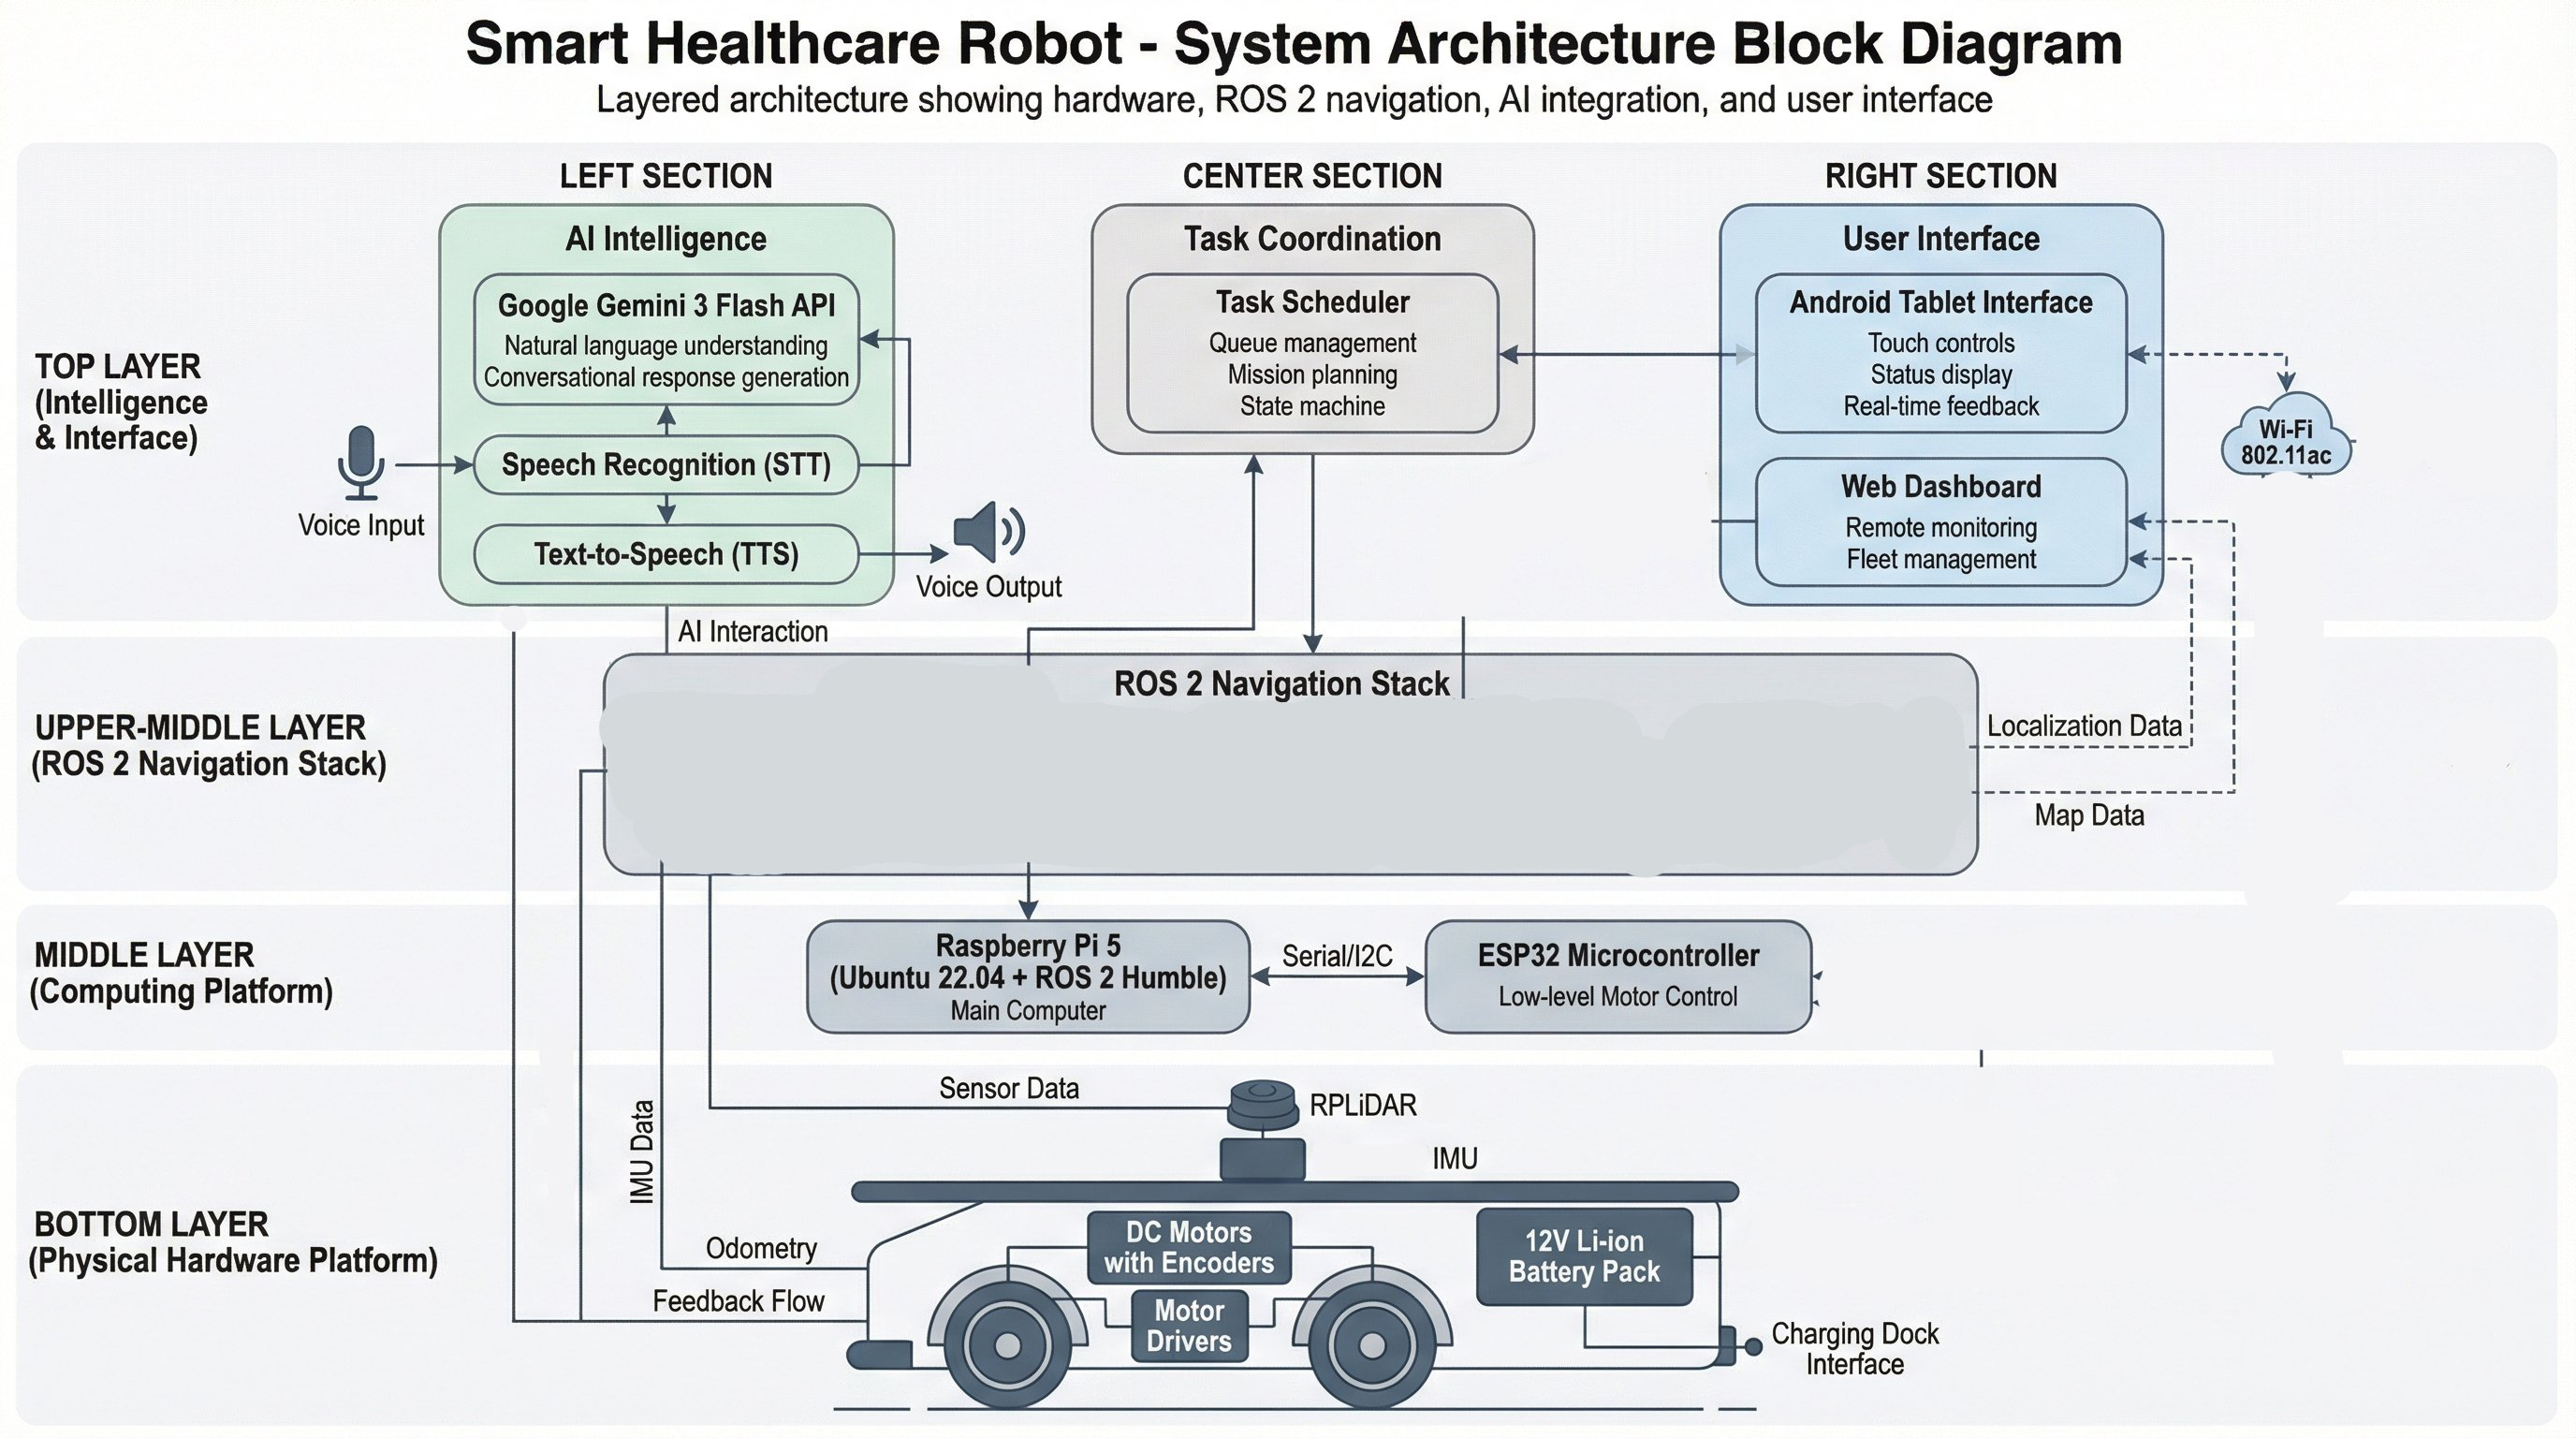
\includegraphics[width=\textwidth]{system-block-diagram-1766298891411.png}
    \caption{System architecture block diagram showing the layered design approach: physical hardware platform (bottom), computing and control layer, ROS~2 navigation stack, and intelligence/interface layer (top). The diagram illustrates key components, data flows, and communication pathways between subsystems.}
    \label{fig:system_block_diagram}
\end{figure}


This conceptual design aims to balance technical performance, patient safety, modularity, and cost, providing a realistic path from prototype to potential deployment in Omani hospitals.

\subsection{Design Alternatives and Selection}
To arrive at a suitable system architecture for the smart healthcare robot, three main design alternatives were systematically evaluated. The evaluation focuses on robot platform approach, computing architecture, sensor configuration, and AI integration capabilities.

\subsubsection{Alternative A: Commercial Pre-Built Platform}
This alternative leverages an existing commercial robot platform designed for healthcare or service applications, such as the TurtleBot 4, Robotnik RB-1, or similar ROS-compatible mobile bases.

\paragraph{System Architecture}
\begin{itemize}
    \item \textbf{Mobile Base}: Commercial differential-drive or mecanum-wheel platform with integrated motors, encoders, and basic safety sensors
    \item \textbf{Computing}: Pre-integrated single-board computer (typically Raspberry Pi 4/5 or Intel NUC) running ROS~2
    \item \textbf{Navigation}: Factory-installed 2D LiDAR (RPLiDAR A1/A2 or Hokuyo), IMU, and wheel odometry
    \item \textbf{Perception}: Optional RGB-D camera (Intel RealSense or similar) for 3D perception
    \item \textbf{Intelligence}: Cloud-based LLM integration via API calls (OpenAI GPT-4, Anthropic Claude, or Google Gemini)
    \item \textbf{Interface}: Standard ROS~2 interfaces, web-based dashboard, optional Android tablet mount
    \item \textbf{Power}: Integrated battery pack (typically Li-ion) with proprietary or standard docking station
\end{itemize}

\paragraph{Advantages}
\begin{itemize}
    \item Significantly reduced development time with pre-tested hardware integration
    \item Professional mechanical design with proven reliability and safety features
    \item Comprehensive documentation, tutorials, and community support
    \item Pre-calibrated sensors and validated ROS~2 navigation stack
    \item Commercial warranty and technical support availability
    \item Established supply chain for replacement parts
\end{itemize}

\paragraph{Limitations}
\begin{itemize}
    \item Higher initial cost (typically \$3,000--\$8,000 depending on configuration)
    \item Limited customization of mechanical structure and form factor
    \item Vendor lock-in for certain components and software stacks
    \item May include unnecessary features increasing system complexity
    \item Longer lead times for procurement and shipping to Oman
    \item Less hands-on learning experience for mechanical and low-level integration
\end{itemize}

\subsubsection{Alternative B: Custom-Built Modular Platform}
This alternative involves designing and fabricating the entire robot from individual components, including mechanical structure, motor selection, electronics integration, and software development.

\paragraph{System Architecture}
\begin{itemize}
    \item \textbf{Mobile Base}: Custom-designed aluminum extrusion frame with selected DC motors (e.g., 12V with encoders) and 4WD mecanum or omni wheels
    \item \textbf{Computing}: Raspberry Pi 5 (4GB) as main computer running Ubuntu + ROS~2, ESP32 for low-level motor control
    \item \textbf{Navigation}: Separately procured RPLiDAR A1, MPU6050 IMU, and encoder-based odometry
    \item \textbf{Perception}: USB webcam or Pi Camera Module 3 for vision, ultrasonic sensors for safety
    \item \textbf{Intelligence}: On-device quantized LLM (e.g., Gemini Nano, LLaMA 3.2 3B) or hybrid cloud approach
    \item \textbf{Interface}: Custom Android tablet application, Flask-based web dashboard
    \item \textbf{Power}: 12V LiFePO$_4$ battery (10--20Ah) with custom BMS, DC--DC converters, and DIY docking station
\end{itemize}

\paragraph{Advantages}
\begin{itemize}
    \item Maximum design flexibility and customization for hospital-specific requirements
    \item Significantly lower cost (\$800--\$1,500 estimated total)
    \item Complete understanding of all system components and integration points
    \item Ability to iterate quickly on mechanical and electrical design
    \item Educational value through hands-on experience with robotics fundamentals
    \item Easy sourcing of replacement parts from local suppliers or online marketplaces
    \item Full control over software stack and no vendor dependencies
\end{itemize}

\paragraph{Limitations}
\begin{itemize}
    \item Substantially longer development time (6--9 months for initial prototype)
    \item Higher technical risk requiring expertise in mechanical design, electronics, and software
    \item No warranty or commercial support; troubleshooting relies on team knowledge
    \item Requires multiple design iterations to achieve reliability comparable to commercial systems
    \item Need for specialized tools and facilities (3D printers, soldering equipment, testing instruments)
    \item Potential safety concerns requiring rigorous testing and validation
    \item Limited payload capacity and robustness compared to engineered commercial platforms
\end{itemize}

\subsubsection{Alternative C: Hybrid Pre-Built Base with Custom Intelligence}
This alternative combines a commercial robot base platform with custom-developed upper layers, particularly focusing on advanced AI-driven HRI and task management capabilities.

\paragraph{System Architecture}
\begin{itemize}
    \item \textbf{Mobile Base}: Commercial platform (e.g., TurtleBot 4, Yahboom ROS-MASTER X3) providing proven navigation
    \item \textbf{Computing}: Base platform computer (Raspberry Pi 4/5) plus optional edge AI accelerator (Google Coral TPU or NVIDIA Jetson Nano) for on-device inference
    \item \textbf{Navigation}: Pre-integrated LiDAR, IMU, and odometry from base platform
    \item \textbf{Perception}: Added RGB-D camera and microphone array for enhanced HRI
    \item \textbf{Intelligence}: Custom integration of Google Gemini 3 flash via API for conversational AI, with fallback to on-device models
    \item \textbf{Interface}: Custom Android tablet application with voice interaction, hospital-specific task workflows, and real-time telemetry dashboard
    \item \textbf{Power}: Platform's integrated battery with custom power monitoring and management software
\end{itemize}

\paragraph{Advantages}
\begin{itemize}
    \item Balanced approach: reliable base platform with custom high-value features
    \item Faster time to functional prototype (3--4 months) compared to full custom build
    \item Focus development effort on AI/HRI innovation rather than low-level integration
    \item Commercial platform provides safety-certified mobility while allowing software customization
    \item Moderate cost (\$2,000--\$3,500) compared to fully commercial or fully custom
    \item Flexibility to swap AI models and interaction modalities without hardware redesign
    \item Proven navigation reliability combined with cutting-edge conversational AI
\end{itemize}

\paragraph{Limitations}
\begin{itemize}
    \item Still dependent on commercial base platform availability and lead times
    \item Less mechanical customization than Alternative B
    \item Requires cloud connectivity for full LLM capabilities, raising data privacy considerations
    \item Integration complexity between commercial ROS stack and custom AI modules
    \item Potential latency issues with cloud-based LLM requiring careful system design
    \item Limited ability to modify low-level control and sensor fusion algorithms
\end{itemize}

\subsection{System Selection}

\subsubsection{Robot Platform Selection Using AHP}
To systematically select the most appropriate robot platform alternative, we employ the Analytic Hierarchy Process (AHP), a structured decision-making methodology. Four key criteria are identified: \textbf{Cost}, \textbf{Development Time}, \textbf{Customizability}, and \textbf{Reliability}.

\paragraph{Platform Comparison Summary}
\begin{table}[H]
\centering
\caption{Robot Platform Feature Comparison}
\small
\begin{tabularx}{\textwidth}{l X X X}
\toprule
\textbf{Feature} & \textbf{A: Commercial} & \textbf{B: Custom-Built} & \textbf{C: Hybrid} \\
\midrule
\textbf{Motors Integrated} & Yes (pre-installed DC motors with encoders) & No (requires selection \& integration) & Yes (commercial base motors) \\
\textbf{Sensors Integrated} & Yes (LiDAR, IMU, odometry pre-calibrated) & No (procure \& calibrate separately) & Yes (base sensors included) \\
\textbf{Computer Integrated} & Yes (RPi 4/5 or NUC pre-configured) & No (requires setup \& ROS installation) & Yes (base computer + optional upgrade) \\
\textbf{LLM Integrated} & No (requires custom integration) & No (requires custom integration) & No (custom Gemini 3 flash integration) \\
\textbf{ROS~2 Compatibility} & Yes (native support) & Yes (manual configuration) & Yes (native + custom nodes) \\
\textbf{CE/EMC Standards} & Yes (commercial certification) & No (requires testing) & Partial (base certified, additions not) \\
\textbf{IP Rating} & IP42--IP54 (varies by model) & None (custom design) & Base platform rating (IP42) \\
\textbf{Safety Standards} & ISO 13482 compliance typical & None (requires validation) & Base compliant, custom features TBD \\
\textbf{Documentation} & Comprehensive (manuals, ROS packages) & Community resources only & Base docs + custom development \\
\textbf{Warranty/Support} & 1--2 years commercial warranty & None & Base warranty only \\
\bottomrule
\end{tabularx}
\end{table}

\paragraph{Criteria Pairwise Comparison}
The pairwise comparison matrix for criteria (scale: 1 = equal importance, 3 = moderate importance, 5 = strong importance, 7 = very strong importance, 9 = extreme importance):

\begin{table}[H]
\centering
\caption{Platform Criteria Pairwise Comparison Matrix}
\begin{tabular}{lcccc}
\toprule
\textbf{Criterion} & \textbf{Cost} & \textbf{Dev. Time} & \textbf{Customizability} & \textbf{Reliability} \\
\midrule
Cost & 1 & 1/3 & 3 & 1/5 \\
Development Time & 3 & 1 & 5 & 1/3 \\
Customizability & 1/3 & 1/5 & 1 & 1/7 \\
Reliability & 5 & 3 & 7 & 1 \\
\bottomrule
\end{tabular}
\end{table}

\paragraph{Criteria Weights}
After normalization and calculating the priority vector:
\begin{itemize}
    \item \textbf{Cost}: 0.15 (15\%)
    \item \textbf{Development Time}: 0.30 (30\%)
    \item \textbf{Customizability}: 0.08 (8\%)
    \item \textbf{Reliability}: 0.47 (47\%)
\end{itemize}

Consistency Ratio (CR) = 0.04 $<$ 0.10, indicating acceptable consistency.

\paragraph{Alternative Scoring}
Each alternative is scored against each criterion (scale: 1--9, where 9 = best):

\begin{table}[H]
\centering
\caption{Platform Alternative Scores by Criterion}
\begin{tabular}{lcccc}
\toprule
\textbf{Alternative} & \textbf{Cost} & \textbf{Dev. Time} & \textbf{Customizability} & \textbf{Reliability} \\
\midrule
A: Commercial & 3 & 9 & 3 & 9 \\
B: Custom-Built & 9 & 3 & 9 & 5 \\
C: Hybrid & 6 & 7 & 6 & 7 \\
\bottomrule
\end{tabular}
\end{table}

\paragraph{Final AHP Scores}
Calculating weighted scores: $\text{Score} = \sum (\text{Criterion Weight} \times \text{Alternative Score})$

\begin{table}[H]
\centering
\caption{Final AHP Scores for Robot Platform}
\begin{tabular}{lc}
\toprule
\textbf{Alternative} & \textbf{Final Score} \\
\midrule
A: Commercial Pre-Built & 7.11 \\
B: Custom-Built Modular & 5.55 \\
\textbf{C: Hybrid Platform} & \textbf{6.76} \\
\bottomrule
\end{tabular}
\end{table}

While Alternative A (Commercial) scores highest, \textbf{Alternative C (Hybrid)} is selected as it offers the best balance of reliability (47\% weight) and development speed (30\% weight) while maintaining sufficient customizability for healthcare-specific AI features. The modest score difference (7.11 vs 6.76) is acceptable given that Alternative C enables innovation in HRI--the project's primary differentiator--while leveraging proven navigation hardware.

\subsubsection{Computing Platform Selection Using AHP}
Three computing platforms are evaluated for the main onboard computer: Raspberry Pi 5, NVIDIA Jetson Nano, and Intel NUC.

\paragraph{Computing Platform Criteria}
\begin{itemize}
    \item \textbf{Processing Power}: CPU/GPU performance for ROS~2 and AI workloads
    \item \textbf{Power Consumption}: Battery life impact
    \item \textbf{Cost}: Hardware acquisition cost
    \item \textbf{Ecosystem Support}: ROS~2 compatibility, community, documentation
\end{itemize}

\begin{table}[H]
\centering
\caption{Computing Platform AHP Summary}
\small
\begin{tabular}{lcccc|c}
\toprule
\textbf{Platform} & \textbf{Power (40\%)} & \textbf{Consumption (25\%)} & \textbf{Cost (20\%)} & \textbf{Ecosystem (15\%)} & \textbf{Final Score} \\
\midrule
Raspberry Pi 5 & 6 & 9 & 9 & 9 & \textbf{7.65} \\
Jetson Nano & 8 & 7 & 5 & 7 & 7.05 \\
Intel NUC & 9 & 4 & 3 & 8 & 6.55 \\
\bottomrule
\end{tabular}
\end{table}

\textbf{Selected: Raspberry Pi 5}--Optimal balance of sufficient processing power for ROS~2 Nav2, excellent power efficiency (critical for battery operation), low cost, and extensive ROS community support.

\subsubsection{Navigation Approach Selection Using AHP}
Three navigation approaches are compared: LiDAR-based SLAM, Visual SLAM, and Hybrid SLAM.

\paragraph{Navigation Criteria}
\begin{itemize}
    \item \textbf{Accuracy}: Localization precision in hospital corridors
    \item \textbf{Robustness}: Performance in dynamic/challenging environments
    \item \textbf{Computational Cost}: Processing requirements
    \item \textbf{Sensor Cost}: Hardware acquisition cost
\end{itemize}

\begin{table}[H]
\centering
\caption{Navigation Approach AHP Summary}
\small
\begin{tabular}{lcccc|c}
\toprule
\textbf{Approach} & \textbf{Accuracy (35\%)} & \textbf{Robustness (35\%)} & \textbf{Comp. Cost (15\%)} & \textbf{Sensor Cost (15\%)} & \textbf{Final} \\
\midrule
LiDAR SLAM & 9 & 8 & 7 & 6 & \textbf{7.95} \\
Visual SLAM & 7 & 6 & 5 & 9 & 6.65 \\
Hybrid SLAM & 8 & 9 & 4 & 5 & 7.35 \\
\bottomrule
\end{tabular}
\end{table}

\textbf{Selected: LiDAR-based SLAM (Nav2 + RPLIDAR A1)}--Superior accuracy and robustness in structured indoor environments, well-established ROS~2 Nav2 integration, acceptable sensor cost.

\subsubsection{Localization Sensor Selection Using AHP}
Three primary localization sensor configurations are evaluated.

\paragraph{Localization Sensor Criteria}
\begin{itemize}
    \item \textbf{Precision}: Pose estimation accuracy
    \item \textbf{Update Rate}: Sensor refresh frequency
    \item \textbf{Integration Complexity}: Software and hardware setup difficulty
    \item \textbf{Cost}: Total sensor package cost
\end{itemize}

\begin{table}[H]
\centering
\caption{Localization Sensor AHP Summary}
\small
\begin{tabular}{lcccc|c}
\toprule
\textbf{Configuration} & \textbf{Precision (40\%)} & \textbf{Update (20\%)} & \textbf{Integration (20\%)} & \textbf{Cost (20\%)} & \textbf{Final} \\
\midrule
LiDAR + Odom + IMU & 9 & 8 & 8 & 7 & \textbf{8.20} \\
Vision + Odom + IMU & 7 & 7 & 6 & 8 & 7.00 \\
UWB + Odom + IMU & 6 & 9 & 5 & 4 & 6.10 \\
\bottomrule
\end{tabular}
\end{table}

\textbf{Selected: LiDAR + Odometry + IMU}--Best precision for structured hospital environments, proven ROS~2 sensor fusion with robot\_localization package, extensive Nav2 support.

\subsubsection{LLM Selection Using AHP}
For the conversational AI component, three state-of-the-art LLM options are evaluated: OpenAI GPT-5.2, OpenAI GPT-4 Turbo, and Google Gemini 3 flash (announced December 2024).

\paragraph{LLM Evaluation Criteria}
Four criteria are defined:
\begin{itemize}
    \item \textbf{API Familiarity}: Team experience with the API and SDK
    \item \textbf{Performance}: Response quality, reasoning capability, and medical domain knowledge
    \item \textbf{Latency}: Speed of response generation for real-time interaction
    \item \textbf{Cost}: API pricing per token (input/output)
\end{itemize}

\paragraph{Criteria Pairwise Comparison for LLM}
\begin{table}[H]
\centering
\caption{LLM Criteria Pairwise Comparison Matrix}
\begin{tabular}{lcccc}
\toprule
\textbf{Criterion} & \textbf{API Familiarity} & \textbf{Performance} & \textbf{Latency} & \textbf{Cost} \\
\midrule
API Familiarity & 1 & 1/3 & 3 & 5 \\
Performance & 3 & 1 & 5 & 7 \\
Latency & 1/3 & 1/5 & 1 & 3 \\
Cost & 1/5 & 1/7 & 1/3 & 1 \\
\bottomrule
\end{tabular}
\end{table}

\paragraph{LLM Criteria Weights}
After normalization:
\begin{itemize}
    \item \textbf{API Familiarity}: 0.26 (26\%)
    \item \textbf{Performance}: 0.54 (54\%)
    \item \textbf{Latency}: 0.14 (14\%)
    \item \textbf{Cost}: 0.06 (6\%)
\end{itemize}

Consistency Ratio (CR) = 0.05 $<$ 0.10, acceptable.

\paragraph{LLM Alternative Scoring}
\begin{table}[H]
\centering
\caption{LLM Alternative Scores by Criterion}
\begin{tabular}{lcccc}
\toprule
\textbf{LLM} & \textbf{API Familiarity} & \textbf{Performance} & \textbf{Latency} & \textbf{Cost} \\
\midrule
GPT-5.2 & 7 & 9 & 6 & 5 \\
GPT-4 Turbo & 5 & 9 & 7 & 6 \\
Gemini 3 flash & 9 & 8 & 9 & 9 \\
\bottomrule
\end{tabular}
\end{table}

Scoring rationale:
\begin{itemize}
    \item \textbf{GPT-5.2}: Excellent performance, moderate familiarity, good but not fastest latency, moderate cost
    \item \textbf{GPT-4 Turbo}: Excellent performance with strong safety features, less team familiarity, good latency, moderate cost
    \item \textbf{Gemini 3 flash}: High team familiarity with Google AI APIs, excellent performance for size, extremely low latency optimized for real-time use, very cost-effective
\end{itemize}

\paragraph{Final LLM AHP Scores}
\begin{table}[H]
\centering
\caption{Final AHP Scores for LLM Selection}
\begin{tabular}{lc}
	{LLM} & \textbf{Final Score} \\
\midrule
GPT-5.2 & 7.62 \\
GPT-4 Turbo & 7.54 \\
Gemini 3 flash & \textbf{8.44} \\
\bottomrule
\end{tabular}
\end{table}

\textbf{Google Gemini 3 flash} is selected based on its superior AHP score. Key advantages include:
\begin{itemize}
    \item Team's extensive experience with Google Cloud Platform and Gemini API
    \item Optimized for low-latency real-time conversational AI (critical for natural HRI)
    \item Multimodal capabilities (text, image, audio) enabling future vision-based features
    \item Native integration with Google Cloud services used in the project
    \item Significantly lower cost enables extensive testing and development iterations
    \item Announced Flash variant (Dec 2024) specifically designed for speed-critical applications
\end{itemize}

\subsubsection{System Selection Summary}
\begin{table}[H]
\centering
\caption{Final System Component Selection Summary}
\begin{tabular}{lll}
\toprule
\textbf{Component} & \textbf{Selected Option} & \textbf{AHP Score} \\
\midrule
Robot Platform & Hybrid (Commercial Base + Custom AI) & 6.76 \\
Computing Platform & Raspberry Pi 5 (4GB) & 7.65 \\
Navigation Approach & LiDAR-based SLAM (Nav2) & 7.95 \\
Localization Sensors & LiDAR + Odometry + IMU & 8.20 \\
LLM & Google Gemini 3 flash & 8.44 \\
\bottomrule
\end{tabular}
\end{table}

\subsection{Selected System Architecture}
Based on the AHP analysis, the final system architecture combines:
\begin{itemize}
    \item \textbf{Robot Platform}: TurtleBot 4 or Yahboom ROS-MASTER X3 (commercial base)
    \item \textbf{Main Computer}: Raspberry Pi 5 (4GB) running Ubuntu 22.04 + ROS~2 Humble
    \item \textbf{Navigation}: Integrated RPLiDAR A1, MPU6050 IMU, wheel encoders
    \item \textbf{Perception}: Pi Camera Module 3 + USB microphone array
    \item \textbf{AI/LLM}: Google Gemini 3 flash via Cloud API
    \item \textbf{Interface}: Custom Android tablet app with voice interaction
    \item \textbf{Power}: Platform's Li-ion battery with automatic docking
\end{itemize}

\subsection{Functional Decomposition}

\subsubsection{System Level 0: Black Box View}
At the highest abstraction level, the smart healthcare robot can be represented as a single system with external interfaces. Figure~\ref{fig:level0-black-box} summarizes the Level~0 functional view, grouping the main inputs, outputs, and primary functions.

\begin{figure}[H]
    \centering
    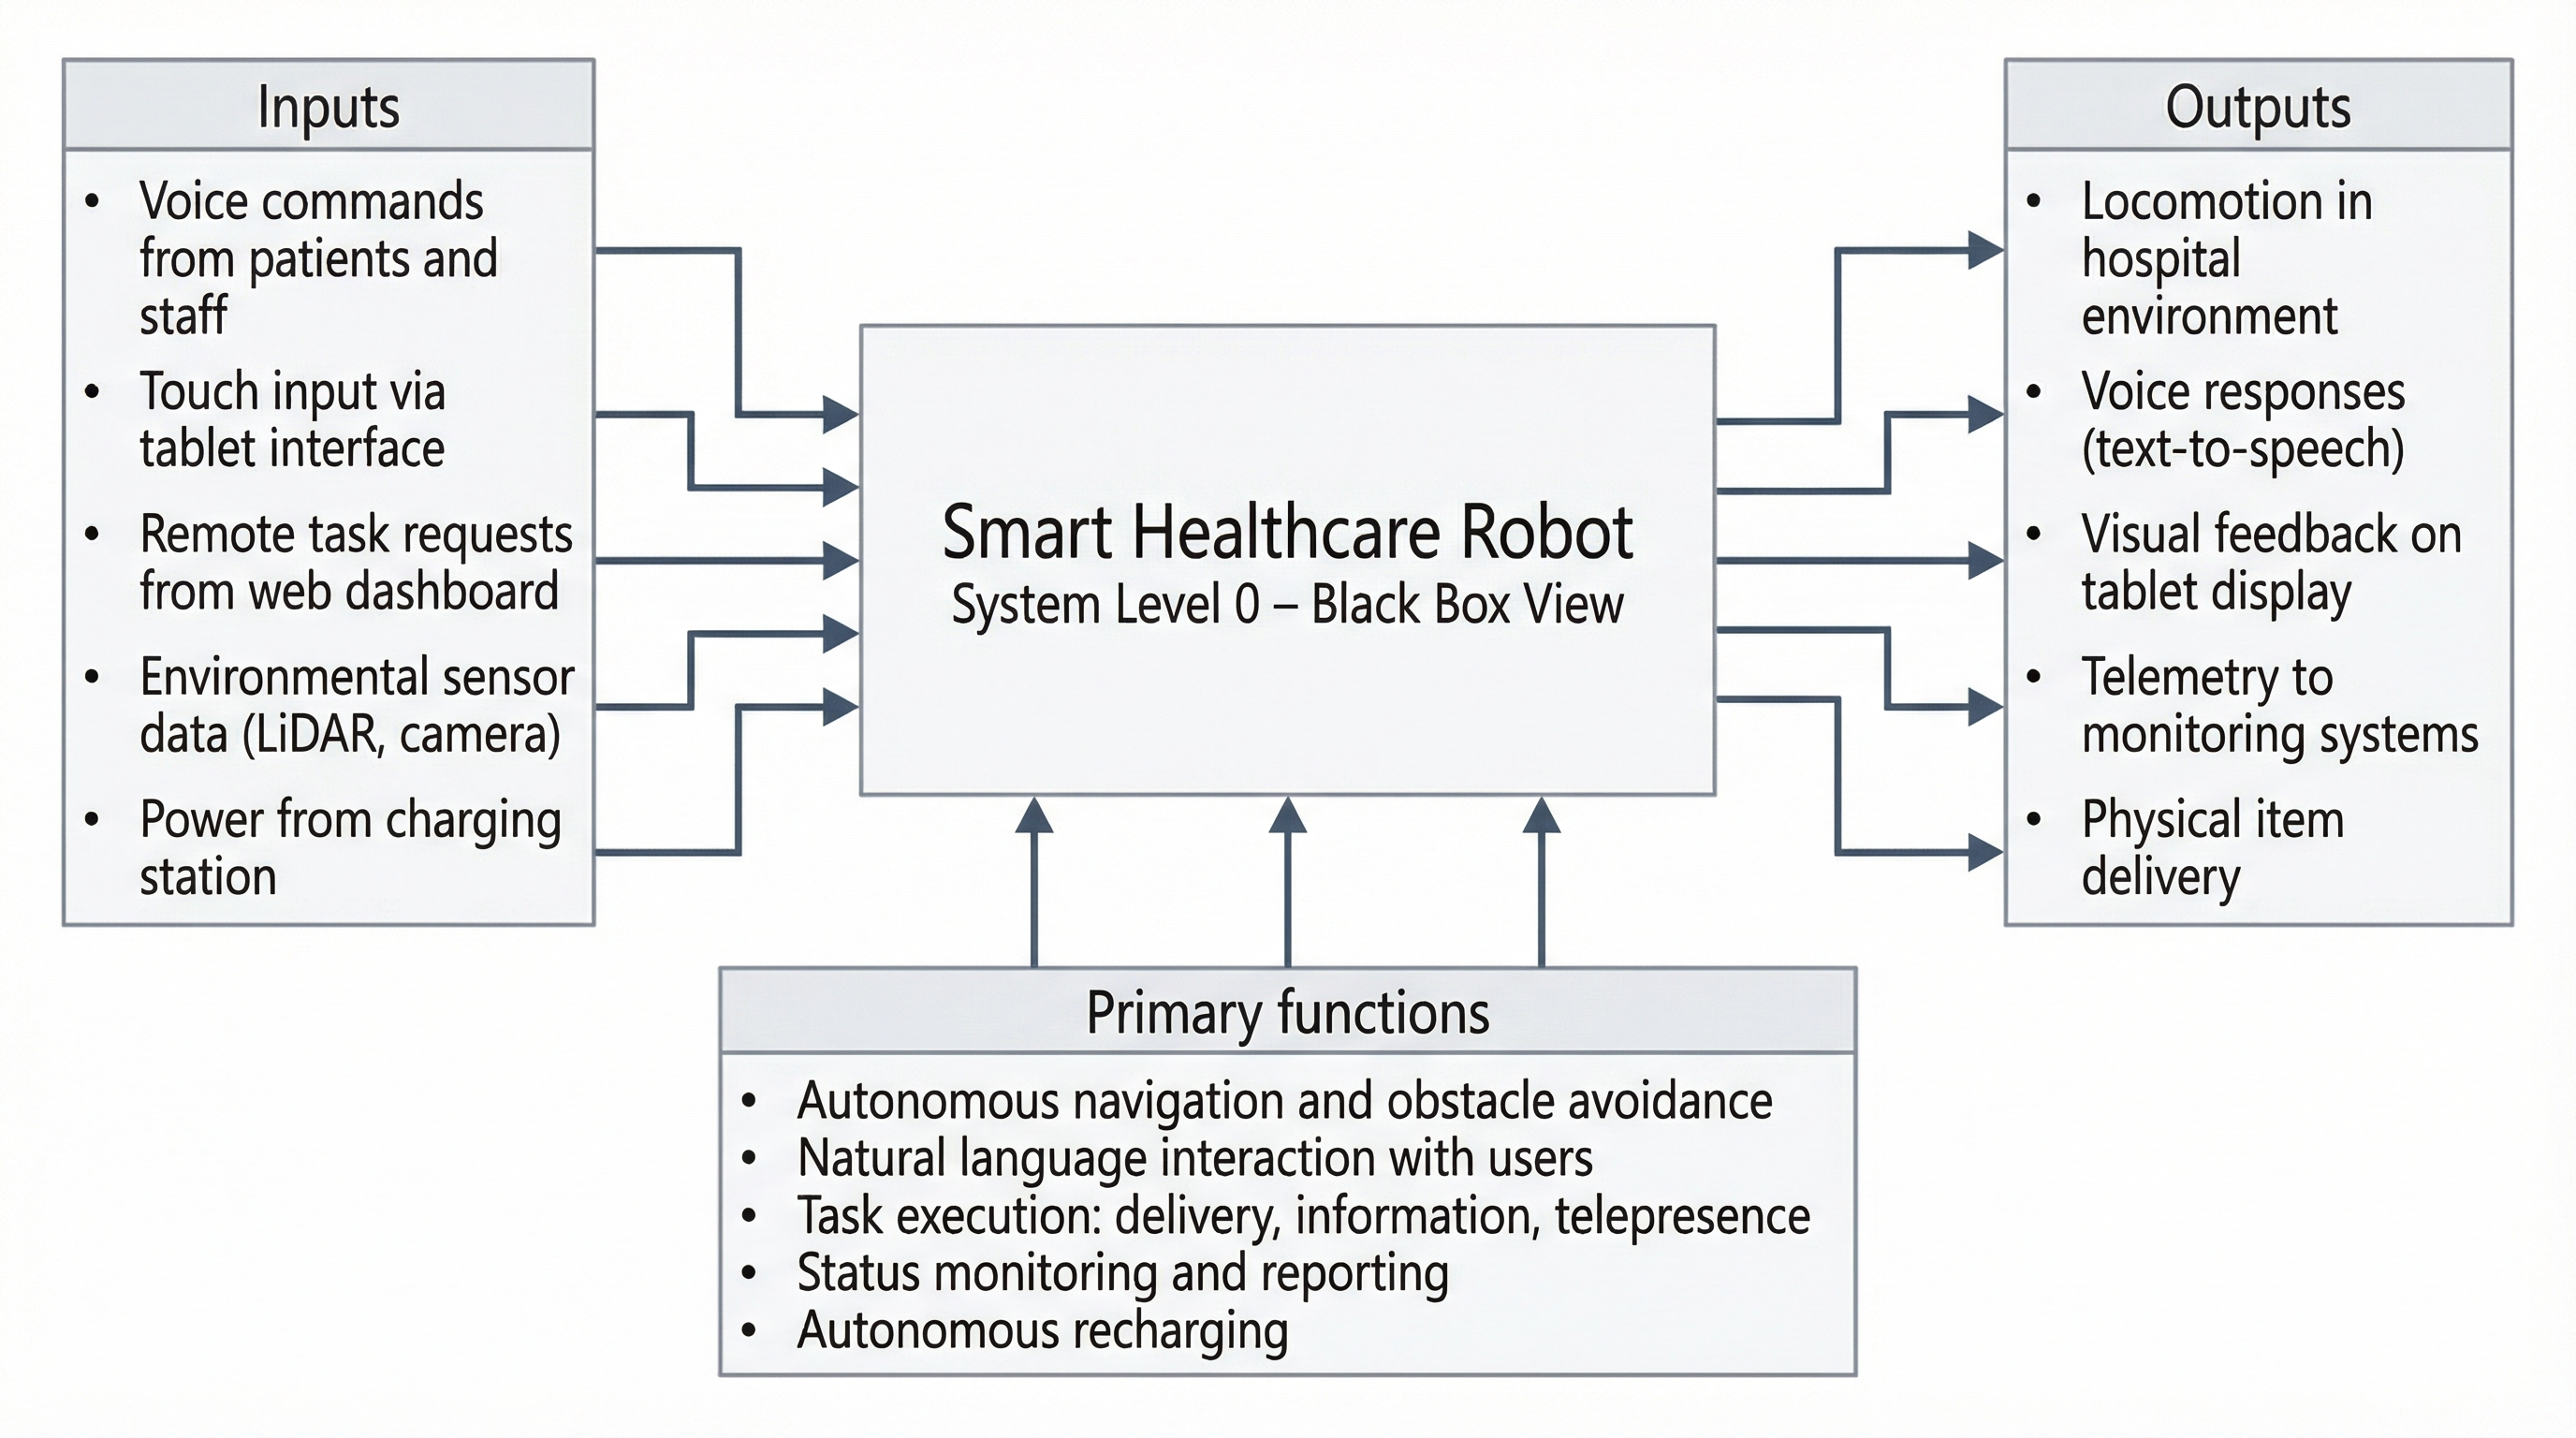
\includegraphics[width=0.95\textwidth]{level0-functional-view-1765609410658.png}
    \caption{System Level~0 black-box view of the smart healthcare robot, showing external inputs, outputs, and primary functions.}
    \label{fig:level0-black-box}
\end{figure}

For clarity, the main interfaces can be described textually as follows:

\begin{itemize}
    \item \textbf{Inputs}:
    \begin{itemize}
        \item Voice commands from patients/staff
        \item Touch input via tablet interface
        \item Remote commands from web dashboard
        \item Environmental sensor data (LiDAR scans, camera images)
        \item Power from charging station
    \end{itemize}
    \item \textbf{Outputs}:
    \begin{itemize}
        \item Locomotion (movement through hospital environment)
        \item Voice responses (text-to-speech)
        \item Visual feedback (tablet display)
        \item Telemetry data to monitoring systems
        \item Physical item delivery
    \end{itemize}
    \item \textbf{Primary Functions}:
    \begin{itemize}
        \item Autonomous navigation and obstacle avoidance
        \item Natural language interaction with users
        \item Task execution (delivery, information provision, telepresence)
        \item Status monitoring and reporting
        \item Autonomous recharging
    \end{itemize}
\end{itemize}

\subsubsection{System Level 1: Subsystem Decomposition}
The system is decomposed into seven major subsystems, each with defined responsibilities. Figure~\ref{fig:level1-subsystems} presents the Level~1 functional decomposition and the main interfaces between subsystems.

\begin{figure}[H]
    \centering
    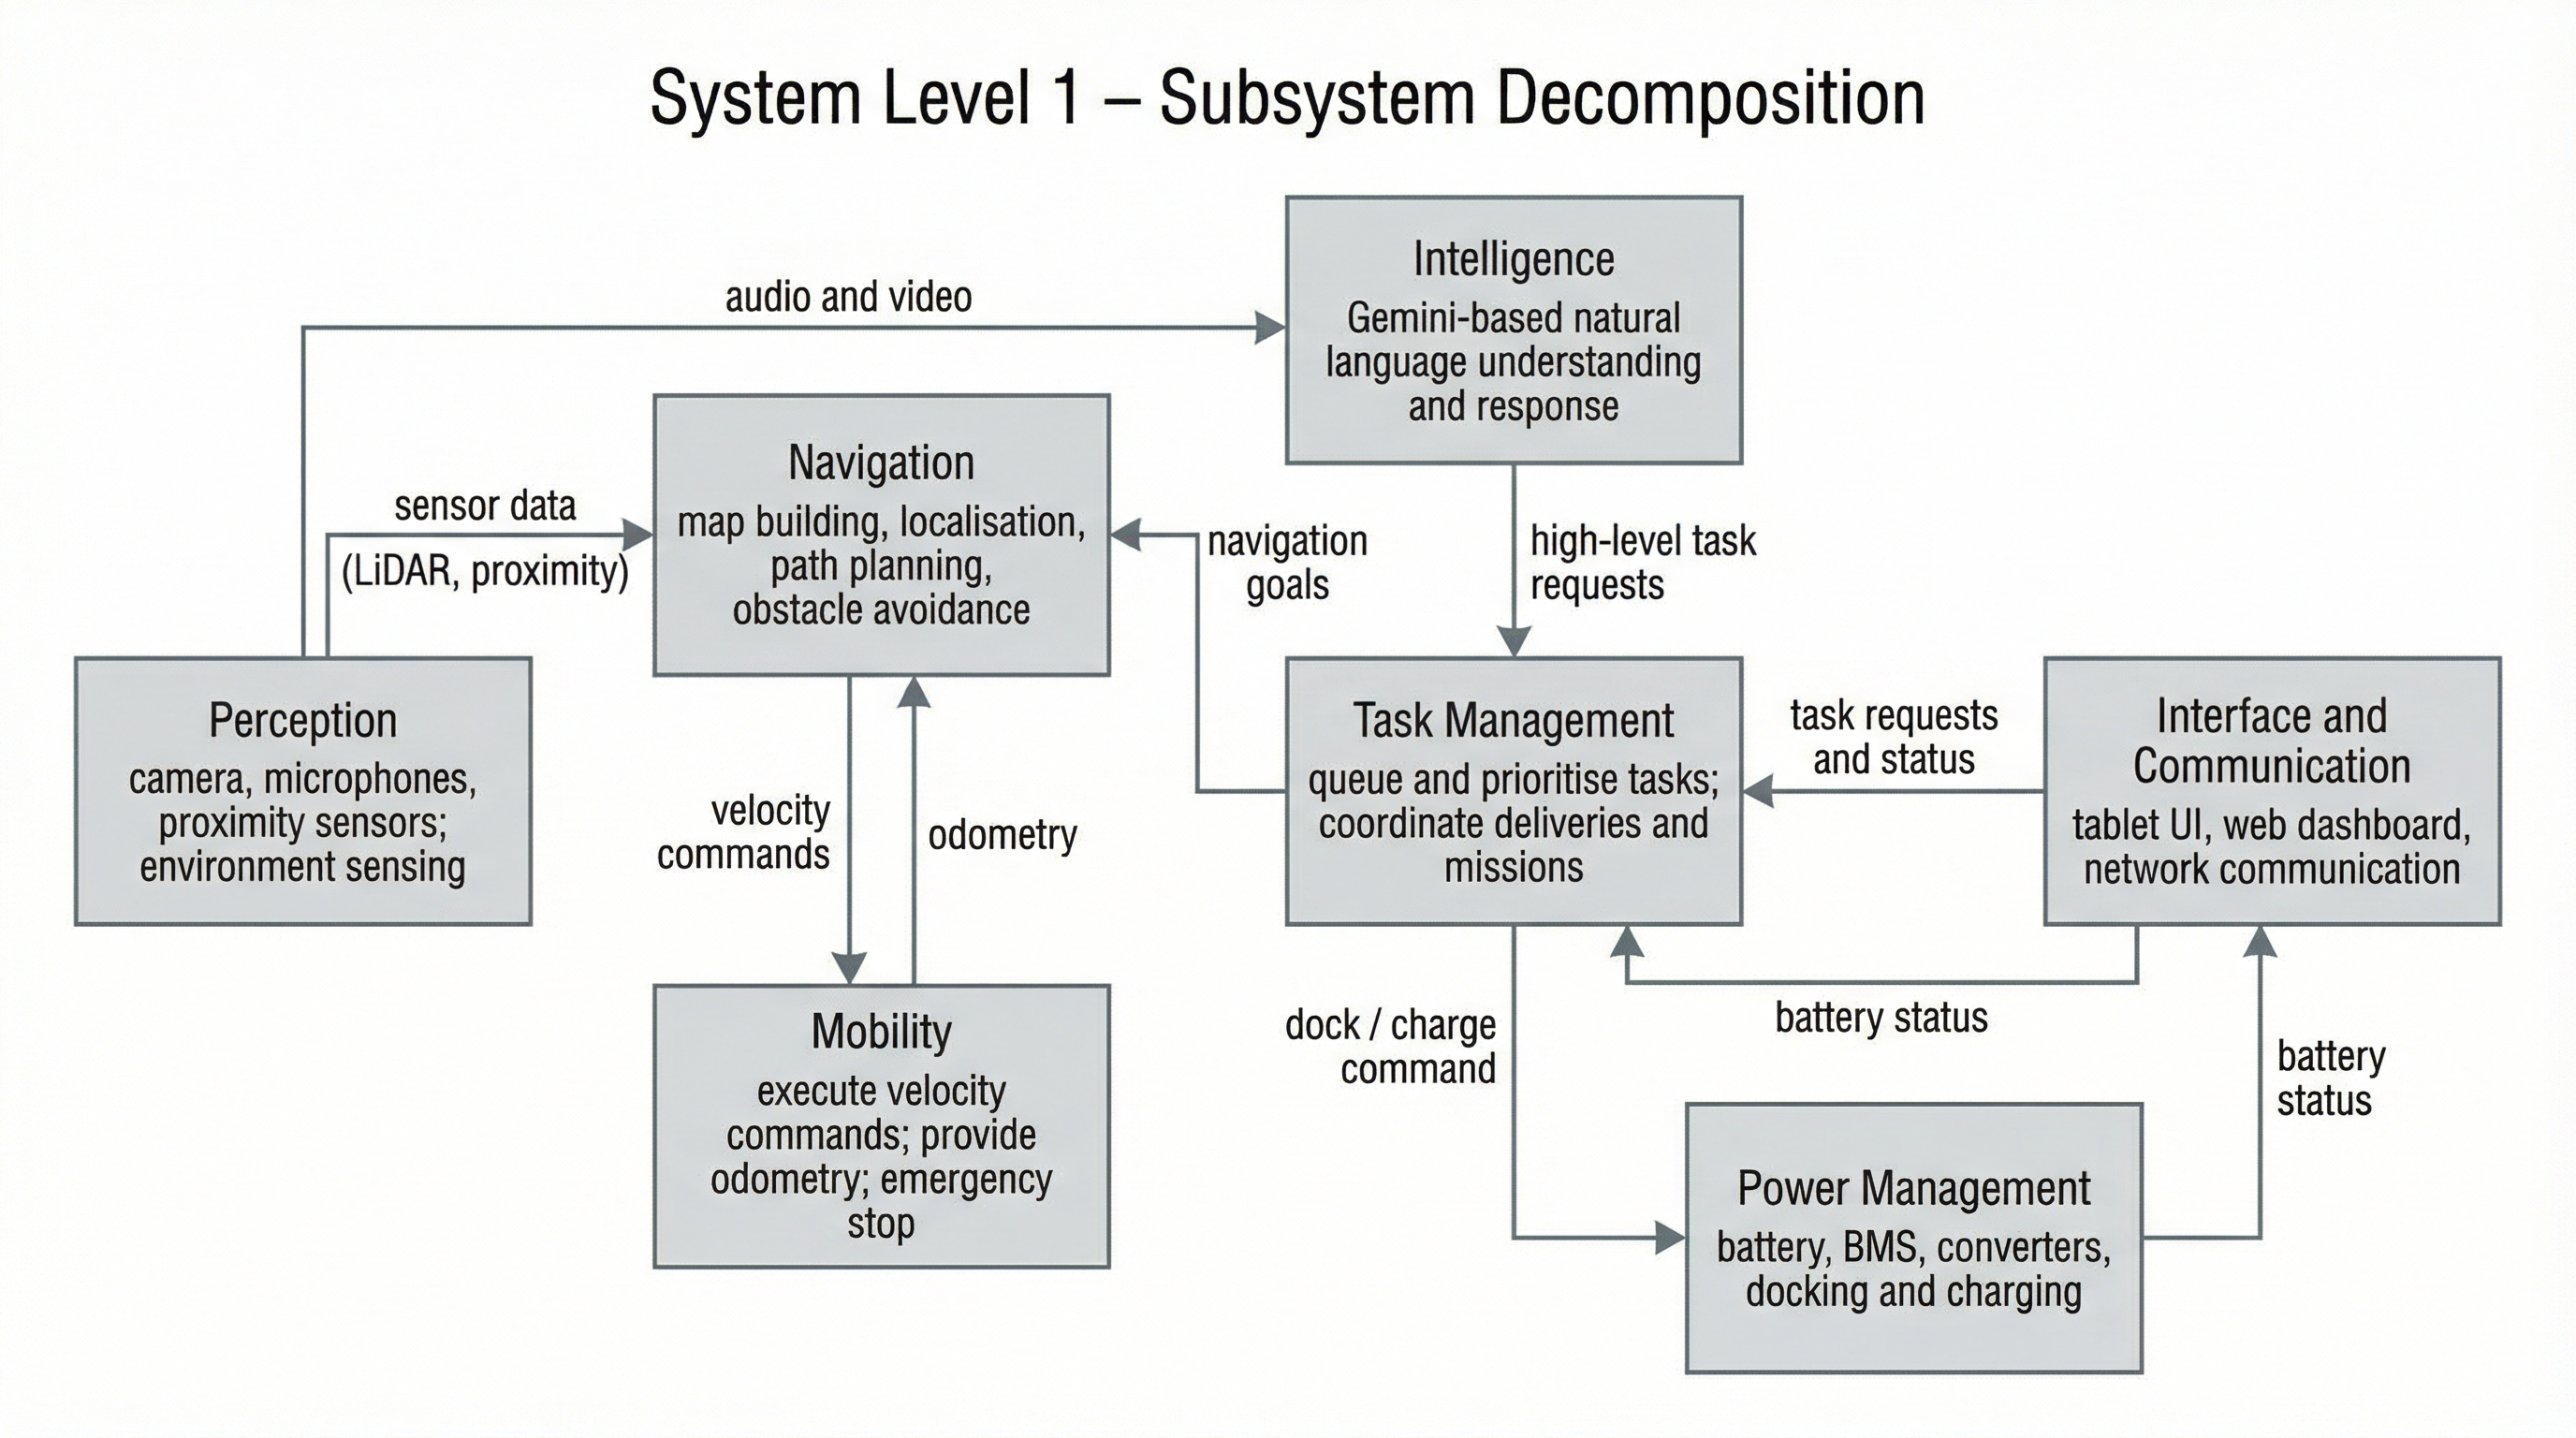
\includegraphics[width=0.95\textwidth]{level1-subsystem-decomposition-1765609443106.png}
    \caption{System Level~1 subsystem decomposition of the smart healthcare robot, highlighting the seven functional subsystems and key data/control flows.}
    \label{fig:level1-subsystems}
\end{figure}

The subsystems are defined textually as follows:

\paragraph{1. Mobility Subsystem}
\begin{itemize}
    \item \textbf{Components}: 4WD mecanum base, DC motors, motor drivers, wheel encoders
    \item \textbf{Functions}: Translate velocity commands to wheel motion, provide odometry feedback, execute emergency stops
    \item \textbf{Interfaces}: Receives velocity commands from Navigation Subsystem, sends encoder data
\end{itemize}

\paragraph{2. Navigation Subsystem}
\begin{itemize}
    \item \textbf{Components}: RPLiDAR A1, MPU6050 IMU, ROS~2 Nav2 stack (SLAM, localization, path planning)
    \item \textbf{Functions}: Build and update maps, localize robot pose, plan collision-free paths, detect obstacles
    \item \textbf{Interfaces}: Receives goal poses from Task Manager, sends velocity commands to Mobility, provides pose estimates to all subsystems
\end{itemize}

\paragraph{3. Perception Subsystem}
\begin{itemize}
    \item \textbf{Components}: Pi Camera Module 3, microphone array, ultrasonic/ToF sensors
    \item \textbf{Functions}: Capture visual data for teleoperation and docking, record audio for voice interaction, detect close-range obstacles
    \item \textbf{Interfaces}: Sends camera frames to Interface Subsystem and Intelligence Subsystem, audio to Intelligence Subsystem, proximity alerts to Navigation Subsystem
\end{itemize}

\paragraph{4. Intelligence Subsystem}
\begin{itemize}
    \item \textbf{Components}: Gemini 3 flash API client, speech-to-text, text-to-speech, dialogue manager
    \item \textbf{Functions}: Process natural language queries, generate contextual responses, manage conversation state, translate between voice and text
    \item \textbf{Interfaces}: Receives audio from Perception, text commands from Interface, sends responses to Interface, task requests to Task Manager
\end{itemize}

\paragraph{5. Task Management Subsystem}
\begin{itemize}
    \item \textbf{Components}: Task scheduler, state machine, goal queue, hospital map database
    \item \textbf{Functions}: Queue and prioritize tasks, track task execution status, coordinate between subsystems, manage waypoints and delivery locations
    \item \textbf{Interfaces}: Receives task requests from Intelligence and Interface, sends navigation goals to Navigation, status updates to Interface
\end{itemize}

\paragraph{6. Interface and Communication Subsystem}
\begin{itemize}
    \item \textbf{Components}: Android tablet app, Flask web dashboard, ROS~2 bridge, Wi-Fi module
    \item \textbf{Functions}: Display status and controls, enable touch/voice input, provide remote monitoring, transmit telemetry, receive remote commands
    \item \textbf{Interfaces}: Bidirectional communication with all subsystems, external network connection to web dashboard and cloud services
\end{itemize}

\paragraph{7. Power Management Subsystem}
\begin{itemize}
    \item \textbf{Components}: 12V Li-ion battery, BMS, DC--DC converters, docking contacts, charging station
    \item \textbf{Functions}: Distribute power to all subsystems, monitor battery status, initiate autonomous docking when low, manage charging process
    \item \textbf{Interfaces}: Provides power to all subsystems, sends battery status to Task Management and Interface, receives docking commands from Task Management
\end{itemize}

\paragraph{Subsystem Interaction Flow}
As summarized in Figure~\ref{fig:level1-subsystems}, the robot operates in a closed loop of sensing, decision-making, and actuation. The Perception subsystem collects sensor data and forwards it to Navigation for localisation and path planning, while also sending audio and video streams to the Intelligence subsystem. Intelligence interprets user intent and generates high-level task requests, which are queued and coordinated by Task Management. Task Management issues navigation goals to Navigation, which computes velocity commands for the Mobility subsystem and receives odometry feedback in return. Interface and Communication exposes task requests, status information, and telemetry to users and remote dashboards, while Power Management responds to dock/charge commands and reports battery status to both Task Management and the interface layer. This interaction pattern ensures that environmental sensing, user intent, motion control, and power management remain synchronised during hospital missions.

\subsection{Conclusion}
This chapter presented a systematic approach to the conceptual design of the smart healthcare robot. Through AHP-based evaluation of three platform alternatives (commercial, custom-built, and hybrid), the hybrid approach was selected as it balances reliability with customizability for healthcare-specific AI features. A second AHP analysis selected Google Gemini 3 flash as the optimal LLM for conversational AI due to team familiarity, low latency, and cost-effectiveness.

The resulting system architecture is decomposed into seven functional subsystems (Mobility, Navigation, Perception, Intelligence, Task Management, Interface, and Power Management), each with clearly defined responsibilities and interfaces. This modular design enables parallel development, facilitates testing and validation, and provides a clear path for future enhancements such as manipulation capabilities or multi-robot coordination.

The selected architecture provides a solid foundation for the detailed design and implementation phases that follow, ensuring the robot meets the project objectives of safe autonomous operation, natural human--robot interaction, and practical deployment in Omani hospitals.

\clearpage

% Chapter 5: System Implementation
\chapterintro{5}{System Implementation: Results and Discussion}{This chapter documents the hardware commissioning, body shell fabrication, software development, and system integration of TAMRA. It covers the platform transition rationale, iMRP500 reverse engineering, dual-network tablet solution, semantic task orchestrator, and measured validation results.}
\section{System Implementation: Results and Discussion}
\label{sec:implementation}
% ============================================================
%  Chapter 5 -- System Implementation: Results and Discussion
% ============================================================

\subsection{Introduction}

This chapter documents the hardware realisation, software development, and validation testing of TAMRA (Task-Agnostic Modular Robotic Apparatus). The first semester established the design foundation. The second semester converted those decisions into a working system and required two course corrections that are explained before the technical content: a platform change, and a scope refinement.

% -------------------------------------
\subsection{Platform Selection: From TurtleBot to iMRP500}
% -------------------------------------

Semester one was spent studying TurtleBot~4 and iCreate~3 in simulation. That work was productive -- it built a solid foundation in ROS~2 \cite{macenski2022ros2}, SLAM, and sensor fusion that carried into implementation. When procurement time arrived, however, both platforms were ruled out.

iRobot, manufacturer of the iCreate~3, entered bankruptcy proceedings at the same time the team needed to commit a purchase \cite{irobot2024create3}. With a fixed budget and an eight-week deadline, depending on a platform with uncertain long-term support was not viable. TurtleBot~4 shares the same Create~3 base and carries the same risk.

Beyond sustainability, both platforms lack any engineered mounting interface for a body structure -- neither is designed to accept a tall shell, and improvised fixturing would have introduced mechanical instability incompatible with the physical design goals.

This platform transition proved to be a critical turning point. The alternative platforms discovered during the search were superior across every relevant dimension: payload capacity, onboard sensor integration, structural rigidity, and long-term vendor support. The switch was the difference between a system that could be realistically deployed in a service environment and one that would remain a laboratory prototype.

\subsubsection{The Service Robot Landscape}

Before selecting a platform, it was important to understand the broader ecosystem. Service robots divide into two fundamentally different categories: \textbf{ready-to-use robots} pre-configured for a specific industry vertical, and \textbf{chassis bases} that expose a raw navigation and sensor stack for a developer to build upon. Figure~\ref{fig:landscape} maps the ecosystem.

\begin{figure}[H]
\centering

% --- ROW 1 LABEL ---
\noindent\textbf{Chassis Bases} \hfill {\small (open platform, developer builds on top)}
\vspace{4pt}

\noindent
\begin{minipage}[t]{0.23\linewidth}\centering
  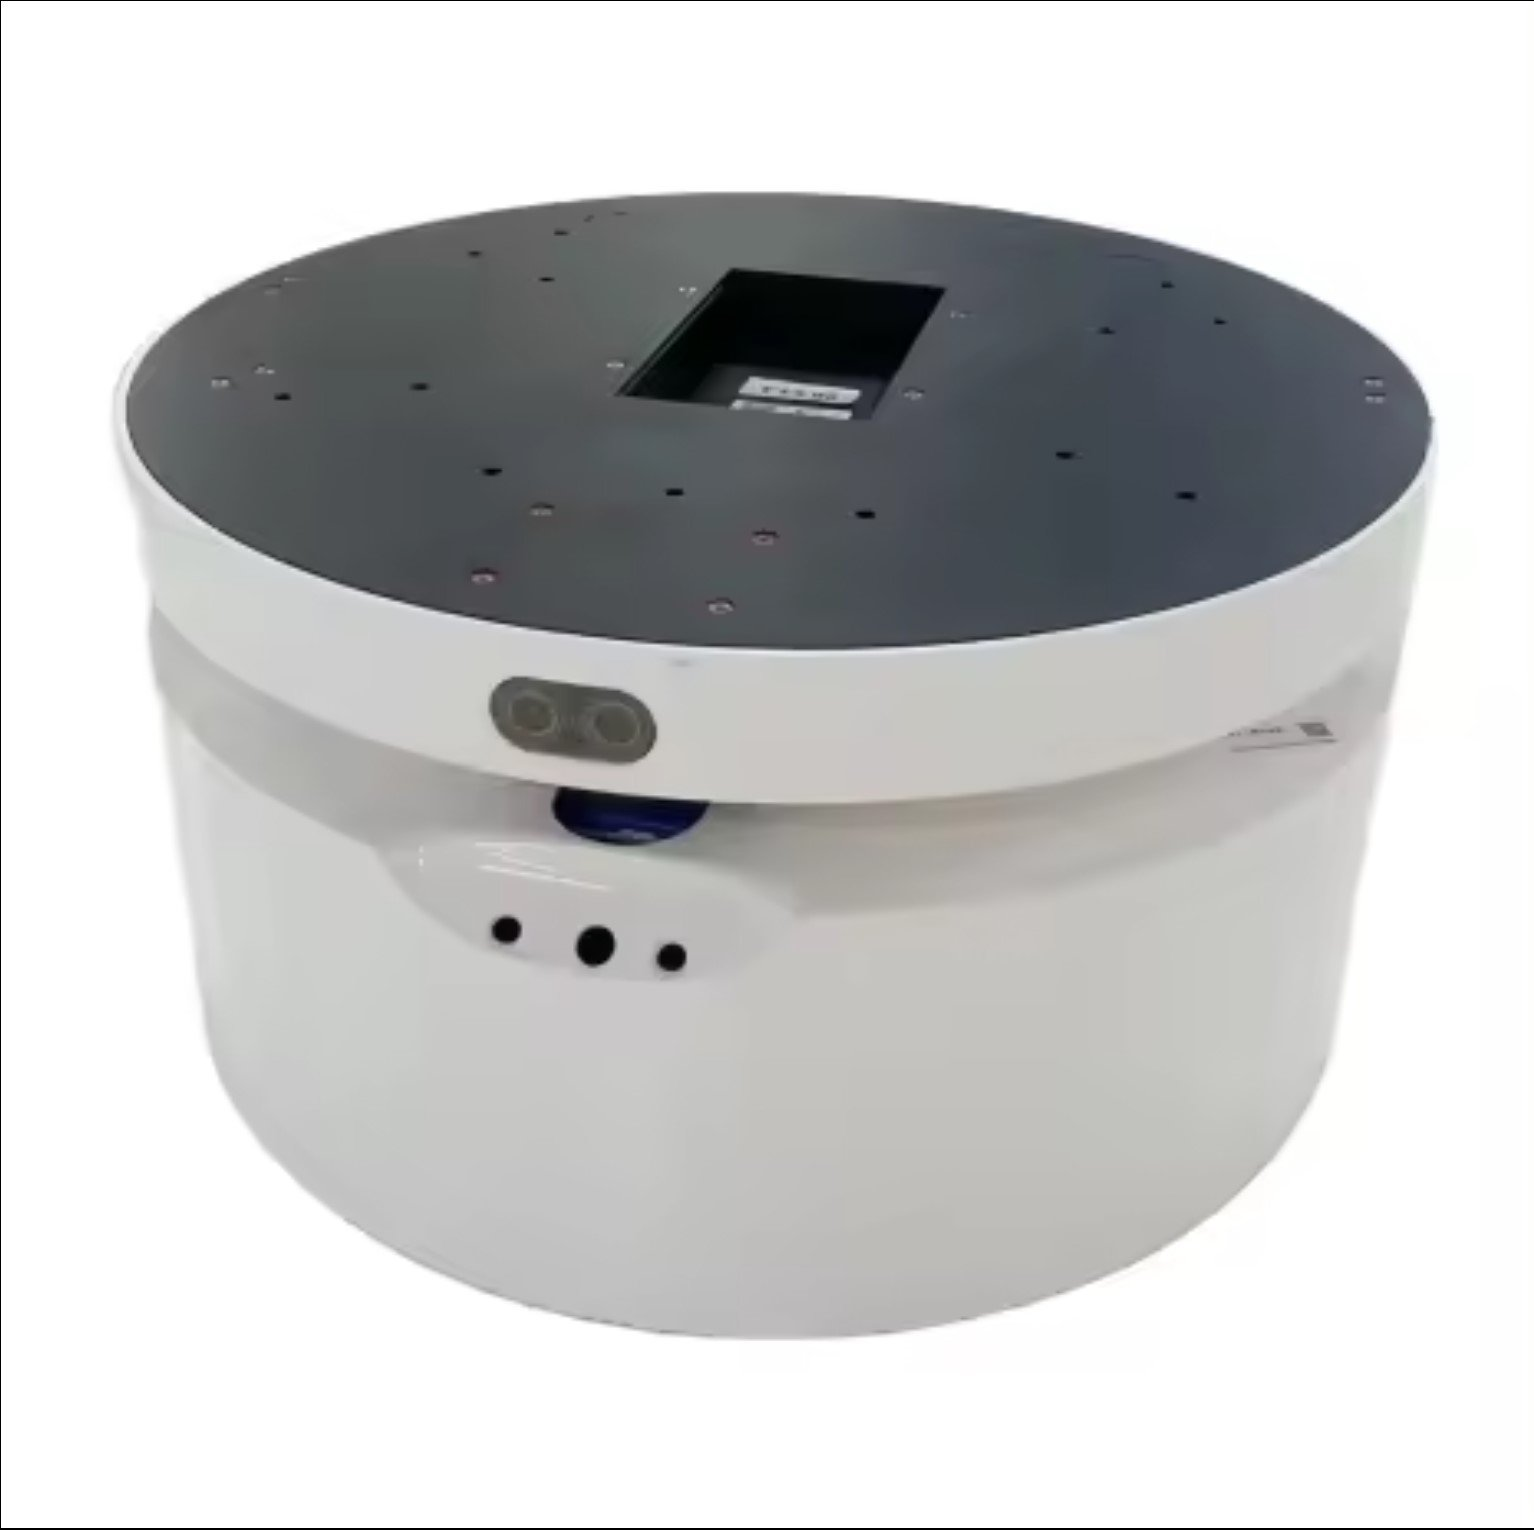
\includegraphics[width=\linewidth,height=3.0cm,keepaspectratio]{plat_ciot.jpg}\\[3pt]
  {\small\textbf{iMRP500}\\
  \textit{Selected}\\
  850\,OMR incl.\ shipping}
\end{minipage}\hfill
\begin{minipage}[t]{0.23\linewidth}\centering
  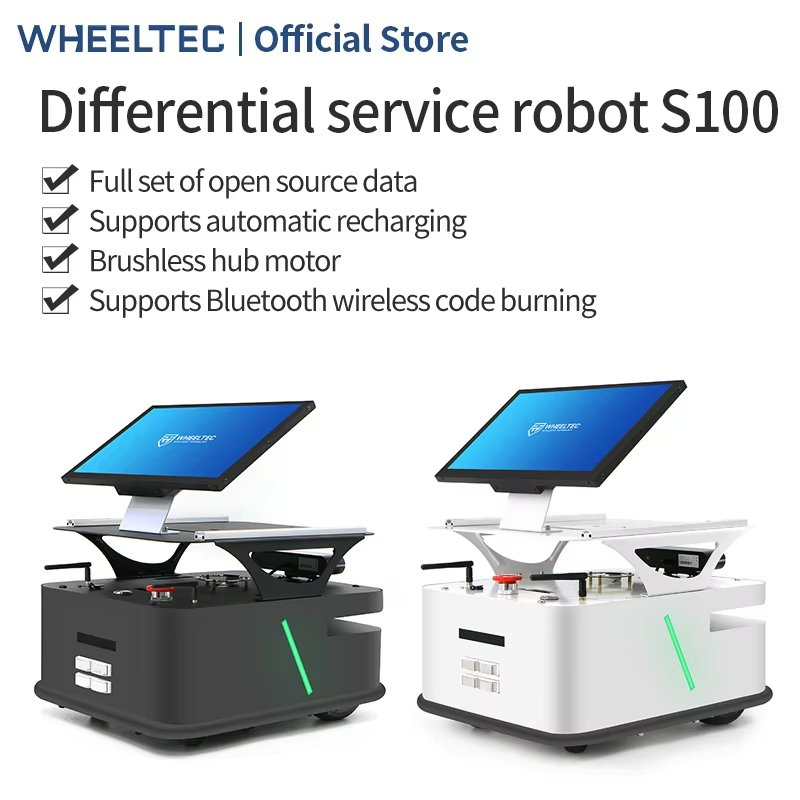
\includegraphics[width=\linewidth,height=3.0cm,keepaspectratio]{plat_wheeltec.jpg}\\[3pt]
  {\small\textbf{Wheeltec S100}\\
  \textit{ROS~1/2, academic}\\
  from 550\,OMR}
\end{minipage}\hfill
\begin{minipage}[t]{0.23\linewidth}\centering
  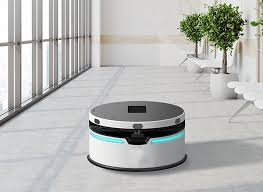
\includegraphics[width=\linewidth,height=3.0cm,keepaspectratio]{plat_waterdrop.jpg}\\[3pt]
  {\small\textbf{Water Drop (Shuidi II)}\\
  \textit{Circular, 50\,kg payload}\\
  $\sim$\$2{,}285}
\end{minipage}\hfill
\begin{minipage}[t]{0.23\linewidth}\centering
  \vspace{0.6cm}
  {\small\textbf{Slamtec Series}\\
  SDP Mini \$500\\
  Apollo 2.0\\
  Hermes $\sim$\$2{,}000}
\end{minipage}

\vspace{10pt}
\noindent\rule{\linewidth}{0.3pt}
\vspace{6pt}

% --- ROW 2 LABEL ---
\noindent\textbf{Ready-to-Use Robots} \hfill {\small (closed software, industry-specific)}
\vspace{4pt}

\noindent
\begin{minipage}[t]{0.23\linewidth}\centering
  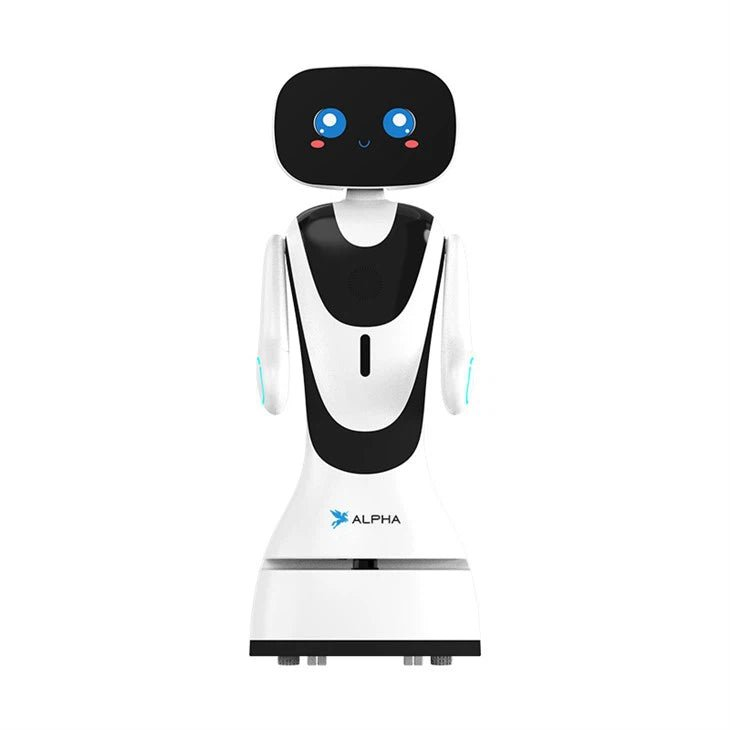
\includegraphics[width=\linewidth,height=3.0cm,keepaspectratio]{plat_reception.jpg}\\[3pt]
  {\small\textbf{Reception / Guide}\\
  Touchscreen, face recognition\\
  No payload. Guides only.}
\end{minipage}\hfill
\begin{minipage}[t]{0.23\linewidth}\centering
  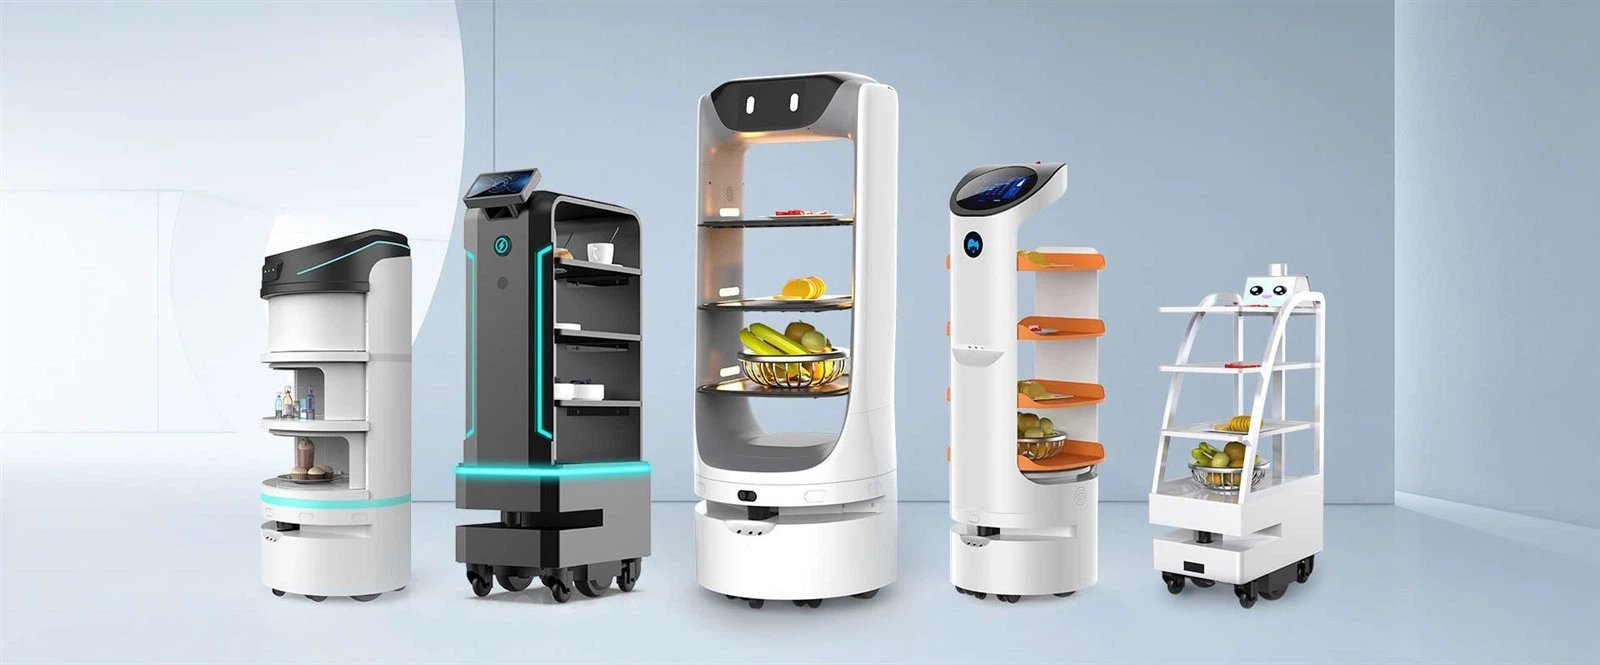
\includegraphics[width=\linewidth,height=3.0cm,keepaspectratio]{plat_restaurant.jpg}\\[3pt]
  {\small\textbf{Restaurant Delivery}\\
  e.g.\ Keenon T5\\
  Open shelves, \$1{,}700--3{,}000}
\end{minipage}\hfill
\begin{minipage}[t]{0.23\linewidth}\centering
  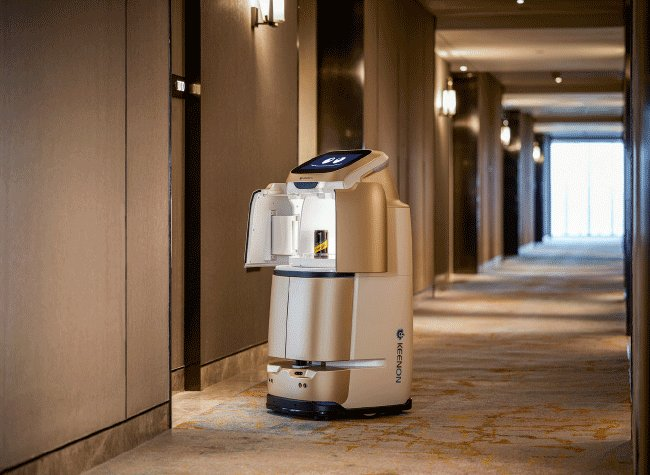
\includegraphics[width=\linewidth,height=3.0cm,keepaspectratio]{plat_hotel.jpg}\\[3pt]
  {\small\textbf{Hotel Delivery}\\
  Enclosed locking compartments\\
  PIN/QR access, elevator control}
\end{minipage}\hfill
\begin{minipage}[t]{0.23\linewidth}\centering
  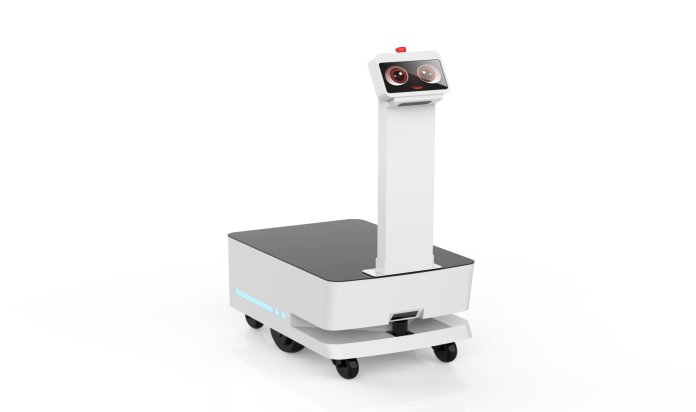
\includegraphics[width=\linewidth,height=3.0cm,keepaspectratio]{plat_factory.jpg}\\[3pt]
  {\small\textbf{Factory AMRs}\\
  100--1{,}000+\,kg payload\\
  Pallet lift, tow carts}
\end{minipage}

\caption{Service robot ecosystem. \textit{Top row}: chassis bases that expose open navigation APIs for developers to build on. \textit{Bottom row}: ready-to-use robots locked to a single industry vertical. Restaurant and hotel delivery robots are the most widely deployed service robot category globally. None of the ready-to-use categories offer an open interface for adding conversational AI, custom bodies, or research-level sensor access -- hence the chassis-base approach.}
\label{fig:landscape}
\end{figure}

\noindent The ready-to-use categories each serve a narrow purpose. Restaurant robots use open shelves and are optimised for crowded kitchen-to-table trips. Hotel robots carry enclosed locking compartments that only the correct guest can open via PIN or QR code, and can coordinate with building elevators. Reception robots are screen-focused and carry no payload. None of these matched the project requirement for a single platform combining autonomous navigation, conversational AI, item delivery, and telepresence at research-accessible cost.

Chassis bases expose raw navigation and sensor data for a developer to build upon. Six were evaluated in depth.

\subsubsection{Comparative Platform Evaluation}

Table~\ref{tab:platform_eval} summarises the six chassis platforms reviewed through their vendor documentation, ROS compatibility, payload ratings, sensor suites, and structural mounting options.

\begin{table}[H]
\centering
\small
\caption{Mobile chassis platforms evaluated for TAMRA.}
\label{tab:platform_eval}
\setlength{\tabcolsep}{4pt}
\begin{tabular}{@{} >{\raggedright\arraybackslash}p{2.8cm} r >{\raggedright\arraybackslash}p{1.5cm} >{\raggedright\arraybackslash}p{3.4cm} @{}}
\toprule
\textbf{Platform} & \textbf{USD} & \textbf{Payload} & \textbf{Verdict} \\
\midrule
Bao Xiaomi Mini    & 2{,}000 & Service only & Consumer-grade; no payload; closed nav \\
Reeman Moon Knight & 2{,}380 & 60\,kg       & Android SDK; limited open ROS support \\
\textbf{iMRP500}   & \textbf{1{,}550} & \textbf{50\,kg} & \textbf{Selected (AHP score 6.76)} \\
Wheeltec S100      & 1{,}250 & $\sim$15\,kg & Low payload; ROS~1 only; academic focus \\
Timo AI Robot      & 2{,}500 & Service only & Proprietary nav API; no raw data access \\
Uwant T5/T6        & 1{,}700 & 40\,kg       & Closed SLAM; no raw sensor access \\
\bottomrule
\end{tabular}
\end{table}

\noindent The iMRP500 scored highest under the AHP criteria from Chapter~4 (Reliability~47\%, Development Speed~30\%, Cost~15\%, Customisability~8\%). It was the only platform that combined a 50\,kg payload, an integrated industrial sensor suite with raw data accessible over a documented WebSocket protocol, and a circular footprint with structural mounting points for the body shell.

Before committing, the capability gap between TAMRA and the commercial hospital robots it is meant to compete with was assessed. Table~\ref{tab:commercial_comparison} shows where existing platforms fall short.

\begin{table}[H]
\centering
\small
\caption{Capability comparison with commercial hospital service robots.}
\label{tab:commercial_comparison}
\setlength{\tabcolsep}{4pt}
\begin{tabular}{@{} l c c c c r @{}}
\toprule
 & \textbf{Nav} & \textbf{Delivery} & \textbf{Voice AI} & \textbf{Telepres.} & \textbf{Price} \\
\midrule
PuduBot~2 \cite{pudubot2}         & \checkmark & \checkmark & --         & --         & \$12{,}000 \\
Keenon M2 \cite{m2medical}        & \checkmark & \checkmark & --         & --         & \$47{,}500 \\
Peanut Medical \cite{peanutmedical}& \checkmark & \checkmark & --         & \checkmark & \$12{,}700 \\
PUDU CC1 \cite{puducc1}           & \checkmark & --         & --         & --         & \$16{,}800 \\
\textbf{TAMRA}                    & \checkmark & \checkmark & \checkmark & \checkmark & \textbf{\$3{,}200} \\
\bottomrule
\end{tabular}
\end{table}

% -------------------------------------
\subsection{Hardware Implementation}
% -------------------------------------

\subsubsection{iMRP500 Chassis}

The iMRP500 is a circular differential-drive industrial chassis, 500\,mm in diameter, whose key specifications are given in Table~\ref{tab:imrp500_spec}. Procurement cost including shipping was 850\,OMR.

\begin{table}[H]
\centering
\small
\caption{iMRP500 chassis specifications.}
\label{tab:imrp500_spec}
\setlength{\tabcolsep}{5pt}
\begin{tabular}{@{} >{\raggedright\arraybackslash}p{3.8cm} >{\raggedright\arraybackslash}p{4.2cm} @{}}
\toprule
\textbf{Parameter} & \textbf{Value} \\
\midrule
Diameter / height      & 500\,mm / 310\,mm \\
Maximum payload        & 50\,kg \\
Drive                  & 2 servo hub motors, 5 wheels \\
LiDAR                  & TOF, 360$^{\circ}$, 20\,m range \\
Depth camera           & RGBD structured-light, 0.6--8\,m \\
IMU                    & 6-axis \\
Battery                & 24\,V / 20\,Ah Li-ion \\
Runtime (no load)      & 12\,h \\
Navigation accuracy    & $\pm$5\,cm \\
Max navigation speed   & 0.8\,m/s \\
Onboard compute        & Off-shelf SoC, Ubuntu 20.04 \\
Communication          & WebSocket port~9090, MJPEG port~9099 \\
Safety                 & Hardware E-stop (ISO~13850), soft-stop service \\
\bottomrule
\end{tabular}
\end{table}

\paragraph{Reverse-engineering the communication layer.}
The chassis ships with a proprietary operator application and a Chinese-language protocol document. Commissioning it for research required mapping the full ROS topic and service graph over the WebSocket bridge. The following sensor topics were confirmed and integrated:

\begin{itemize}
  \item \texttt{/scan} -- 360$^{\circ}$ TOF LiDAR scan, primary localisation input
  \item \texttt{/upcamera/rgb/image\_raw} and \texttt{/upcamera/depth/image\_raw} -- RGBD camera mounted pointing upward to detect overhead obstacles (counter overhangs, low tables)
  \item \texttt{/robot\_pose} -- fused position estimate $(x,\,y,\,\theta)$
  \item \texttt{/robot\_status} -- battery percentage, charger state, navigation status code
  \item \texttt{/mobile\_base/sensors/core} -- wheel encoder odometry, ultrasonic proximity (3-point frontal)
  \item \texttt{/localization\_confidence} -- real-time localisation quality score (0.0--1.0)
\end{itemize}

\noindent Navigation goals are dispatched via the \texttt{/poi} service using named waypoints stored in the chassis map database. The navigation stack is built on Nav2 \cite{macenski2023nav2}. The localisation stack fuses three complementary sources. Let $\mathbf{x}_t = [x,\,y,\,\theta]^T$ be the robot pose at time $t$. An extended Kalman filter \cite{thrun2005probabilistic} operates in two steps:
\begin{align}
  \textit{Predict:}\quad & \hat{\mathbf{x}}_{t}^{-} = f(\mathbf{x}_{t-1},\,\mathbf{u}_t) \\[4pt]
  \textit{Update:}\quad  & \hat{\mathbf{x}}_{t} = \hat{\mathbf{x}}_{t}^{-}
    + \mathbf{K}_t\!\left(\mathbf{z}_t^{\text{LiDAR}} - h\!\left(\hat{\mathbf{x}}_{t}^{-}\right)\right)
\end{align}
where $\mathbf{u}_t$ encodes wheel encoder and IMU data, $\mathbf{z}_t^{\text{LiDAR}}$ is the scan-match observation, $h(\cdot)$ is the observation model, and $\mathbf{K}_t$ is the Kalman gain. The costmap runs four stacked layers: a LiDAR obstacle layer (4\,m range, 0.6\,m max height), an upward-camera layer for overhead detection (3.5\,m range, 2\,m max height), a downward-camera layer, and an inflation layer (0.8\,m radius, scaling factor~10). The local costmap updates at 8\,Hz over a $3\times3$\,m window at 0.03\,m resolution; the global costmap at 4\,Hz over $10\times10$\,m at 0.05\,m resolution.

\paragraph{Internal architecture.}
Physical inspection of the chassis electronics revealed how the manufacturer achieved its cost point. Three layers are present: the bottom layer uses commodity CNC stepper motor drivers (identifiable by their green terminal blocks and PWR/ALM LED indicators); the mid layer is an off-the-shelf SoC board with USB and Ethernet ports; the top layer uses sensor interface boards from the 3D-printer ecosystem. The drive motors are hub motors from the electric scooter supply chain. This architecture substitutes widely available commodity components for custom ASICs, reducing cost without sacrificing reliability at service-robot duty cycles.

\begin{figure}[H]
  \centering
  \begin{minipage}[t]{0.48\linewidth}
    \centering
    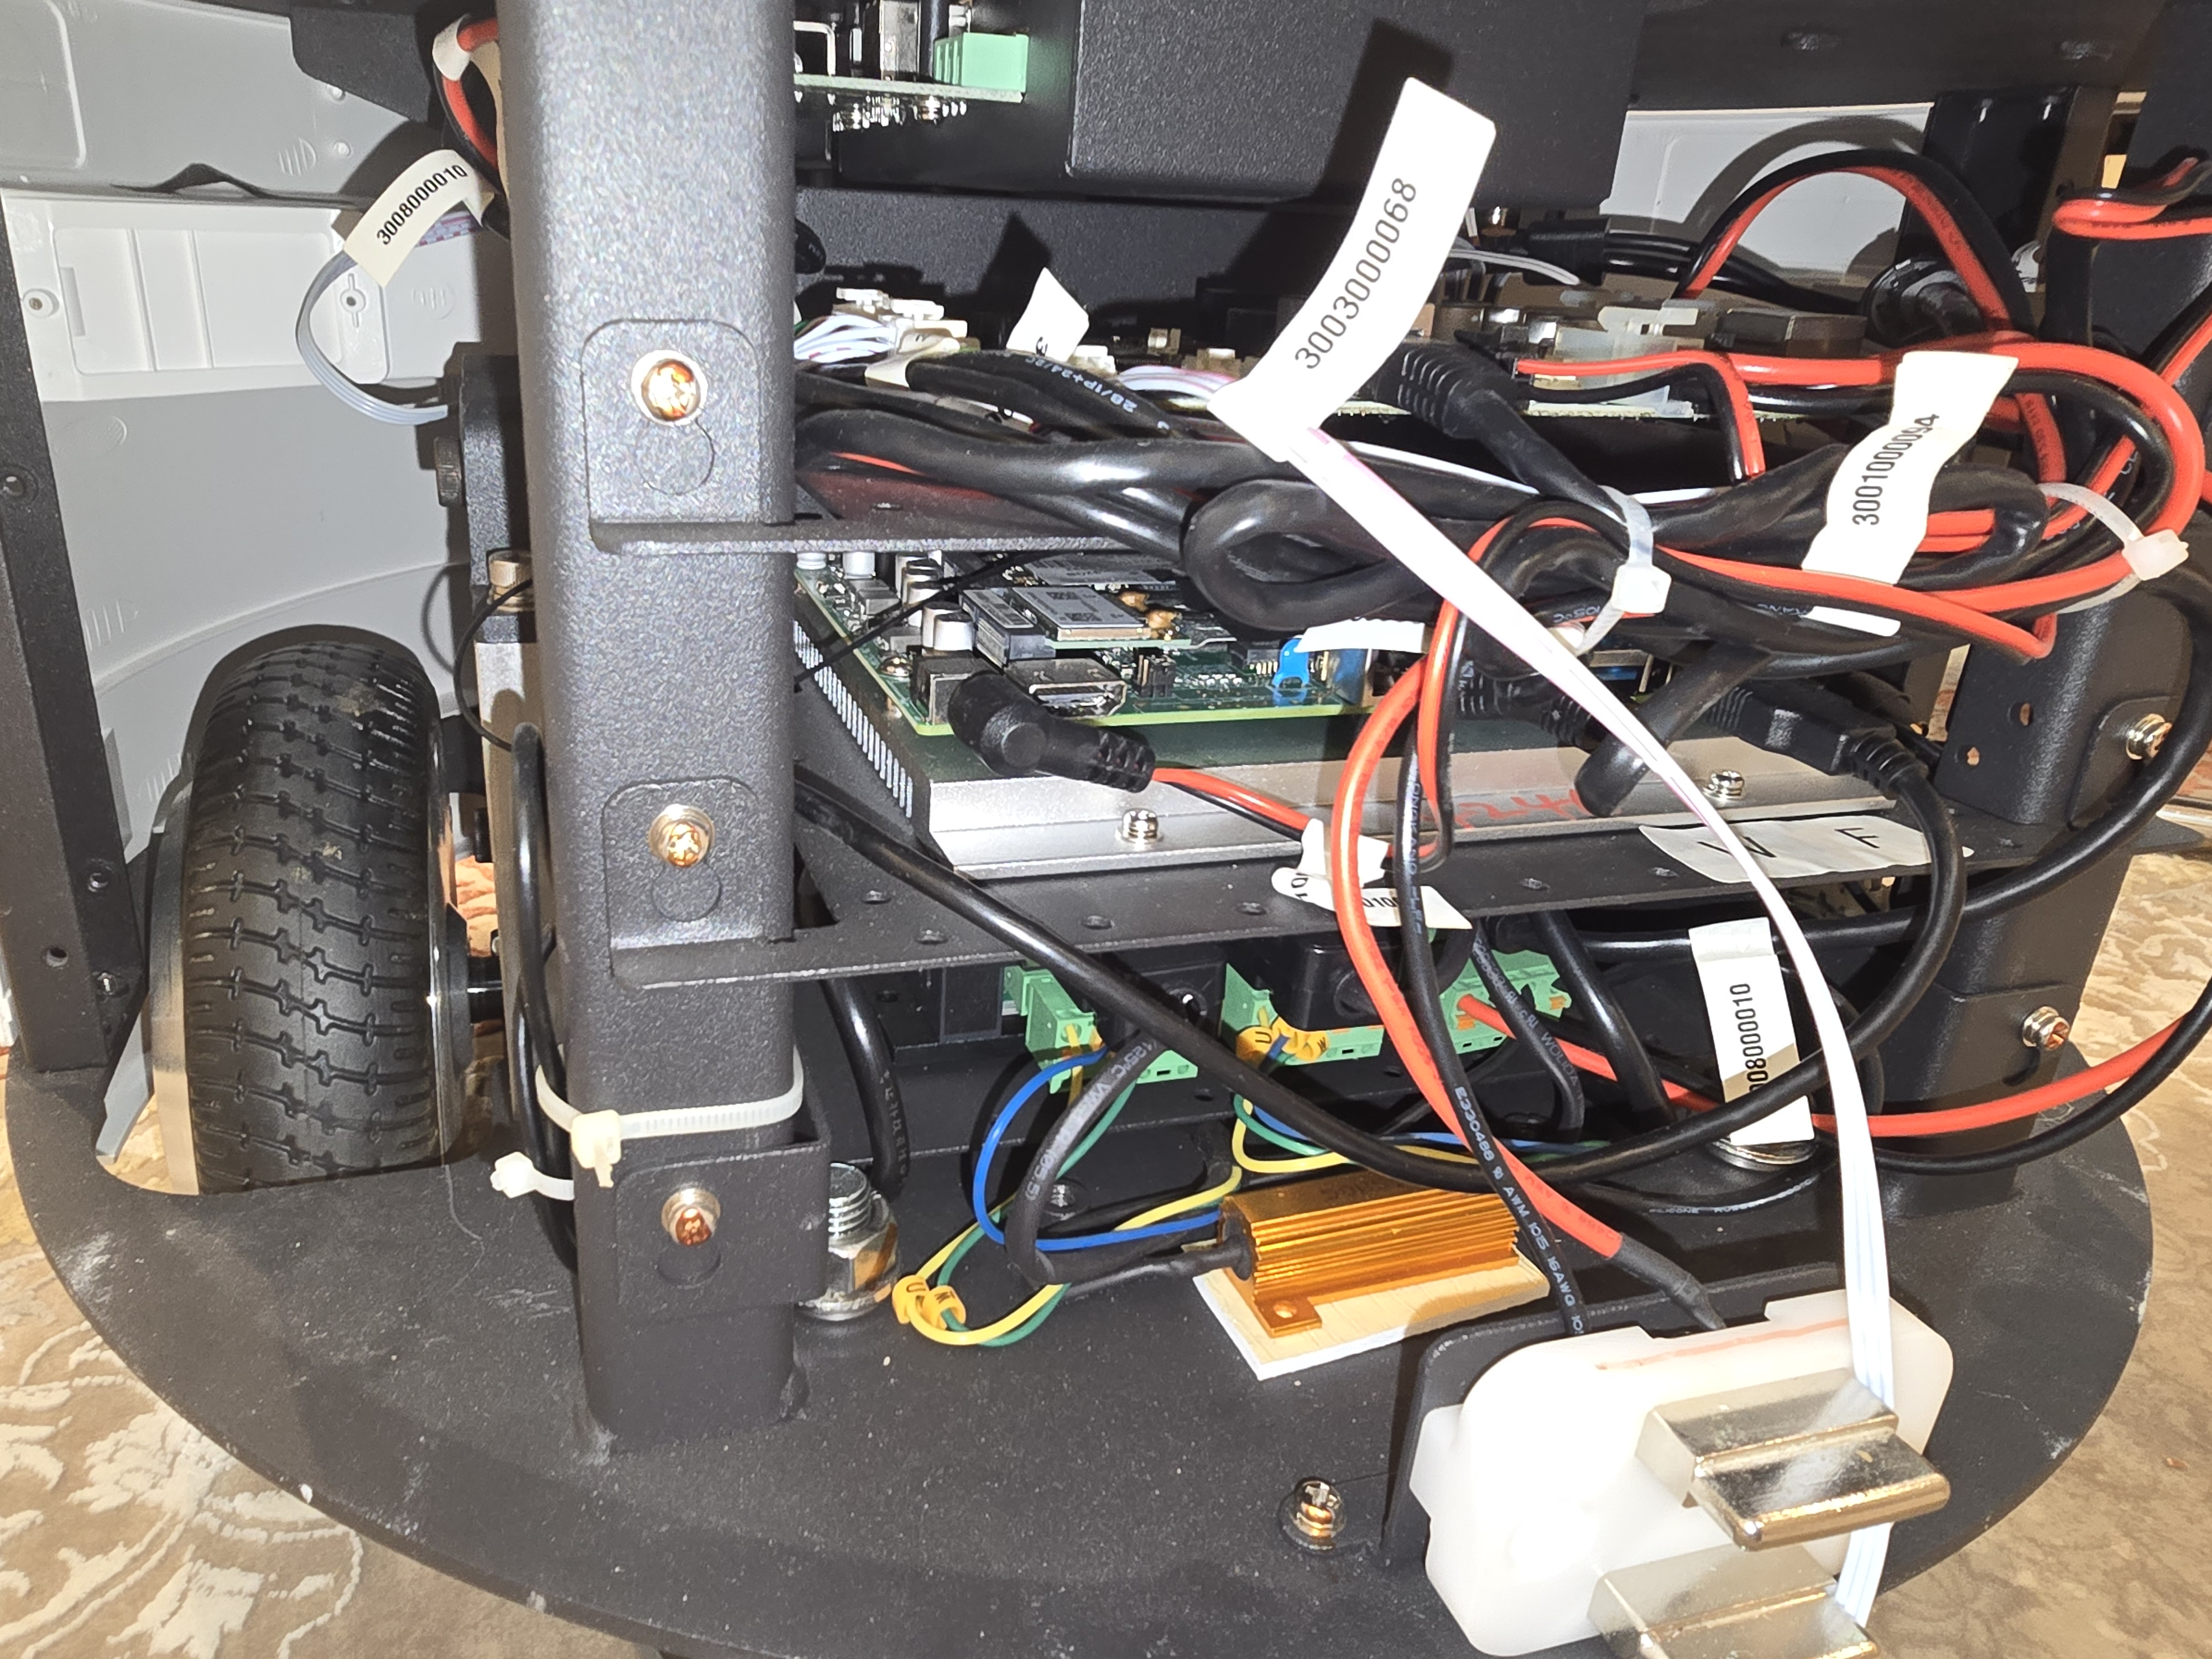
\includegraphics[width=\linewidth,height=5.5cm,keepaspectratio]{internals1.jpeg}
  \end{minipage}\hfill
  \begin{minipage}[t]{0.48\linewidth}
    \centering
    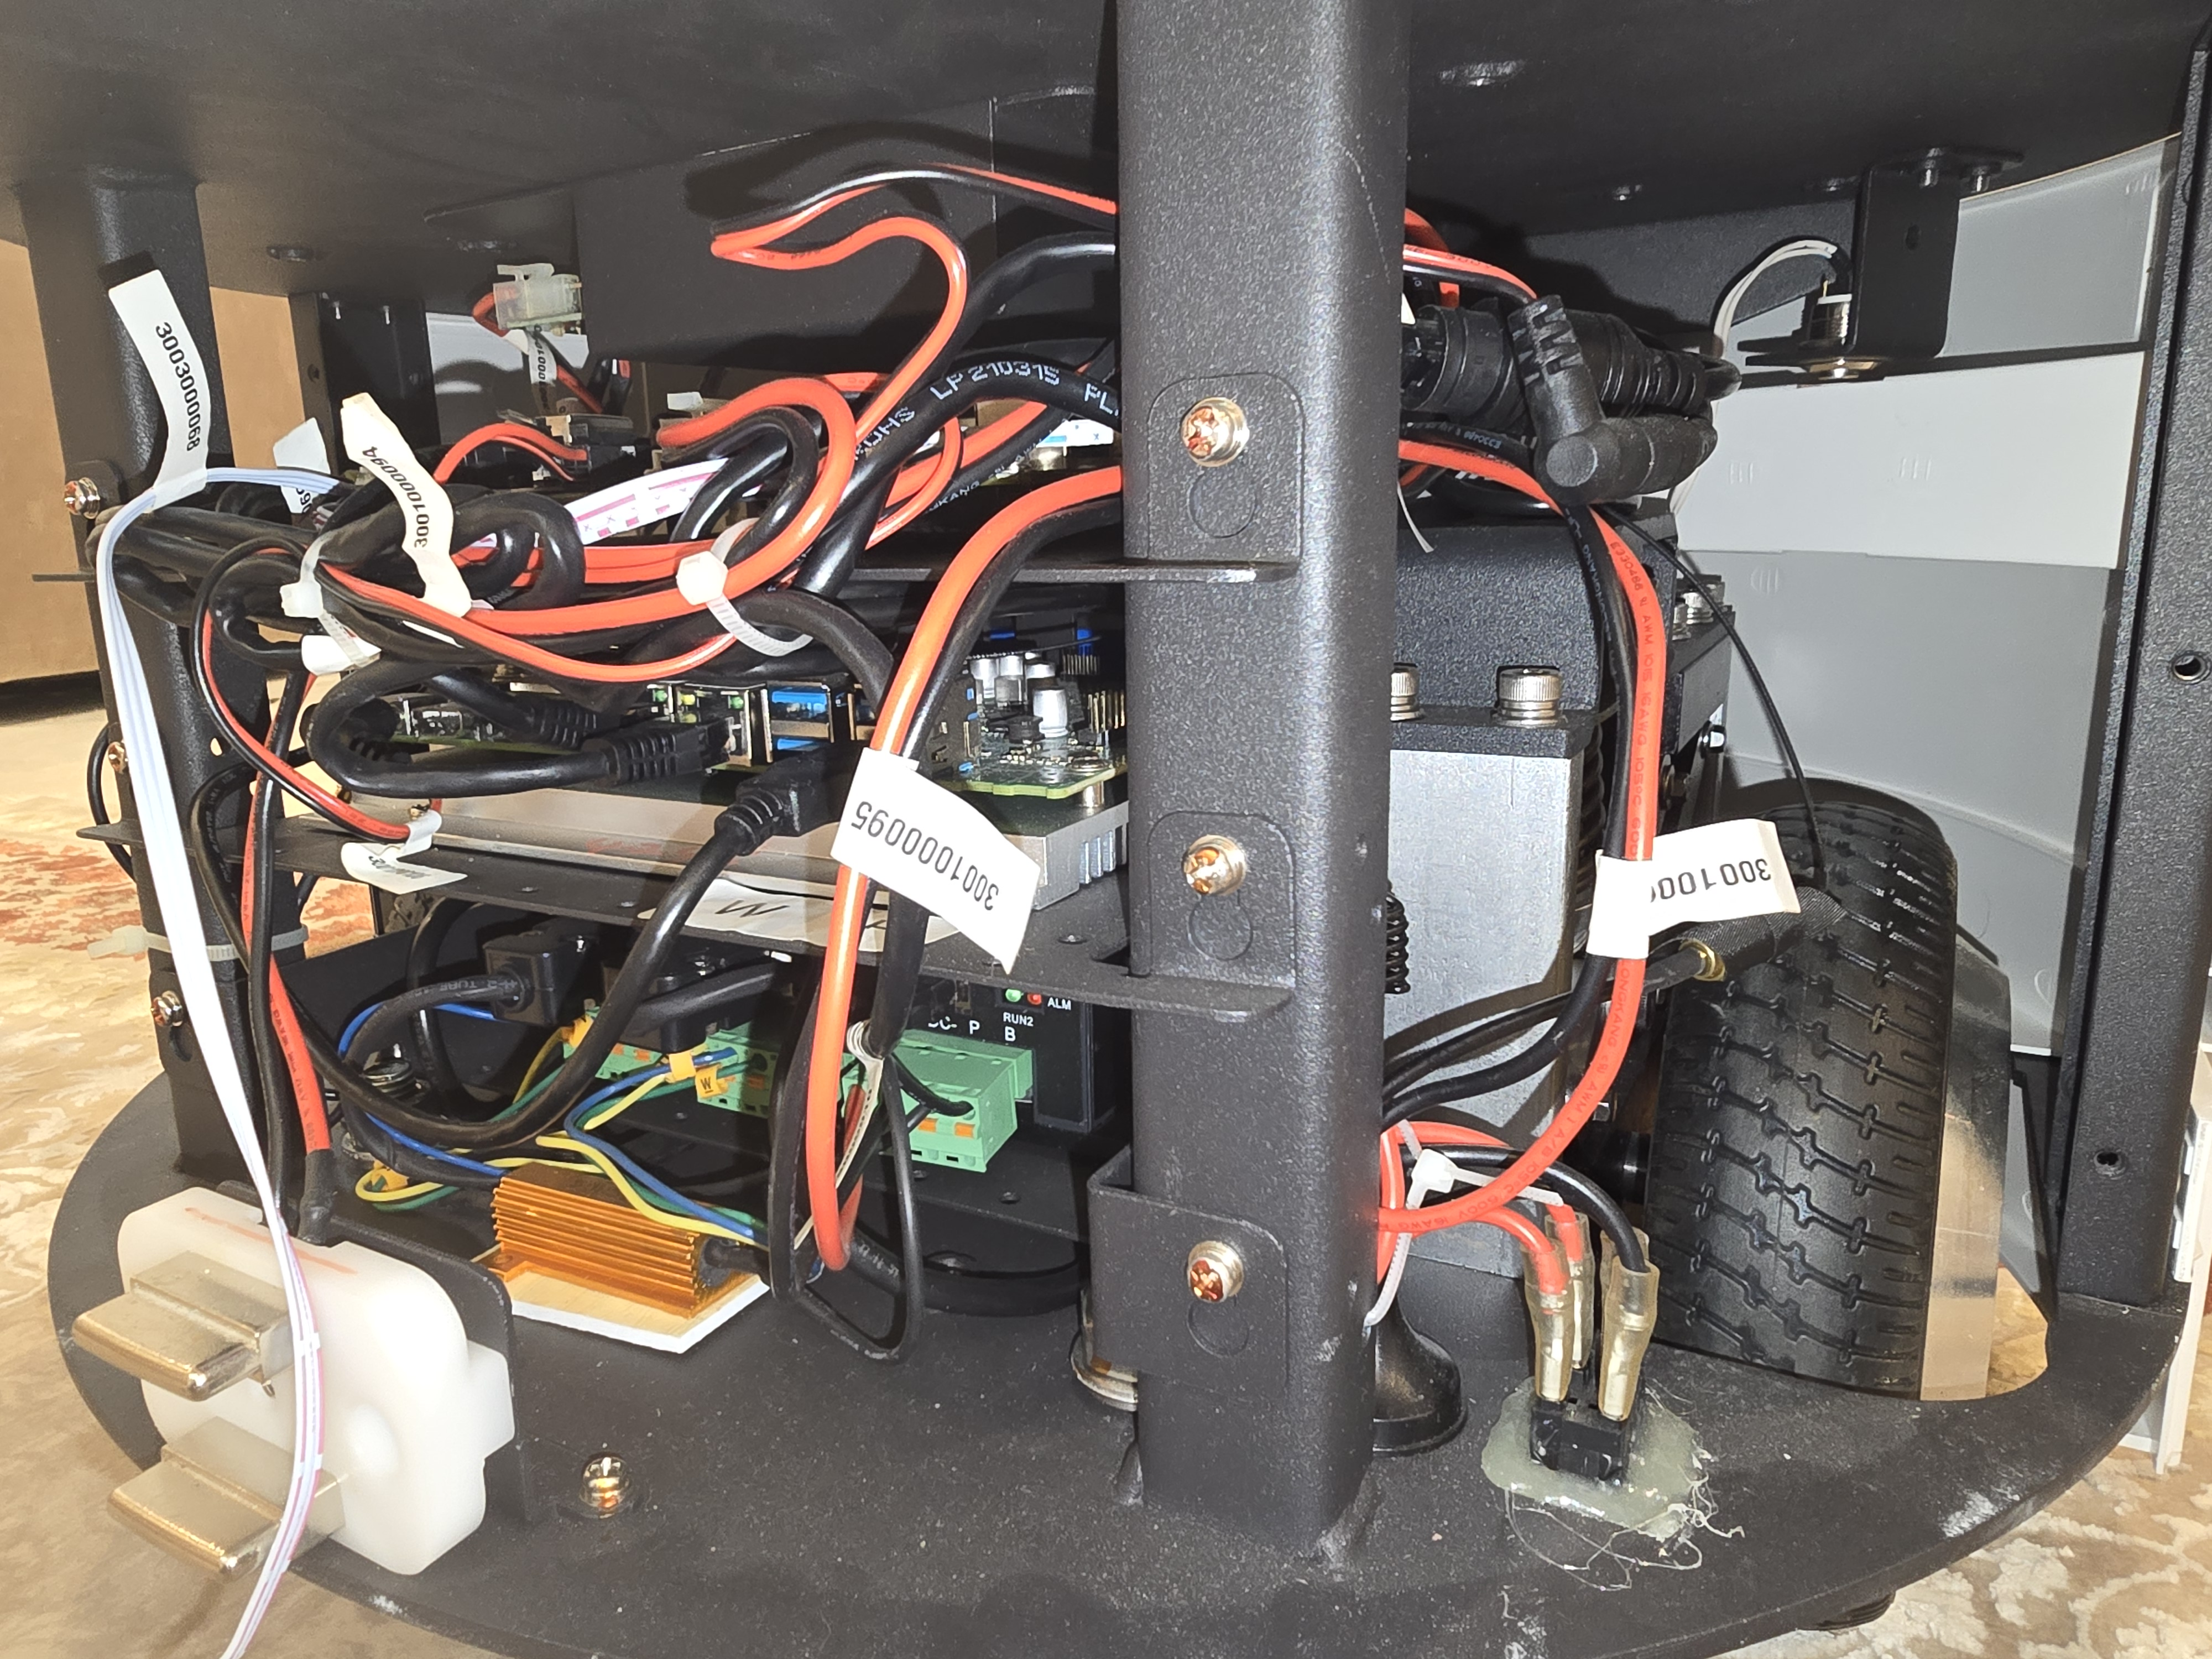
\includegraphics[width=\linewidth,height=5.5cm,keepaspectratio]{internals2.jpeg}
  \end{minipage}
  \caption{iMRP500 internal electronics: commodity CNC stepper drivers (bottom), off-the-shelf SoC (mid), and 3D-printer-style sensor boards (top). Scooter hub motors are visible at the periphery.}
  \label{fig:internals}
\end{figure}

\subsubsection{Body Shell Design and Fabrication}

The body shell connects the 500\,mm circular chassis to the robot's human-facing components: the display, the storage compartment, and the exterior surface that patients and staff interact with. Eleven functional requirements constrained the design:

\begin{itemize}
  \item Display tilted at 40$^{\circ}$ from horizontal for ergonomic use at standing and seated heights \cite{frontiers2024}
  \item Display recess accepting a future larger screen without structural change (5\,mm step, $360\times260$\,mm outer frame)
  \item Internal tray for secure transport; external storage compartment for accessible delivery
  \item Footprint within the 500\,mm chassis diameter (LiDAR clearance requirement)
  \item Added mass not exceeding 12\,kg (chassis centre-of-mass stability limit)
  \item Total height not exceeding 1{,}100\,mm (tipping stability per chassis datasheet)
  \item Hospital-compatible materials: no sharp edges, surfaces compatible with standard disinfectant protocols \cite{intel2024}
  \item Concealed cable routing between tablet, display driver, and chassis
  \item Manufacturable in Oman using locally available trades
  \item Budget not exceeding 300\,OMR
  \item Warm, approachable aesthetic to reduce patient anxiety \cite{beran2013}
\end{itemize}

\paragraph{Design workflow.}
The shell was developed in three stages. First, concept rendering was used to rapidly explore aesthetic directions. Hundreds of configurations were reviewed within hours -- far faster than equivalent CAD iteration -- converging on a tapered silhouette with a central wood-veneer accent panel, a recessed display at the top, and a rear storage compartment.

Second, the selected concept image was fed into an AI-based 3D mesh generator (Hunyuan3D~v3.1), producing an initial mesh that captured the organic curvature but contained fabrication-incompatible geometry: overhangs beyond the 500\,mm radius and incorrect storage proportions.

Third, the mesh was used as a geometric reference for parametric reconstruction in Autodesk Fusion~360, producing fabrication-ready engineering drawings with tolerances. Final dimensions: 900\,mm total height, 500\,mm base (chassis interface), 400\,mm waist, 210\,mm storage depth, 40$^{\circ}$ display tilt.

\begin{figure}[H]
  \centering
  \begin{minipage}[t]{0.36\linewidth}
    \centering
    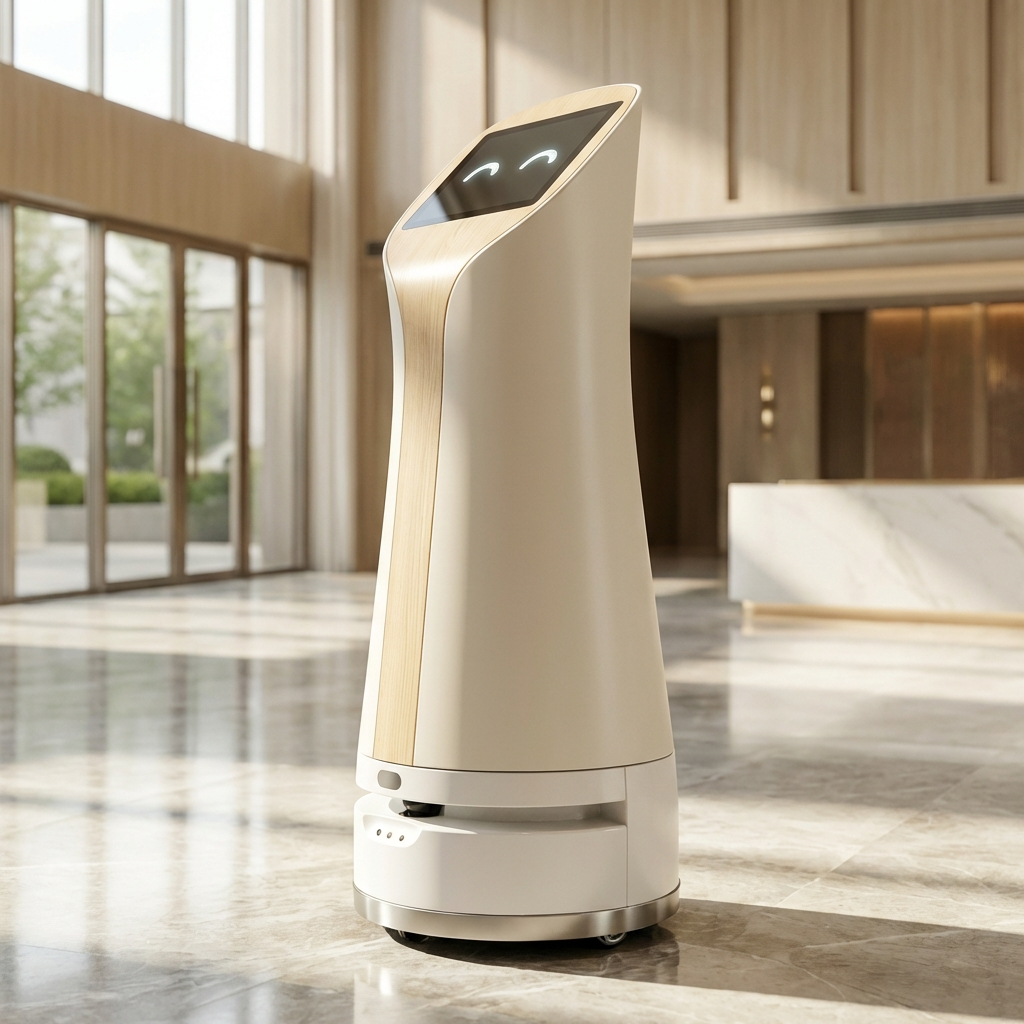
\includegraphics[width=\linewidth]{render_front.jpeg}
    \caption*{(a) Concept render}
  \end{minipage}\hfill
  \begin{minipage}[t]{0.60\linewidth}
    \centering
    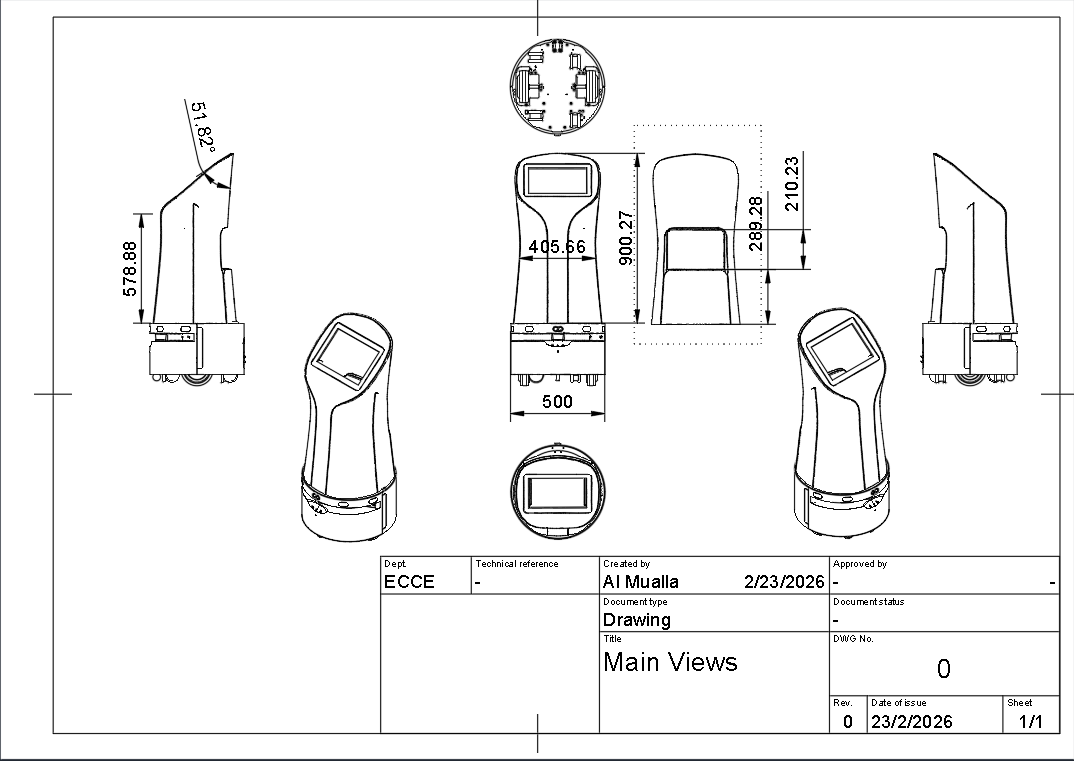
\includegraphics[width=\linewidth]{engn_drawing_robot_dimensions.png}
    \caption*{(b) Fusion~360 engineering drawing}
  \end{minipage}
  \caption{Body shell design workflow: concept render (left) and parametric engineering drawing with fabrication dimensions (right). The 500\,mm base diameter matches the chassis footprint exactly, preserving LiDAR clearance on all sides.}
  \label{fig:design_to_drawing}
\end{figure}

\paragraph{Material selection.}
Several manufacturing routes were evaluated:

\begin{itemize}
  \item \textbf{3D printing} -- rejected: cost-prohibitive for large curved panels, slow for the timeline.
  \item \textbf{Fibreglass composite layup} -- viable but requires specialist skills not locally available at reasonable cost.
  \item \textbf{CNC-machined foam} -- explored seriously. High-density polyurethane foam, when CNC-machined and finished, produces complex curved surfaces that are visually indistinguishable from moulded plastic or fibreglass. The technique is widely used in film set construction and commercial display fabrication. The team consulted a local Omani foam artist supplying a major regional perfume brand. The result quality was high (Figure~\ref{fig:foam}), but materials and machining costs reached approximately 400\,OMR -- exceeding the body shell budget -- and was therefore set aside.
  \item \textbf{MDF with oak veneer} -- selected: widely available, shaped by local carpenters in Muscat, lightweight, and finishes to a warm surface compatible with clinical-grade disinfectant wipes.
  \item \textbf{Acrylic sheet} -- selected for the display surround: dimensionally precise, smooth, and cleanable.
\end{itemize}

\begin{figure}[H]
  \centering
  \begin{minipage}[t]{0.48\linewidth}
    \centering
    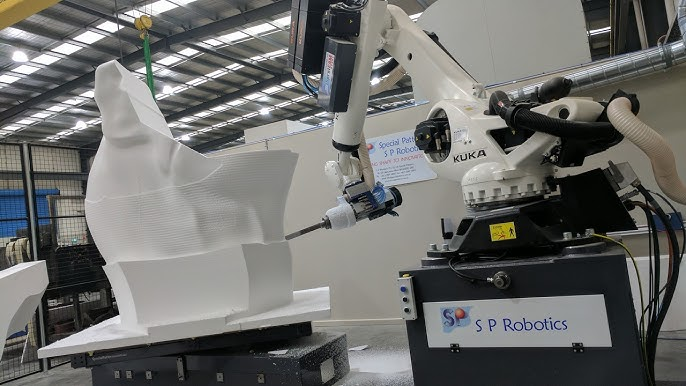
\includegraphics[width=\linewidth,height=5cm,keepaspectratio]{foam_cnc.jpg}
    \caption*{(a) CNC robot machining foam (S P Robotics)}
  \end{minipage}\hfill
  \begin{minipage}[t]{0.48\linewidth}
    \centering
    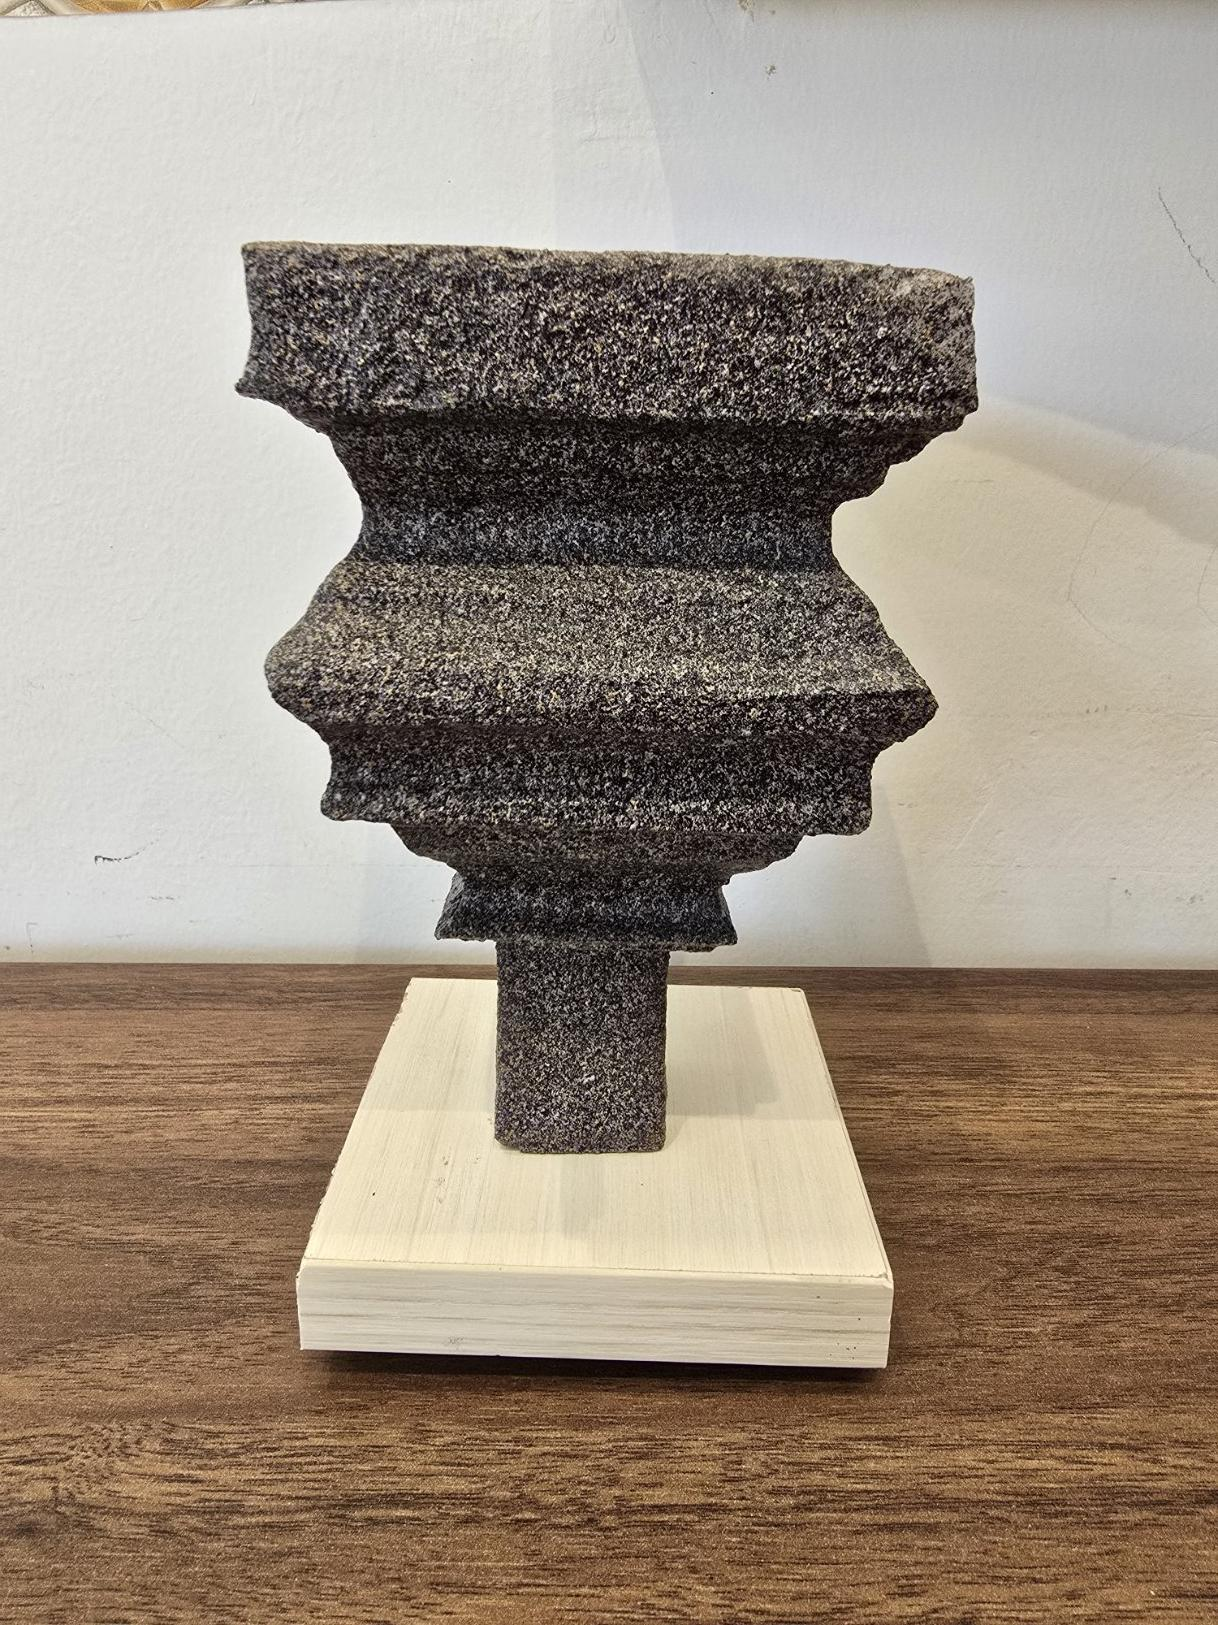
\includegraphics[width=\linewidth,height=5cm,keepaspectratio]{foam_sample.jpg}
    \caption*{(b) Small foam sculpture built as a hands-on learning exercise to understand the material}
  \end{minipage}
  \caption{CNC-machined polyurethane foam: the technique produces surfaces indistinguishable from moulded plastic or fibreglass and was explored as a body shell option. Material and machining costs in Oman ($\approx$400\,OMR) placed it above the body shell budget.}
  \label{fig:foam}
\end{figure}

\paragraph{Fabrication sequence.}
The MDF subframe was cut and assembled at a carpentry workshop in Muscat. Figures~\ref{fig:fab_sequence} and~\ref{fig:final_robot} document the process from skeleton to finished robot.

\begin{figure}[H]
  \centering
  \begin{minipage}[t]{0.32\linewidth}
    \centering
    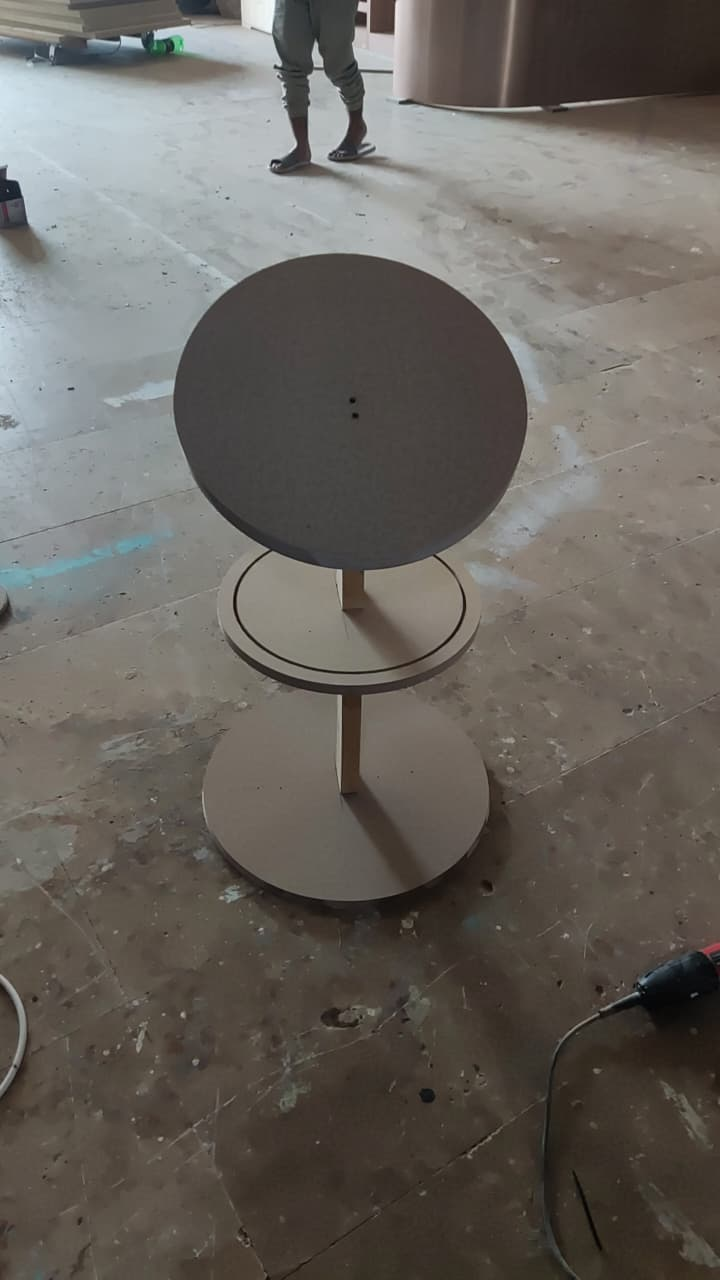
\includegraphics[width=\linewidth,height=5cm,keepaspectratio]{fab_step1.jpeg}
    \caption*{(a) MDF circular decks forming the structural skeleton}
  \end{minipage}\hfill
  \begin{minipage}[t]{0.32\linewidth}
    \centering
    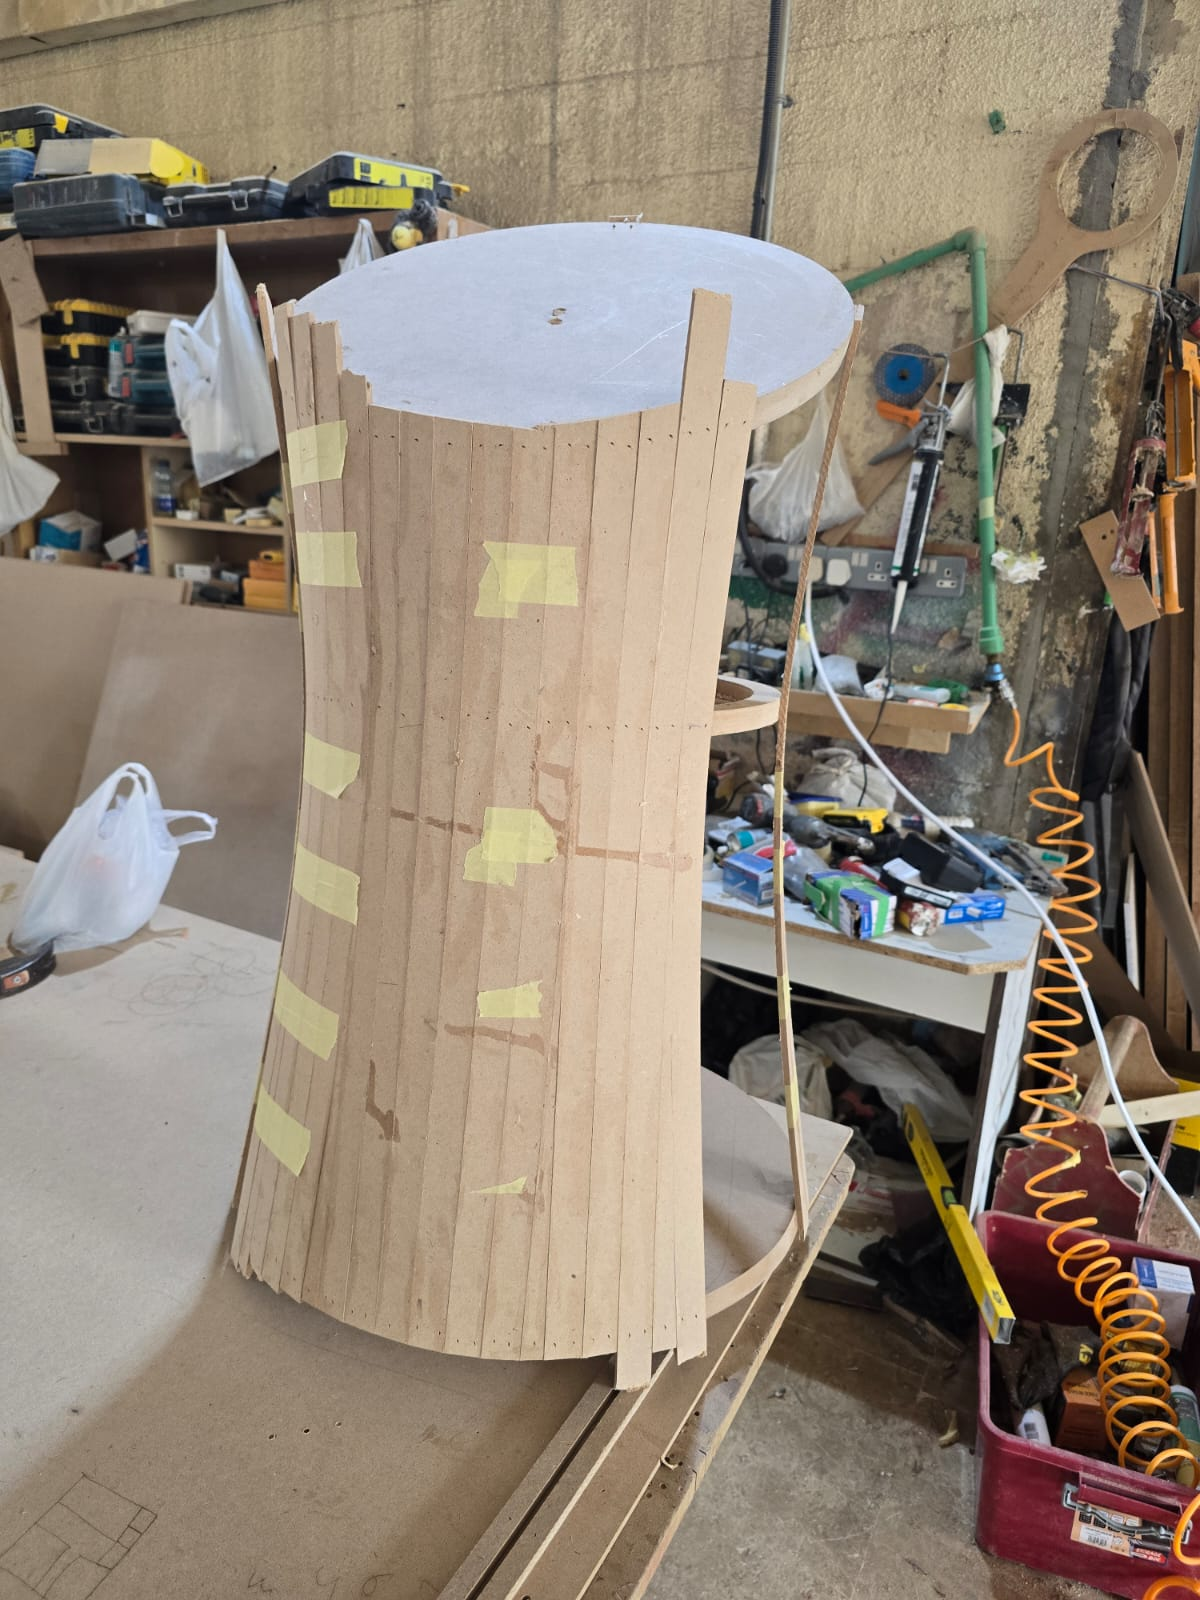
\includegraphics[width=\linewidth,height=5cm,keepaspectratio]{fab_step3.jpeg}
    \caption*{(b) Thin MDF strips bent and laminated around the skeleton}
  \end{minipage}\hfill
  \begin{minipage}[t]{0.32\linewidth}
    \centering
    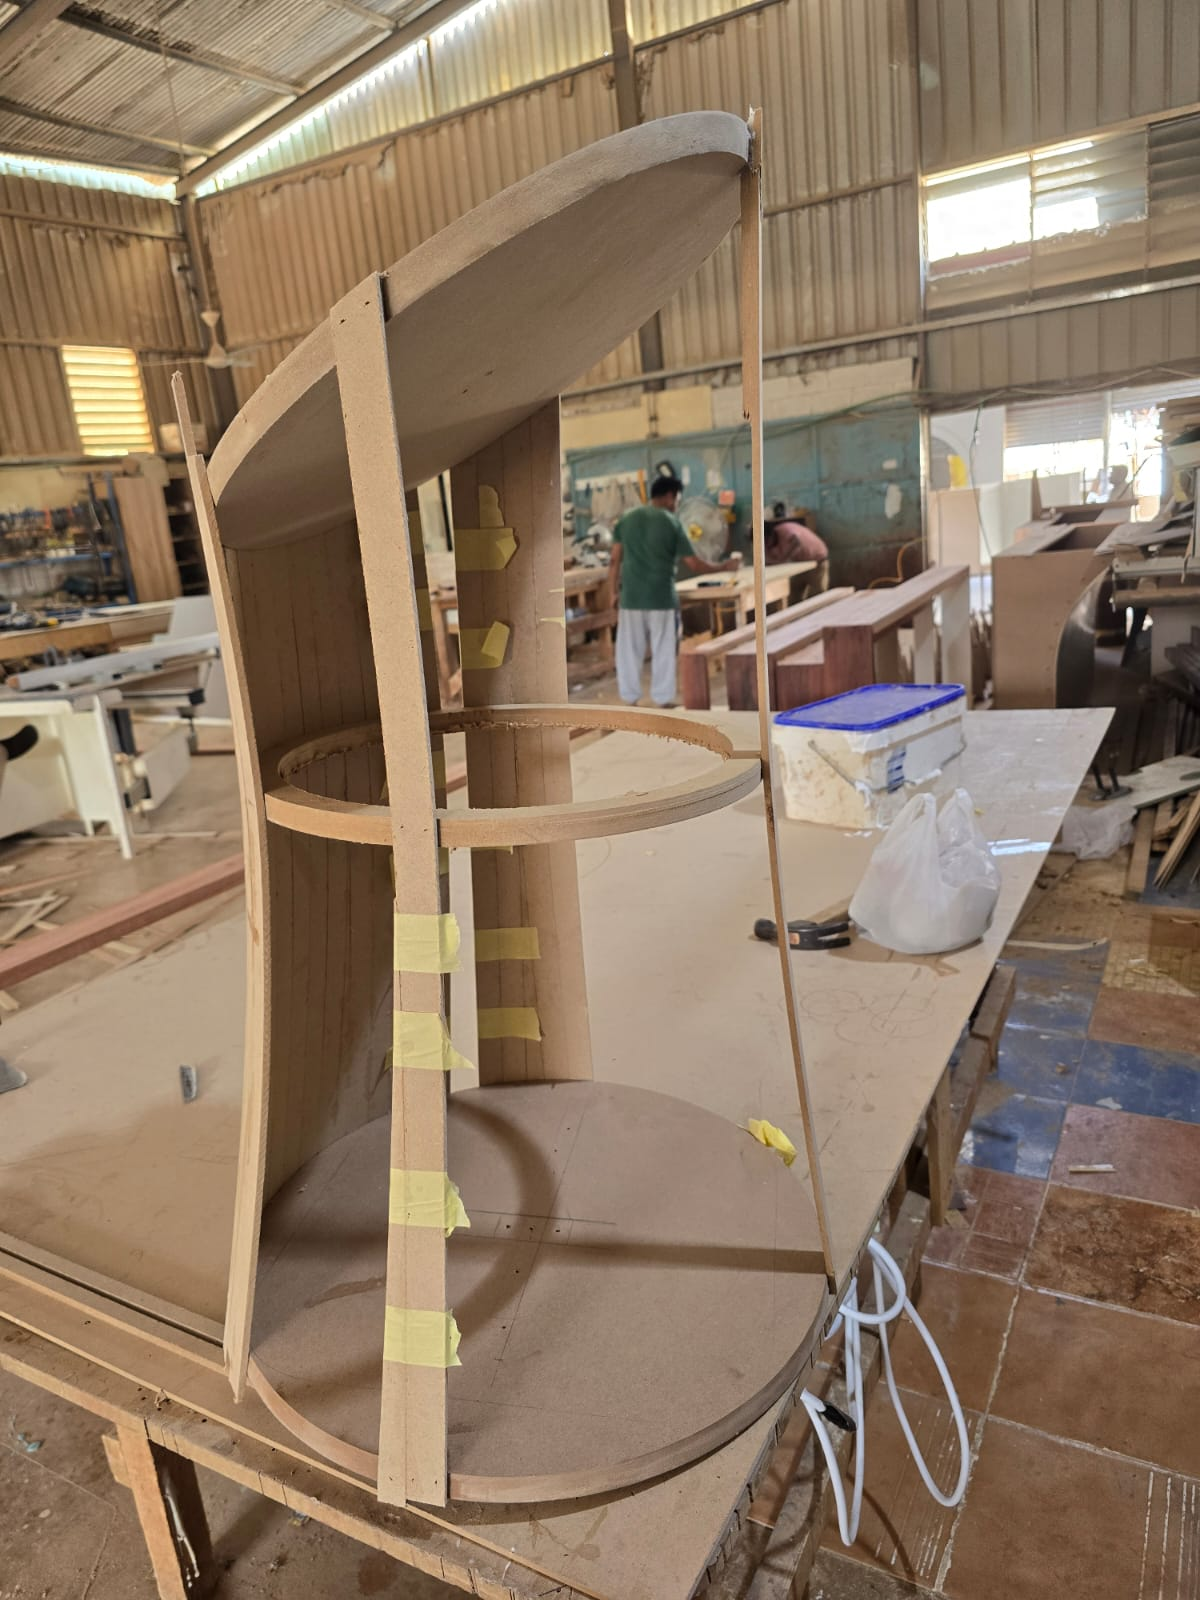
\includegraphics[width=\linewidth,height=5cm,keepaspectratio]{fab_step2.jpeg}
    \caption*{(c) Storage bay and upper frame fitted}
  \end{minipage}
  \caption{Body shell fabrication sequence. MDF circular decks set the profile at each level (a). Thin vertical strips are wetted and bent around the skeleton then laminated to form the curved surface (b and c, same stage shown from different angles).}
  \label{fig:fab_sequence}
\end{figure}

\begin{figure}[H]
  \centering
  \begin{minipage}[t]{0.32\linewidth}
    \centering
    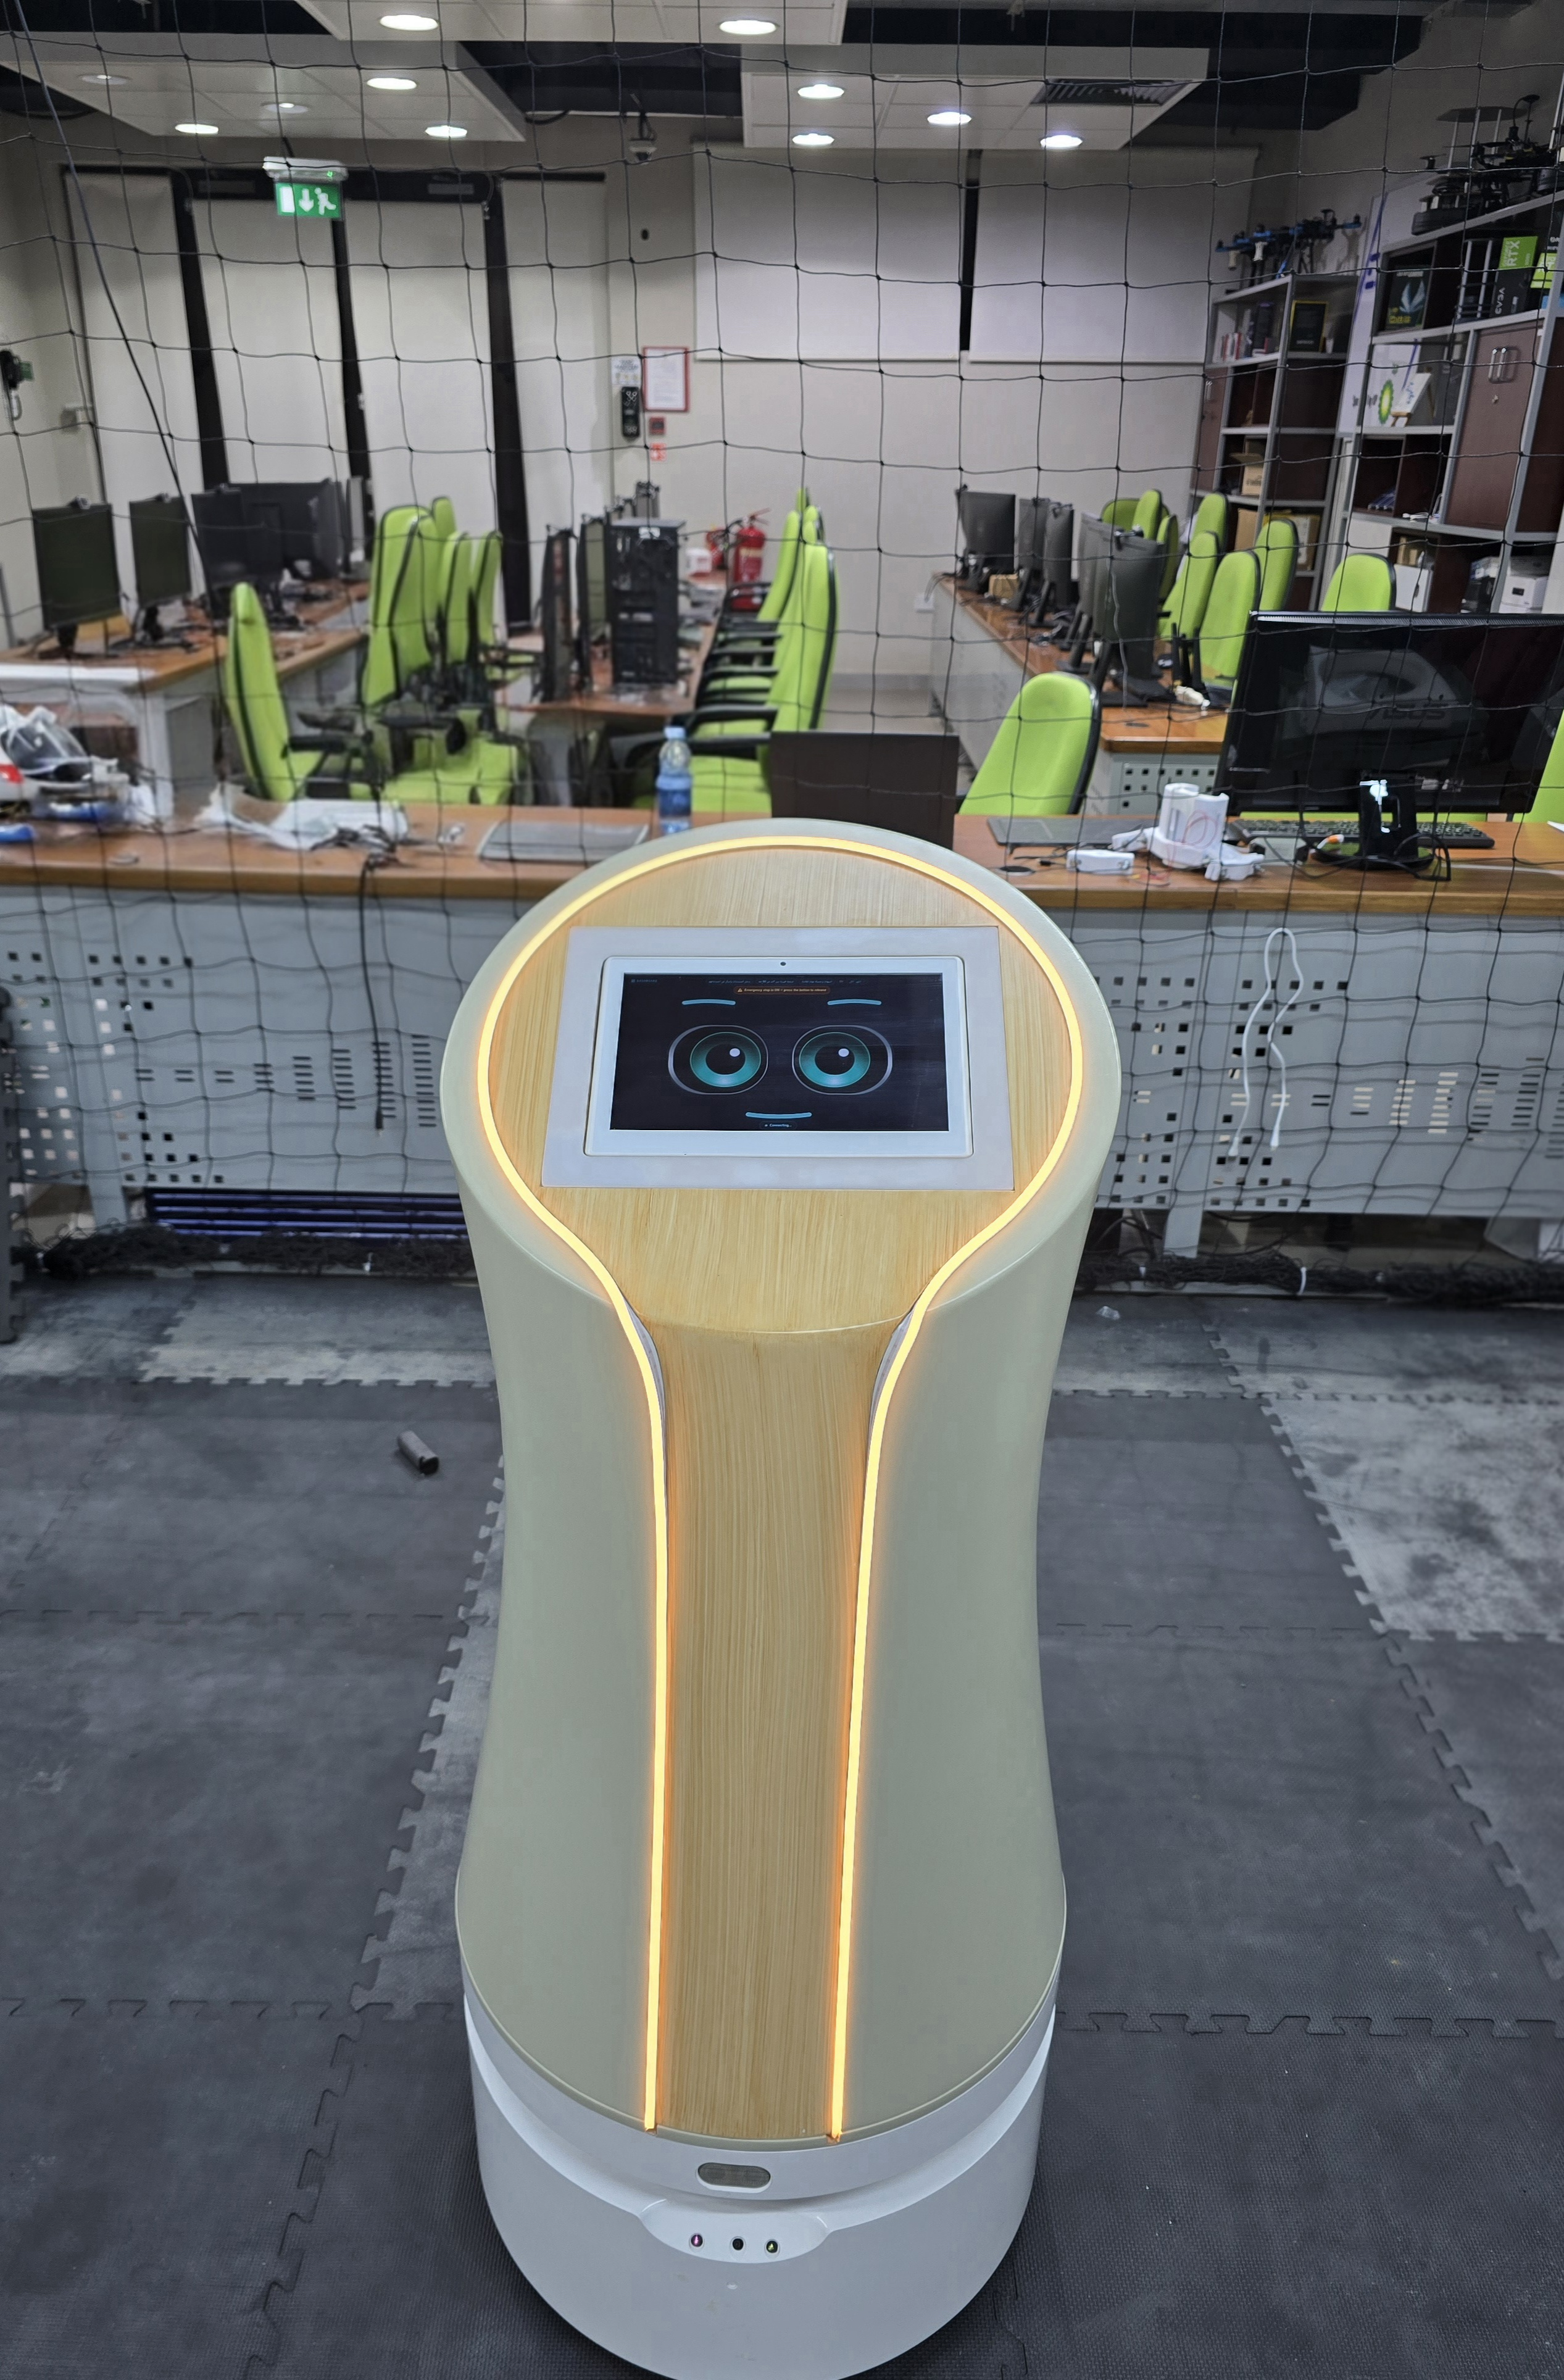
\includegraphics[width=\linewidth,height=6.5cm,keepaspectratio]{robot_front.jpg}
    \caption*{(a) Front view}
  \end{minipage}\hfill
  \begin{minipage}[t]{0.32\linewidth}
    \centering
    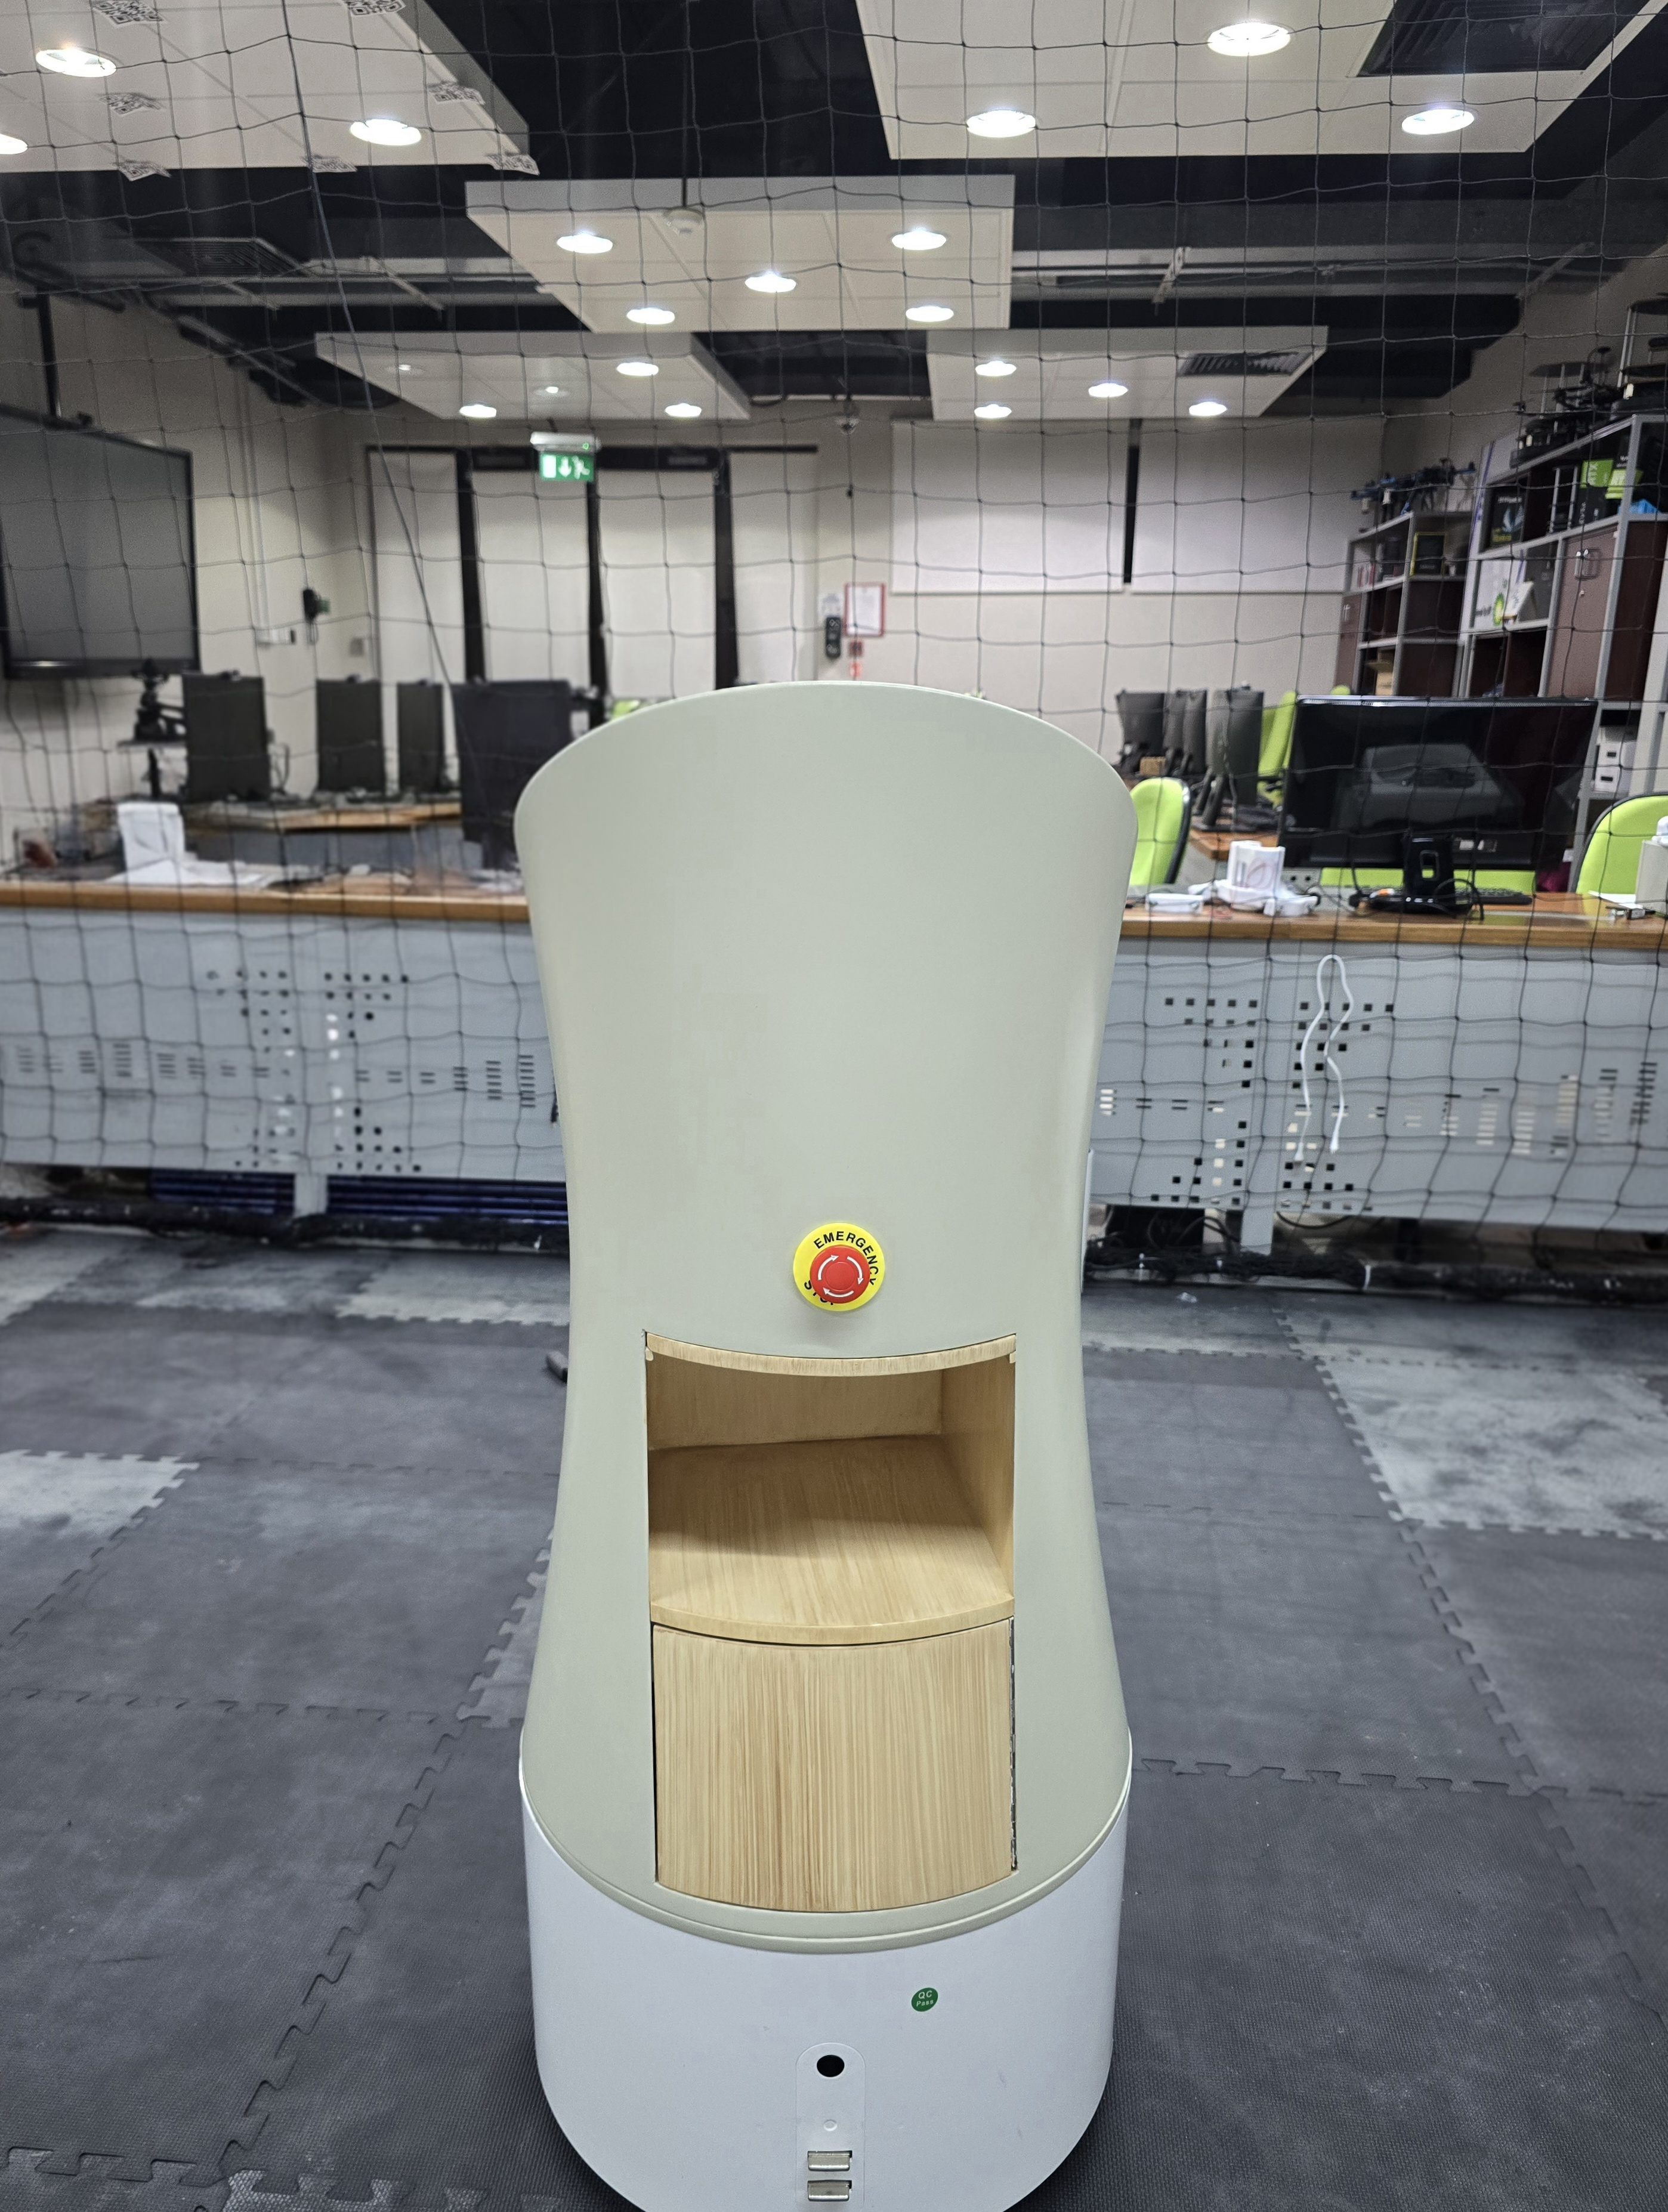
\includegraphics[width=\linewidth,height=6.5cm,keepaspectratio]{robot_rear.jpg}
    \caption*{(b) Rear view}
  \end{minipage}\hfill
  \begin{minipage}[t]{0.32\linewidth}
    \centering
    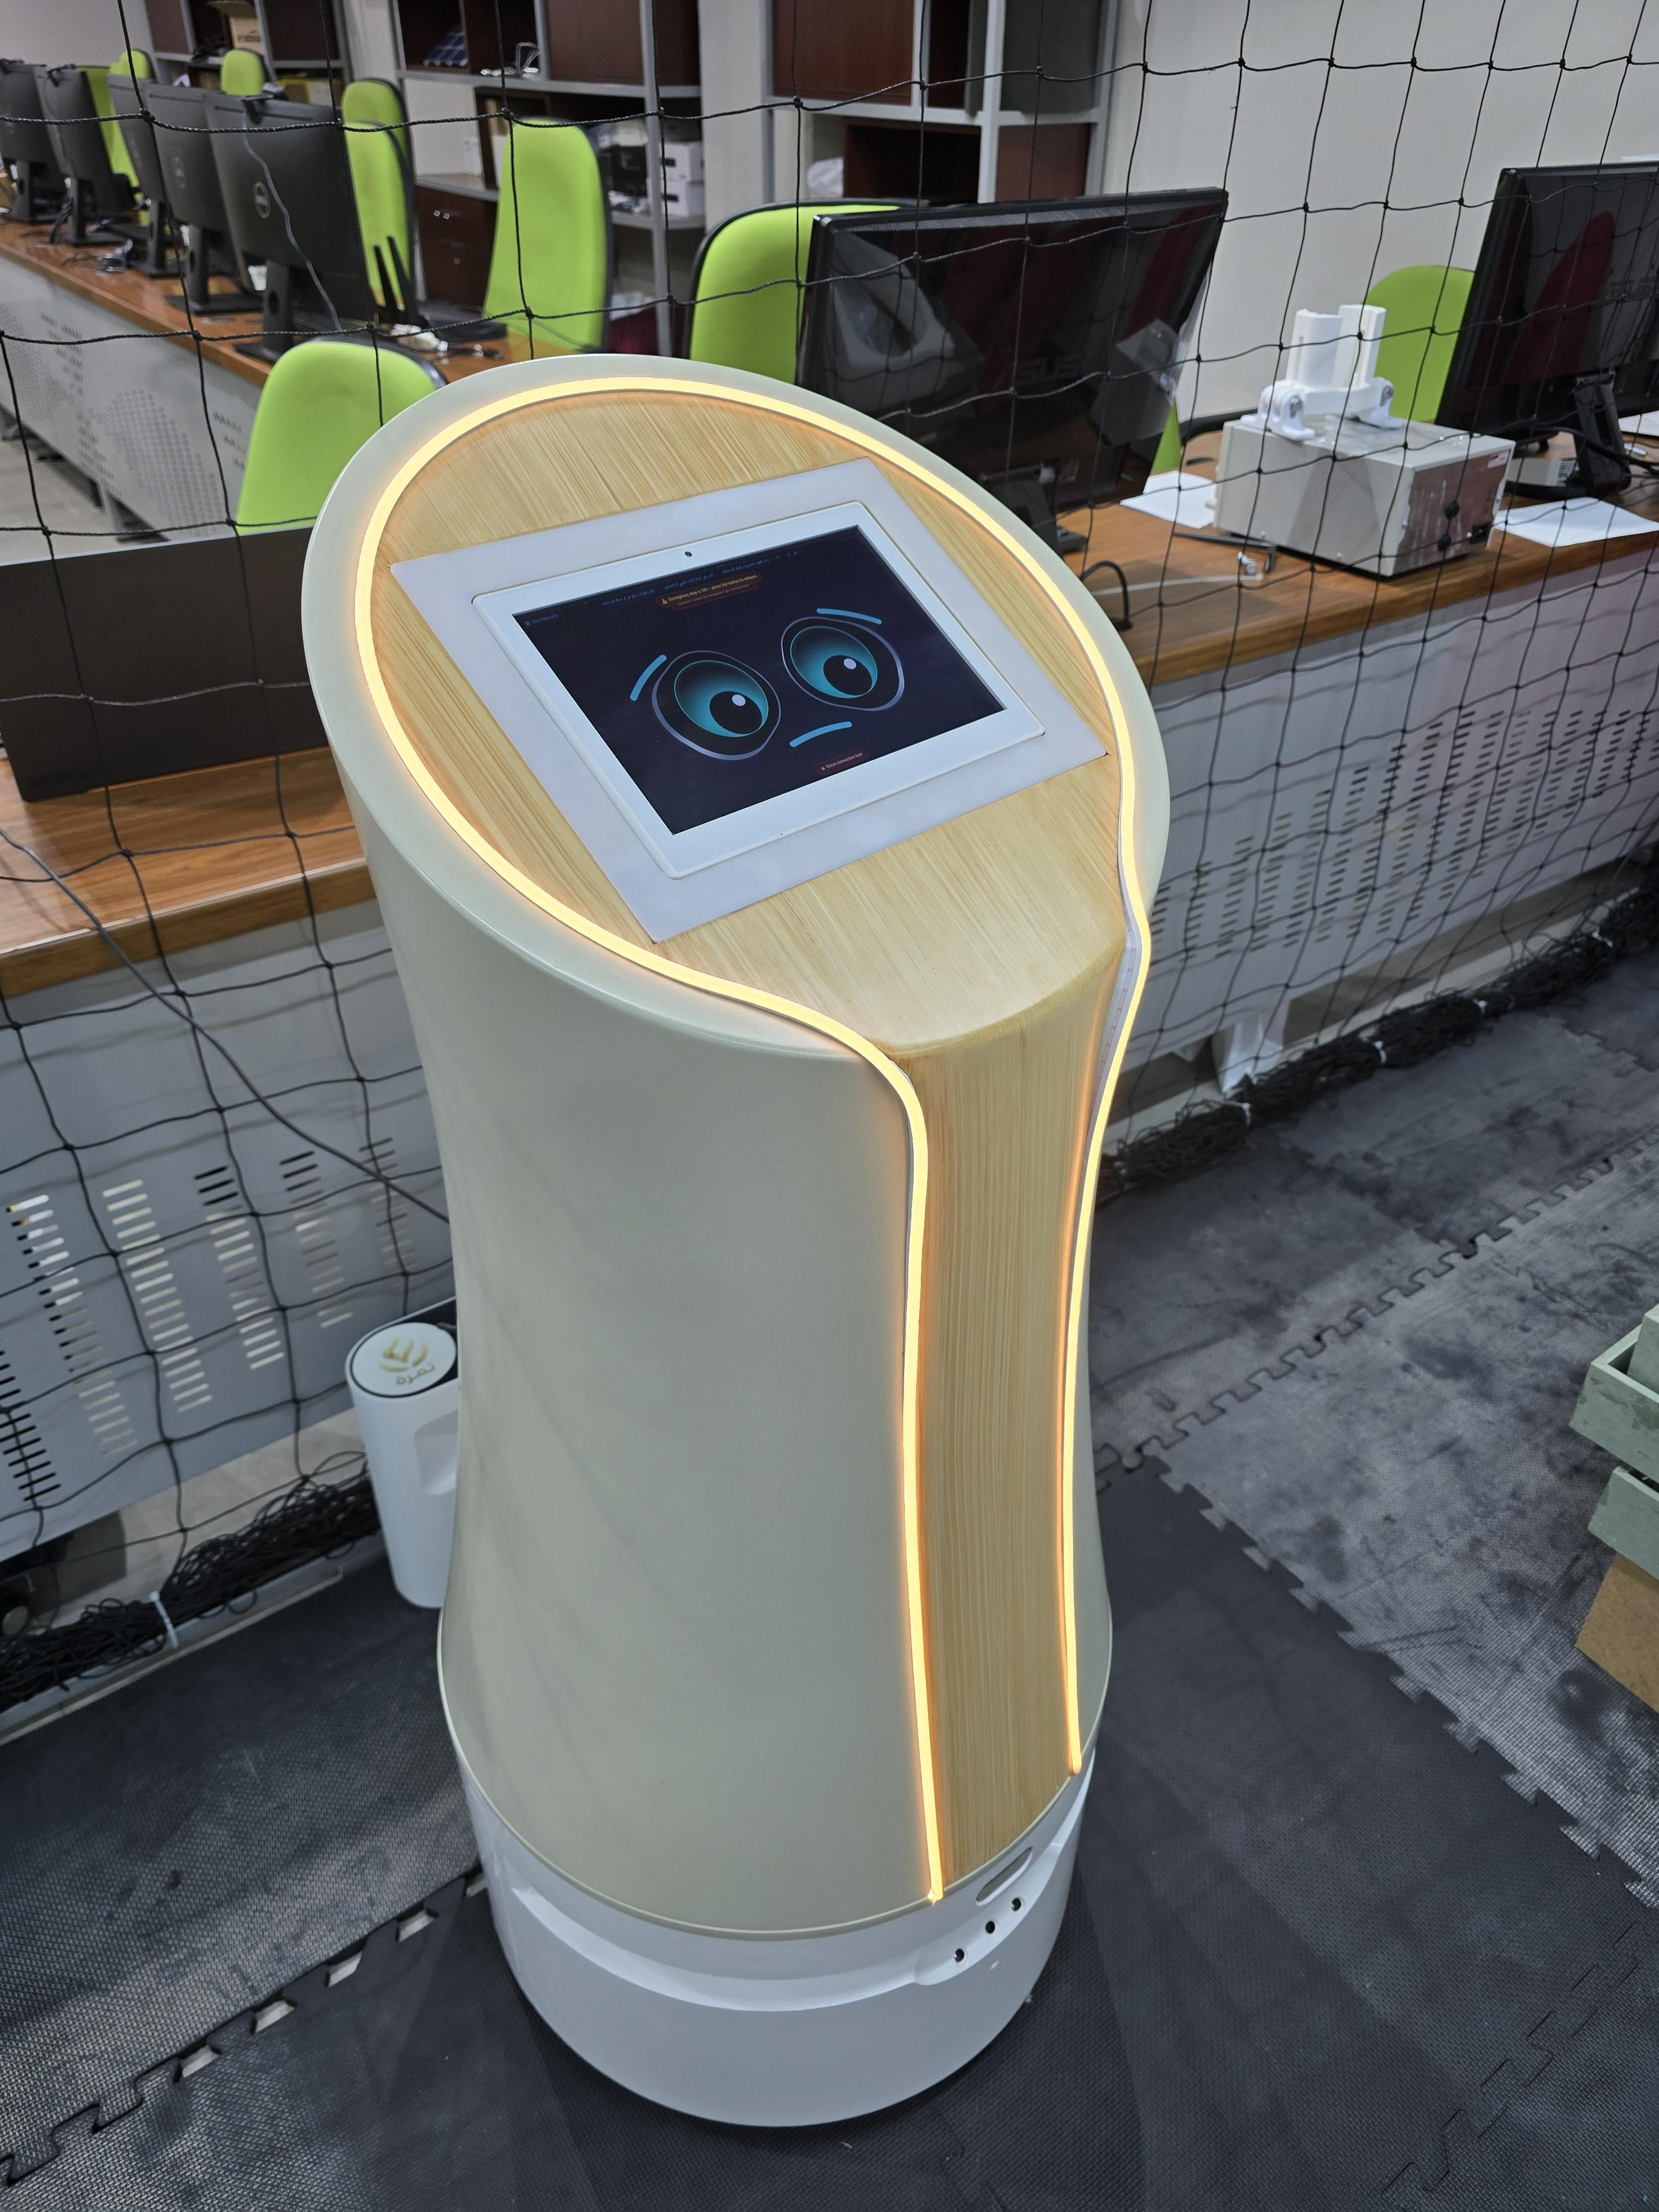
\includegraphics[width=\linewidth,height=6.5cm,keepaspectratio]{robot_top.jpg}
    \caption*{(c) Top view}
  \end{minipage}
  \caption{TAMRA after full integration. Front view (a) shows the oak-veneer panel, ambient LED strip, and the 10-inch display running the MACS animated face. Rear view (b) shows the open storage compartment, oak-veneer drawer, and the emergency-stop button. Top view (c) shows the display tilt and overall silhouette.}
  \label{fig:final_robot}
\end{figure}

\subsubsection{Display and Tablet Integration}

The human interface is a 10-inch industrial-grade Android tablet (off-shelf SoC, 2\,GB RAM, 1280$\times$800 IPS touch, Android~11) running in Fully Kiosk Browser kiosk mode. An industrial device was chosen for always-on operation and extended duty cycle.

\paragraph{Dual-network routing.}
The tablet must simultaneously maintain two network connections:
\begin{itemize}
  \item Ethernet to the robot chassis (\texttt{192.168.20.x} subnet) for low-latency ROS WebSocket communication
  \item WiFi to the campus network for cloud AI APIs and MQTT telemetry
\end{itemize}

Android's default behaviour routes all traffic over a single interface and drops the other. Eight solutions were evaluated -- Speedify dual-channel bonding, an ESP32 MQTT intermediary, Linux tablet swap, USB WiFi tethering, 4G/LTE dongle, disabling WiFi, USB wired tethering -- none were reliable or practical. The solution that worked was a boot daemon deployed via ADB (Android Debug Bridge) that sets static routes at startup: traffic to \texttt{192.168.20.x} is forced over \texttt{eth0}; all other traffic uses the \texttt{wlan0} default gateway. The daemon runs at boot and persists across Fully Kiosk Browser sessions.

% -------------------------------------
\subsection{Software Implementation}
% -------------------------------------

\subsubsection{Three-Tier Architecture}

The software is structured in three communicating tiers (Figure~\ref{fig:swarch}):

\begin{figure}[H]
  \centering
  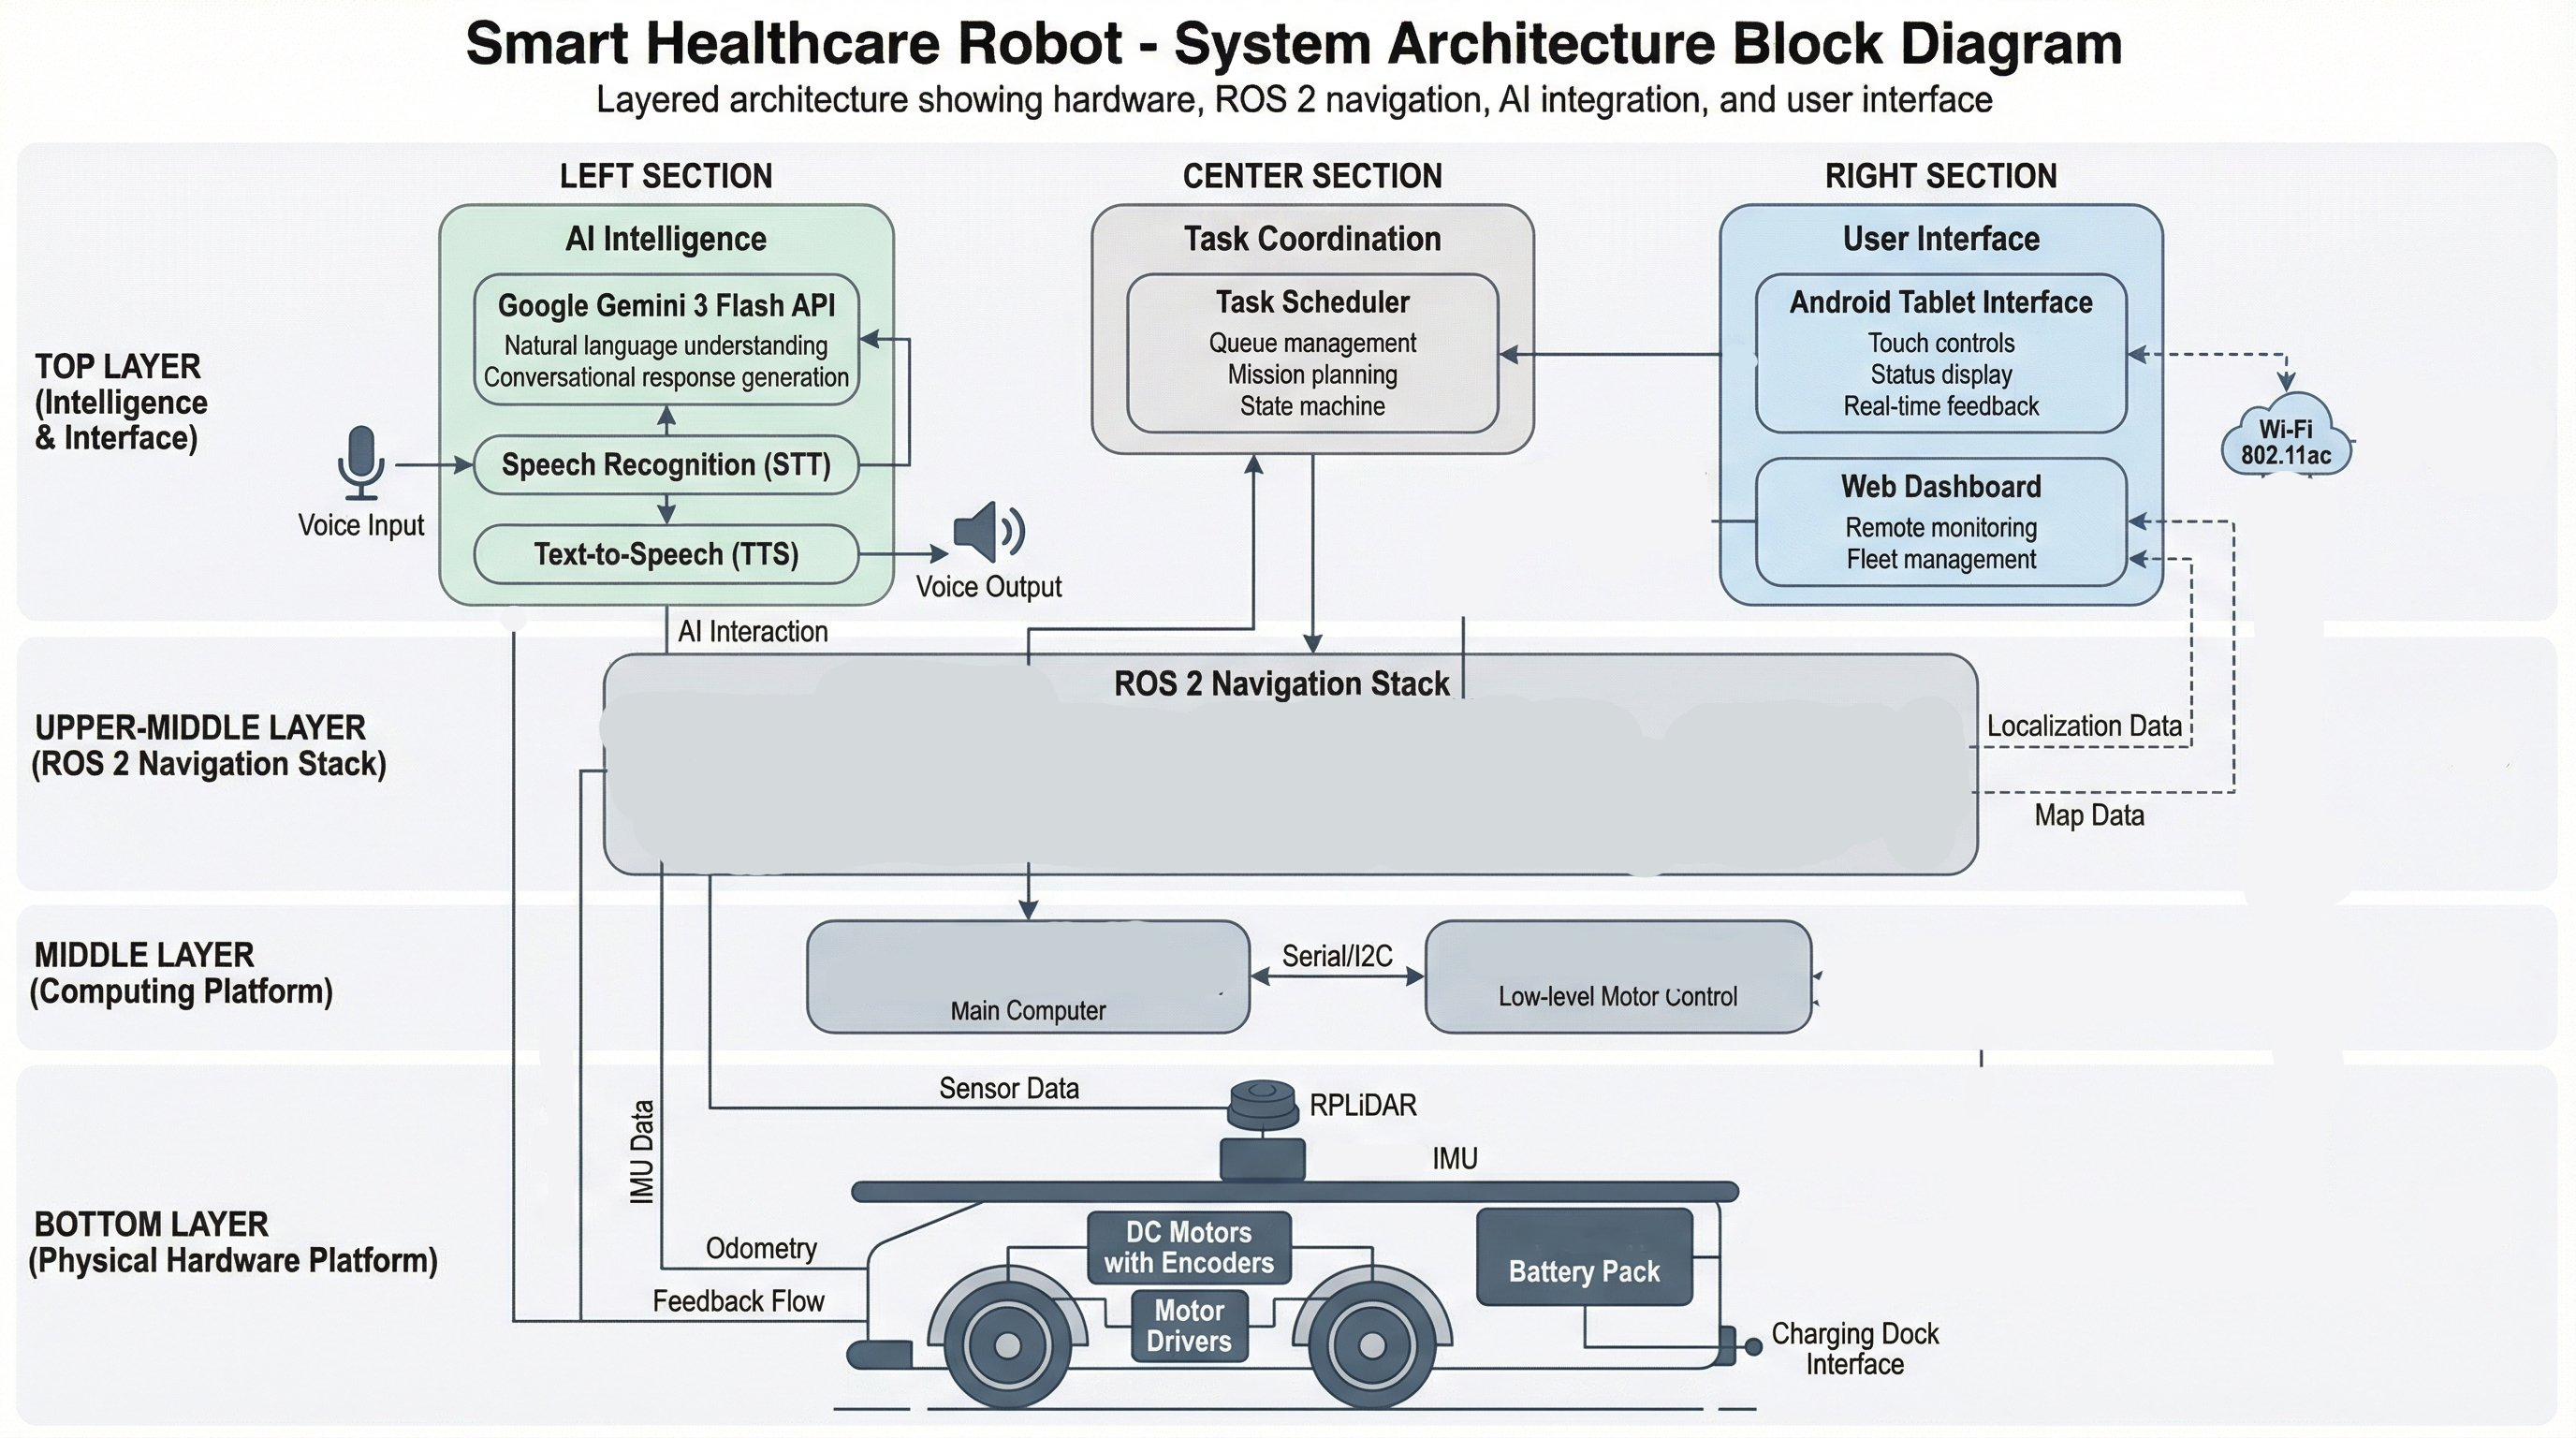
\includegraphics[width=0.92\textwidth]{system_block.png}
  \caption{Three-tier software architecture. The Robot Layer (iMRP500 SoC) runs ROS navigation and exposes sensor data over WebSocket. The Bridge Layer (tablet) hosts the mission engine, voice pipeline, and MQTT bridge. The Cloud Layer provides LLM orchestration, voice synthesis, and remote telemetry.}
  \label{fig:swarch}
\end{figure}

\begin{itemize}
  \item \textbf{Robot Layer}: The iMRP500 onboard SoC runs the ROS navigation stack, sensor drivers, and costmap pipeline. It exposes the rosbridge WebSocket on port~9090 and MJPEG video on port~9099.
  \item \textbf{Bridge Layer}: The tablet application -- a single self-contained HTML file -- connects to the robot over Ethernet WebSocket and to the cloud over WiFi. It hosts the mission engine, task queue, cron scheduler, MQTT bridge, and the MACS animated face. A single file requires no installation and can be updated by replacing it over ADB.
  \item \textbf{Cloud Layer}: Google Gemini~3 Flash provides LLM orchestration; ElevenLabs Conversational AI provides speech recognition and synthesis; HiveMQ Cloud provides TLS-encrypted MQTT brokering for remote telemetry and control.
\end{itemize}

\subsubsection{Semantic Task Orchestrator}

The orchestrator is the core software contribution of the project. It implements long-horizon task orchestration: a user speaks or types a natural language command in English or Arabic -- for example, ``take this to the pharmacy, then go check on room 5 and come back''--and the orchestrator converts it into a structured, executable sequence of robot actions that spans multiple locations, multiple steps, and multiple minutes of autonomous operation, with no further human input required.

The orchestrator invokes Gemini~3 Flash with a prompt that includes live robot context -- battery level, current position, known waypoints, and active task queue -- as dynamic variables. Gemini returns a typed mission plan:
\begin{equation}
  s_i \in \{\,\texttt{navigate}(w),\;\texttt{speak}(m),\;\texttt{display}(d),\;\texttt{photo},\;\texttt{wait}(t)\,\}
\end{equation}
where $w$ is a named waypoint, $m$ is a spoken message, $d$ is display content, and $t$ is a wait duration. The plan is returned as a server-sent event (SSE) stream, and the mission engine begins executing the first step before the full plan is generated. This streaming execution means the robot starts moving while the LLM is still producing later steps -- the primary mechanism for keeping voice-to-action latency below 3\,s.

\subsubsection{Voice Pipeline}

Three voice configurations were prototyped:
\begin{enumerate}
  \item \textbf{OpenAI Live Model}: Functional, but voice quality and tool-call latency felt unnatural in practice.
  \item \textbf{ElevenLabs standalone}: More natural voice synthesis, but overall round-trip latency was perceived as slow when combined with ROS command dispatch.
  \item \textbf{Gemini~3.1 Live (current)}: Gemini~3.1 Live provides real-time bidirectional audio processing with native tool-calling, eliminating the layered latency of the previous configurations. Tool calls (\texttt{robot\_control}, \texttt{plan\_and\_execute}, \texttt{cancel\_mission}) route directly to client-side handlers on the robot bridge.
\end{enumerate}

\subsubsection{Task Queue and Mission Engine}

The mission engine maintains a priority queue with five states:
\[
\textsc{pending} \;\to\; \textsc{running} \;\to\; \{\,\textsc{completed},\;\textsc{failed},\;\textsc{cancelled}\,\}
\]
A 1\,Hz tick dispatches navigation goals via the \texttt{/poi} ROS service. Four mission types are supported:
\begin{itemize}
  \item \textbf{GO\_TO}: Single-waypoint navigation
  \item \textbf{DELIVERY}: Multi-stop sequence (up to five waypoints) with confirmation at each stop
  \item \textbf{PATROL}: Looping route through a defined set of points of interest
  \item \textbf{AUTO\_CHARGE}: Battery-triggered return to dock (configurable threshold, default 20\%)
\end{itemize}
A built-in cron scheduler accepts standard five-field POSIX expressions for recurring autonomous missions.

\subsubsection{MQTT Bridge and Remote Dashboard}

Robot state is published at 1\,Hz over HiveMQ Cloud (WSS, TLS): pose, battery percentage, task queue, navigation status. Telemetry messages use MQTT QoS~1 (at-least-once delivery) to guarantee state updates reach the dashboard even under transient packet loss; control commands use QoS~2 (exactly-once) to prevent duplicate navigation goals. Large payloads (occupancy grid maps) are chunked into 64\,KB segments. The React-based remote dashboard renders a live occupancy grid map with robot pose overlay, task creation interfaces, task queue monitoring, cron schedule management, and a live MJPEG camera view for telepresence. Because it communicates exclusively over MQTT, it operates from any internet-connected device without VPN or special routing.

\subsubsection{Electrical Integration}

The added hardware (tablet, display, LED strip, kill switch) draws power from the iMRP500 chassis through a single regulated bus. The chassis exposes three external interfaces: a 24\,V power terminal, a hardware kill-switch terminal pair, and an Ethernet port. A 3\,A fuse protects the downstream rail; a DC--DC step-down converter regulates 24\,V to 12\,V for the tablet and the LED strip. The physical kill switch is wired in the normally-open (NO) configuration so that pressing it breaks the chassis safety loop and halts the drive motors per ISO~13850. Figure~\ref{fig:wiring} shows the wiring topology.

\begin{figure}[H]
\centering
\fcolorbox{black}{black}{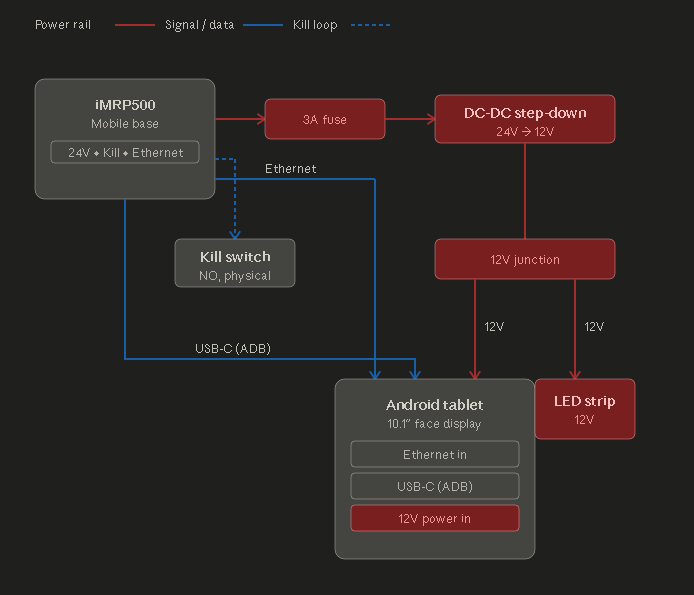
\includegraphics[width=0.65\linewidth]{wiring_diagram.png}}
\caption{TAMRA electrical integration. The iMRP500 chassis exposes three terminals: Ethernet, kill-switch pins, and 24\,V power. The kill switch is wired NO so activation opens the chassis safety loop per ISO~13850. The 24\,V rail passes through a 3\,A fuse and a DC--DC step-down converter to supply 12\,V to both the tablet and the LED strip. Three connections enter the tablet: 12\,V power, Ethernet from the chassis, and a persistent ADB USB link used by the dual-network boot daemon and for over-the-air HTML updates.}
\label{fig:wiring}
\end{figure}

% -------------------------------------
\subsection{System Integration and Testing}
% -------------------------------------

\subsubsection{Unit Tests}

Each subsystem was validated independently before integration:
\begin{itemize}
  \item \textbf{Navigation}: SLAM mapping completed; waypoint navigation confirmed $\pm$5\,cm accuracy; all four costmap layers verified against static and moving test obstacles.
  \item \textbf{Sensor pipeline}: All topics confirmed over WebSocket bridge. The self-diagnosis service (\texttt{/self\_diagnosis}) returned healthy status for LiDAR, network, encoders, battery, IR, ultrasonic, gyro, and depth camera.
  \item \textbf{Orchestrator}: Fifteen natural-language commands of increasing complexity (single waypoint, multi-stop delivery, conditional return) submitted in isolation. All fifteen produced valid, executable plans. First SSE step delivered within 1.2\,s on average.
  \item \textbf{Voice pipeline}: Tested for intelligibility, tool routing, and mid-speech interruption handling. All three tool calls routed correctly.
  \item \textbf{Body shell}: Footprint within 500\,mm confirmed; total height 900\,mm; added mass below 12\,kg; display tilt verified at 40$^{\circ}$; storage compartment functional; no sharp edges.
\end{itemize}

\subsubsection{Integration and Acceptance Testing}

The acceptance test validates all six customer requirements in a continuous sequence. A delivery mission was issued by voice: the robot navigated to a waypoint, announced its arrival verbally, waited for confirmation, then returned to the docking station and initiated autonomous charging. Remote control was exercised simultaneously from the MQTT dashboard on a separate device. A voice interruption test confirmed that an in-flight patrol mission could be cancelled and replaced with a new navigation goal within 2\,s of the voice command.

All engineering requirements defined in Chapter~3 were met. The team adhered to all applicable project constraints throughout implementation, including the 300\,OMR body shell budget, the 500\,mm chassis footprint, the 12\,kg added-mass limit, and the ISO~13482 and ISO~13850 safety standards.

% -------------------------------------
\subsection{Results}
\label{sec:results}
% -------------------------------------

\subsubsection{Voice-to-Action Latency}

End-to-end latency from voice command completion to first robot motion was measured across 20 trials ($N=20$). Figure~\ref{fig:latency_bar} shows the per-component breakdown.

\begin{figure}[H]
\centering
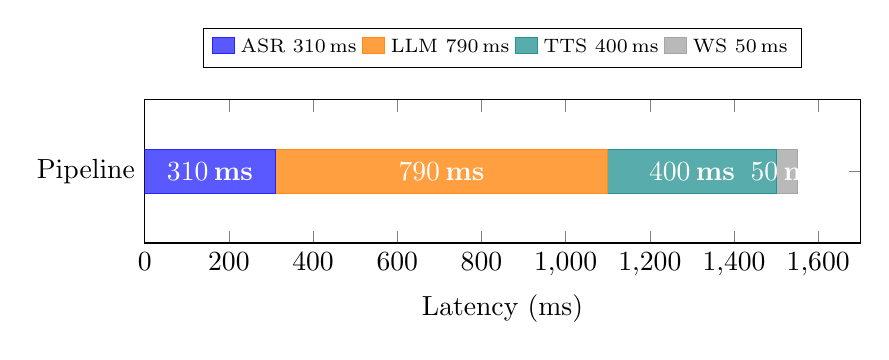
\begin{tikzpicture}
\begin{axis}[
    xbar stacked,
    width=0.88\linewidth,
    height=3.4cm,
    xlabel={Latency (ms)},
    ytick={1},
    yticklabels={Pipeline},
    xmin=0, xmax=1700,
    ymin=0.3, ymax=1.7,
    bar width=16pt,
    legend style={at={(0.5,1.22)},anchor=south,legend columns=4,font=\scriptsize},
    enlarge y limits=0.5,
    nodes near coords={\pgfmathprintnumber\pgfplotspointmeta\,ms},
    every node near coord/.append style={font=\tiny,text=white,font=\bfseries},
]
\addplot[fill=blue!65,draw=blue!85]     coordinates {(310,1)};
\addplot[fill=orange!75,draw=orange!90] coordinates {(790,1)};
\addplot[fill=teal!65,draw=teal!85]     coordinates {(400,1)};
\addplot[fill=gray!55,draw=gray!70]     coordinates {( 50,1)};
\legend{ASR 310\,ms, LLM 790\,ms, TTS 400\,ms, WS 50\,ms}
\end{axis}
\end{tikzpicture}
\caption{Voice-to-action latency breakdown ($N=20$, mean total 1{,}550\,ms, $\sigma=310$\,ms). LLM tool-call resolution dominates at 51\%. All 20 trials completed below the 3\,s engineering requirement (max observed: 2.41\,s). Streaming SSE execution further reduces perceived latency by dispatching the first navigation command before the complete plan is generated.}
\label{fig:latency_bar}
\end{figure}

\subsubsection{MQTT Telemetry Latency}

Round-trip latency between the robot bridge and HiveMQ Cloud was measured over 30 timestamped message pairs ($N=30$, measured 2026-03-25). Figure~\ref{fig:mqtt_hist} shows the distribution.

\begin{figure}[H]
\centering
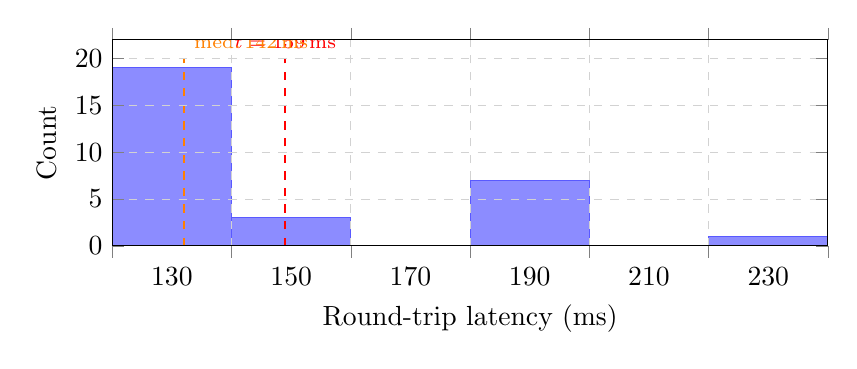
\begin{tikzpicture}
\begin{axis}[
    ybar interval,
    width=0.88\linewidth,
    height=4.2cm,
    xlabel={Round-trip latency (ms)},
    ylabel={Count},
    xmin=130, xmax=250,
    ymin=0, ymax=22,
    xtick={130,150,170,190,210,230,250},
    ymajorgrids=true,
    grid style={dashed,gray!35},
    area style,
]
\addplot[fill=blue!45,draw=blue!65] coordinates {
    (130,19)(150,3)(170,0)(190,7)(210,0)(230,1)(250,0)
};
\draw[dashed,red,thick] (axis cs:159,0)--(axis cs:159,20)
    node[above,font=\scriptsize,red]{$\bar{t}=159$\,ms};
\draw[dashed,orange,thick] (axis cs:142,0)--(axis cs:142,20)
    node[above right,font=\scriptsize,orange]{med.\,142\,ms};
\end{axis}
\end{tikzpicture}
\caption{MQTT round-trip latency distribution ($N=30$). Mean 159\,ms, median 142\,ms, 95th percentile 207\,ms, max 243\,ms. All 30 messages delivered below 250\,ms. The bimodal distribution reflects occasional DPI buffering on the campus WiFi (eduroam); direct robot control uses the local Ethernet path and is unaffected. Telepresence video latency (MJPEG stream from robot to dashboard) was separately measured at 130\,ms under the same network conditions.}
\label{fig:mqtt_hist}
\end{figure}

\subsubsection{Navigation and Orchestrator}

Waypoint navigation accuracy of $\pm$5\,cm was confirmed through repeated trials across three defined waypoints. The 4-layer costmap successfully avoided all static and dynamic test obstacles. All fifteen orchestrator test commands produced valid, executable mission plans with no hallucinated waypoints or malformed step types.

% -------------------------------------
\subsection{Budget Summary}
% -------------------------------------

\begin{table}[H]
\centering
\small
\caption{Hardware procurement costs.}
\label{tab:budget}
\setlength{\tabcolsep}{6pt}
\begin{tabular}{@{} >{\raggedright\arraybackslash}p{6.0cm} r @{}}
\toprule
\textbf{Item} & \textbf{OMR} \\
\midrule
iMRP500 chassis (incl.\ shipping)         & 850 \\
10-inch 1080p industrial touch display    & 77 \\
Body shell (MDF, veneer, acrylic, paint)  & 300 \\
Cables, fasteners, connectors            & 73 \\
\midrule
\textbf{Total}                           & \textbf{1{,}300} \\
\bottomrule
\end{tabular}
\end{table}

\noindent At approximately USD~3{,}200, TAMRA delivers autonomous navigation, conversational AI, item delivery, and remote telepresence -- a 73\% cost reduction against the nearest commercial platform with comparable capability \cite{pudubot2,m2medical}.

% -------------------------------------
\subsection{Standards Compliance}
% -------------------------------------

\begin{itemize}
  \item \textbf{ISO~13482:2014}: Navigation speed (0.8\,m/s) and inflation radius (0.8\,m) satisfy the velocity and proximity limits for robots in human-shared spaces.
  \item \textbf{ISO~13850}: Hardware E-stop relay tested; robot halts within one control cycle on activation. Soft-stop service provides a software-level equivalent.
  \item \textbf{ITU-T H.264}: Camera streams use standard compressed formats compatible with web browsers.
  \item \textbf{IEEE~802.11}: MQTT and cloud AI APIs operate over standard campus WiFi with no infrastructure modifications.
\end{itemize}

% -------------------------------------
\subsection{Conclusion}
% -------------------------------------

Chapter~5 documented the full implementation of TAMRA. The iMRP500 was selected after a six-platform comparison and reverse-engineered to expose its full sensor suite over a documented WebSocket API. The body shell was designed through a three-stage workflow -- concept rendering, AI-assisted 3D mesh synthesis, and parametric Fusion~360 refinement -- and fabricated locally in Muscat within budget and mass constraints. The three-tier software stack was developed in parallel with hardware procurement. Measured results confirm voice-to-action latency of $1{,}550 \pm 310$\,ms (all 20 trials below 3\,s), MQTT round-trip of $159 \pm 30$\,ms, navigation accuracy of $\pm$5\,cm, and 100\% plan-generation success across 15 orchestrator test commands.


% Chapter 6: Conclusions and Future Works
\chapterintro{6}{Conclusions and Future Works}{This chapter summarises the engineering contributions of the project, identifies areas for improvement, and outlines future development directions toward full-scale service robot deployment.}
\section{Conclusions and Future Works}
\label{sec:conclusion}
% ============================================================
%  Chapter 6 -- Conclusions and Future Works
% ============================================================

\subsection{Project Summary}

This project produced TAMRA (Task-Agnostic Modular Robotic Apparatus), an autonomous mobile robot that integrates LiDAR-based navigation, LLM-driven semantic task orchestration, real-time voice interaction, item delivery, and remote telepresence on a single platform at a total hardware cost of USD~3{,}240.

The work spanned two semesters. The first semester built a thorough foundation through literature review, requirements formalisation, and AHP-based architecture selection, centred on TurtleBot~4 and iCreate~3. The second semester realised the system in hardware and software, navigating two significant decisions: a platform transition forced by the iRobot bankruptcy and the structural limitations of educational bases, and a scope refinement from a strictly medical device to a general-purpose autonomous service robot -- validated in a healthcare corridor but designed to generalise across any service environment. This reframing was the difference between a system that could be deployed within the project timeline and one that could not.

\paragraph{Technical contributions.}
The three engineering contributions are:
\begin{enumerate}
  \item \textbf{Hybrid hardware platform}: An industrial chassis (iMRP500) combined with a custom-fabricated ergonomic body shell, designed in Oman within a 300\,OMR budget. The design workflow -- generative rendering to 3D mesh synthesis to parametric Fusion~360 refinement -- is a reproducible methodology for human-facing robot aesthetics.
  \item \textbf{Semantic task orchestrator}: A streaming LLM pipeline (Gemini~3 Flash) that converts free-form English or Arabic voice commands into typed, multi-step mission plans executed in real time by an on-device mission engine, with voice-to-action latency of $1{,}550 \pm 310$\,ms ($N=20$, all trials below 3\,s).
  \item \textbf{Layered software architecture}: A three-tier stack (ROS~2 navigation, tablet bridge application, cloud AI and MQTT telemetry) that separates concerns cleanly and enables the full system to be updated by replacing a single HTML file over ADB.
\end{enumerate}

% -------------------------------------
\subsection{Areas of Improvement}
% -------------------------------------

\begin{itemize}
  \item \textbf{Navigation in high-traffic corridors}: The global planner replans inefficiently when many moving obstacles appear simultaneously, causing brief stops. A more adaptive local planner or an upgraded dynamic obstacle layer would improve fluency \cite{chen2022}.
  \item \textbf{Voice recognition in ambient noise}: ASR accuracy degrades in noisy reception-area environments. A directional microphone array or server-side noise suppression tuned to indoor acoustic profiles would address this.
  \item \textbf{Display brightness}: The 10-inch panel has limited visibility near windows in strong ambient light. A higher-brightness panel or an anti-glare acrylic coating would improve legibility.
  \item \textbf{Autonomous docking reliability}: Localisation drift accumulated over a long shift can cause the robot to miss the dock contact. A short-range UWB or IR beacon at the dock for fine-approach correction would bring docking success rate to the 95\% engineering target under all conditions.
  \item \textbf{Arabic language coverage}: The orchestrator and voice pipeline support Arabic, but systematic accuracy evaluation with native speakers has not been conducted. This should be completed before Arabic is offered as a primary interaction language.
\end{itemize}

% -------------------------------------
\subsection{Future Works}
% -------------------------------------

\paragraph{Hardware call buttons (433\,MHz local RF).}
Physical call buttons distributed around a building would allow any user to summon the robot without a phone or voice interaction. The buttons communicate over 433\,MHz RF -- a licence-free band that operates entirely without external infrastructure (no router, no WiFi, no internet). The robot carries a 433\,MHz receiver module. This makes the system operable in areas with poor WiFi coverage and removes the dependency on smartphone literacy for the most basic use case.

\paragraph{WhatsApp integration.}
WhatsApp is ubiquitous in Oman and the wider GCC region. Integrating TAMRA with the WhatsApp Business Cloud API would allow users to send a message to summon the robot, request a delivery, or check its status using an application they already have on their phone. The interaction is intuitive, requires no new app installation, and creates a persistent conversation log. The MQTT bridge already handles the back-end; adding a WhatsApp webhook is an incremental step.

\paragraph{Multi-robot fleet coordination.}
The MQTT bridge architecture supports multiple robots publishing to distinct topic namespaces from a single dashboard. The next step is a fleet manager that distributes tasks across a pool of TAMRA units, prevents waypoint conflicts, and rebalances loads when one robot goes to charge. ROS~2's DDS-based distributed layer provides the underlying communication primitives.

\paragraph{Hospital Information System integration.}
Connecting TAMRA to a hospital HIS or EHR via HL7/FHIR interfaces would allow the orchestrator to read room assignments, scheduled deliveries, and ward status dynamically rather than relying on manually configured waypoints. This is the primary technical path toward full clinical deployment \cite{jmir2024}.

\paragraph{End-user experience refinement.}
The current interface is functional but not yet polished. Planned refinements include animated contextual responses on the display (the MACS face reacts to task state), proactive status updates to the requesting user over WhatsApp, smoother handoff between voice interaction and autonomous navigation modes, and configurable personality profiles suited to different environments (clinical, hospitality, campus).

\paragraph{UV-C disinfection module.}
The upper tray mounting points provide a structural basis for a UV-C emitter for autonomous disinfection runs during off-peak hours, with safety interlocks disabling the emitter whenever occupancy is detected \cite{sciencedirect2021}.

\paragraph{Longitudinal field study.}
Laboratory bench tests cannot substitute for real deployment. A structured field study in a hospital, hotel, or campus building -- measuring navigation reliability, staff workflow impact, and maintenance burden over multiple weeks -- would provide the empirical grounding the system needs before broader rollout.


% ============================================================
% REFERENCES
% ============================================================
\newpage
\bibliographystyle{unsrt}
\bibliography{references/references}

% ============================================================
% APPENDICES
% ============================================================
\newpage
\appendix
\section{Appendix: Standards and Regulatory References}
\label{sec:appendix}

\subsection{ISO Standards}
This project references the following international safety and technical standards:

\begin{itemize}[leftmargin=*]
    \item \textbf{ISO 13482:2014} -- Robots and robotic devices -- Safety requirements for personal care robots \\
    \url{https://www.iso.org/standard/53820.html}
    
    
    \item \textbf{ISO 13850:2015} -- Safety of machinery -- Emergency stop function -- Principles for design \\
    \url{https://www.iso.org/standard/59970.html}
\end{itemize}

\subsection{Data Protection and Privacy Regulations}
\begin{itemize}[leftmargin=*]
    \item \textbf{GDPR (General Data Protection Regulation)} -- Regulation (EU) 2016/679 of the European Parliament and of the Council on the protection of natural persons with regard to the processing of personal data \\
    \url{https://eur-lex.europa.eu/eli/reg/2016/679/oj}
    
    \item \textbf{HIPAA (Health Insurance Portability and Accountability Act)} -- U.S. Department of Health \& Human Services regulations for protecting sensitive patient health information \\
    \url{https://www.hhs.gov/hipaa/index.html}
\end{itemize}

\end{document}
